\documentclass{article}


%pacchetti extra da scaricare dblfloatfix, fancyhdr
\usepackage{fancyhdr}%creazione header-footer
\usepackage{graphicx} %serve per inserire immagini
%\usepackage{dblfloatfix} %serve per posizionare gli elementi dove si vuole
\usepackage[hidelinks]{hyperref} %serve per i link
\usepackage{tikz}
% \usepackage{tgadventor} % font
\usepackage[useregional=numeric,showseconds=true,showzone=false]{datetime2}
\usepackage{caption}
\usepackage{geometry}
\usepackage{setspace}
\usepackage{eurosym}
\usepackage[italian]{babel}
\usepackage[hidelinks]{hyperref}
\usepackage{tabularx}
\usepackage{longtable}
\usepackage{float}

\usepackage{graphicx}
% Margini della pagina
\geometry{a4paper, margin=1in}

% Intestazione personalizzata
\pagestyle{fancy}
\fancyhf{}
\fancyhead[L]{Code7Crusaders - Software Development Team}
\fancyhead[R]{\thepage}

% Spaziatura delle righe
\setstretch{1.2}

\begin{document}

\begin{titlepage} 

    \AddToHookNext{shipout/background}{
    \begin{tikzpicture}[remember picture,overlay]
    \node at (current page.center) {
    
\includegraphics{../../../img/background.png}
    };
    \end{tikzpicture}
    }

    \centering
    \vspace*{2cm}
    
    
\includegraphics[width=0.3\textwidth]{../../../img/logo/7Crusaders_logo.png} % Aggiungi il logo qui
    \vspace{1cm}
    
    {\Huge \textbf{Code7Crusaders}}\\
    \vspace{0.5cm}
    {\Large Software Development Team}\\
    \vspace{2cm}
    
    \large \textbf{Manuale Utente}
    \vspace{3.9cm}

    \textbf{Membri del Team:}\\
    Enrico Cotti Cottini, Gabriele Di Pietro, Tommaso Diviesti \\
    Francesco Lapenna, Matthew Pan, Eddy Pinarello, Filippo Rizzolo \\
    \vspace{0.5cm}
    
    \vspace{1cm}
\end{titlepage}



\newpage
%------------------------Versioni
\begin{table}[h]
    \centering
    \renewcommand{\arraystretch}{1.2}
    \setlength{\tabcolsep}{5pt}
    \begin{tabular}{|c|c|c|c|m{0.35\textwidth}|}
        \hline
        \textbf{Ver} & \textbf{Data} & \textbf{Redattore} & \textbf{Verificatore} & \textbf{Descrizione} \\
        \hline
        0.2 & 29/03/2025 & Filippo Rizzolo & & Stesura \\
        0.1 & 1/03/2025 & Eddy Pinarello & Filippo Rizzolo & Prima stesura del documento \\
        \hline
    \end{tabular}
\end{table}

%----------------

\newpage
\tableofcontents
\listoftables
\listoffigures

\newpage

\section{Introduzione}

\subsection{Scopo del documento}
Questo documento ha lo scopo di definire le regole e le procedure che ogni membro del team deve seguire durante 
lo sviluppo del progetto. In particolare, mira a stabilire il \textit{Way of Working} del gruppo. 

La sua redazione inizia nelle prime fasi del progetto e continua anche durante le fasi successive, 
per essere costantemente aggiornato e adattato alle esigenze del team. 

Il processo seguirà le linee guida dello standard ISO/IEC 12207:1995, suddivise in:
\begin{itemize}
    \item Processi primari
    \item Processi di supporto
    \item Processi organizzativi
\end{itemize}


\subsection{Scopo del progetto}
Il progetto si propone di sviluppare un Assistente Virtuale intelligente per aziende che operano nel 
settore della vendita multiprodotto. Questo assistente avrà il compito di semplificare l'accesso alle 
informazioni sui prodotti disponibili, rispondendo alle domande più frequenti poste dai clienti in modo rapido ed efficace.

Grazie all'uso di tecnologie avanzate come il \href{https://code7crusaders.github.io/docs/RTB/documentazione_interna/glossario.html#machine-learning}{Machine Learning\textsuperscript{G}} e il \href{https://code7crusaders.github.io/docs/RTB/documentazione_interna/glossario.html#natural-language-processing-nlp}{Natural Language Processing\textsuperscript{G}}, 
il sistema sarà in grado di analizzare i dati contenuti nei cataloghi aziendali e negli archivi digitali, 
fornendo risposte precise e personalizzate.

L’obiettivo principale è ridurre la dipendenza dagli specialisti aziendali, che attualmente rappresentano 
l’unico canale di accesso per ottenere dettagli approfonditi sui prodotti. Questo migliorerà l’efficienza 
operativa, ottimizzerà le risorse e offrirà una migliore esperienza ai clienti, che potranno interagire con 
il sistema in modo intuitivo e diretto attraverso piattaforme digitali come siti web o chatbot.

In sintesi, il progetto intende rendere l'accesso alle informazioni aziendali più semplice, veloce e scalabile, 
migliorando al contempo la qualità del servizio offerto ai clienti.


\subsection{Glossario}
Per evitare ambiguità e facilitare la comprensione del documento, si farà uso di un glossario, 
contenente la definizione dei termini tecnici e degli acronimi utilizzati, 
che sarà incluso all'interno del file \textit{glossario}.


\subsection{Riferimenti}
\subsubsection{Normativi}
\begin{itemize}
	\item \textbf{Capitolato C7:} \\ \url{https://www.math.unipd.it/~tullio/IS-1/2024/Progetto/C7.pdf}
	\item \textbf{ISO/IEC 12207:1995} \\ \url{https://www.math.unipd.it/~tullio/IS-1/2009/Approfondimenti/ISO_12207-1995.pdf}
\end{itemize}

\subsubsection{Informativi}
\begin{itemize}
    \item\textbf{Glossario RTB}\\ \url{https://code7crusaders.github.io/docs/RTB/documentazione_interna/glossario.html}
    \item\textbf{Documentazione Git}\\ \url{https://git-scm.com/docs}
    \item\textbf{Documentazione Latex}\\ \url{https://www.latex-project.org/help/documentation/}

\end{itemize}


\newpage

\section{Requisiti}
In questa sezione vengono presentati i requisiti emersi durante l'attività di analisi, 
condotta a partire dai casi d'uso, dall'esame del capitolato d'appalto e dagli incontri, 
sia interni che con il proponente. 

\subsection{Classificazione dei requisiti}
I requisiti sono classificati in tre categorie principali:  
\begin{itemize}
    \item \textbf{Funzionali}: riguardano l'usabilità del prodotto finale;  
    \item \textbf{Di qualità}: includono gli strumenti e la documentazione da fornire;  
    \item \textbf{Di vincolo}: fanno riferimento alle tecnologie da utilizzare.
\end{itemize}
Per ciascun requisito è indicato:
\begin{itemize}
    \item \textbf{Codice Identificativo}: codice univoco che identifica il requisito;
    \item \textbf{Descrizione}: breve spiegazione del requisito;
    \item \textbf{Fonte}: origine del requisito (es. capitolato, interno, ecc..);
    \item \textbf{Priorità}: importanza del requisito rispetto agli altri;
\end{itemize} 

\subsection{Fonti dei requisiti}
I requisiti sono stati identificati a partire dalle seguenti fonti:
\begin{itemize}
    \item \textbf{Capitolato}: Requisiti individuati tramite analisi del capitolato;
    \item \textbf{interno}: requisiti individuati durante riunioni interne al gruppo di lavoro;
    \item \textbf{Esterno}: requisiti individuati durante incontri con il proponente;
    \item \textbf{Piano di Qualifica}: Requisiti necessari per rispettare standard di qualità definiti nel documento Piano di Qualifica;
    \item \textbf{Norme di Progetto}: Requisiti necessari per rispettare le norme di progetto definite nel documento Norme di Progetto;
\end{itemize}

\subsection{Codifica dei requisiti}
I requisiti sono codificati come segue: \textbf{R[Tipo][Importanza][Numero]}
\newline
Dove \textbf{Tipo} può essere:
\begin{itemize}
    \item \textbf{F (funzionale)}
    \item \textbf{Q (di qualità)}
    \item \textbf{V (di vincolo)}
\end{itemize}
\textbf{Importanza} può essere:
\begin{itemize}
    \item \textbf{O (obbligatorio)}
    \item \textbf{D (desiderabile)}
    \item \textbf{F (facoltativo )}
\end{itemize}
\textbf{Numero} è un numero identificativo univoco del requisito.

\textbf{Esempio}:
\begin{itemize}
    \item RFO1: Requisito funzionale obbligatorio numero 1
    \item RQD2: Requisito di qualità desiderabile numero 2
    \item RVF3: Requisito di vincolo facoltativo numero 3
\end{itemize}

\pagebreak
\subsection{Requisiti funzionali}
\begin{longtable}{|>{\centering\arraybackslash}m{0.10\textwidth}|>{\centering\arraybackslash}m{0.20\textwidth}|>{\centering\arraybackslash}m{0.6\textwidth}|}
	\hline
	\textbf{Codice} & \textbf{Fonte} & \textbf{Descrizione}\\\hline
	\endfirsthead
	\hline
	\textbf{Codice} & \textbf{Fonte} & \textbf{Descrizione}\\\hline
	\endhead
	\hline
	RFO1            & Capitolato    & Requisito funzionale obbligatorio numero 1
	\\\hline
	\caption{Requisiti funzionali}
\end{longtable}

\pagebreak
\subsubsection{Requisiti Qualitativi}
\begin{longtable}{|>{\centering\arraybackslash}m{0.10\textwidth}|>{\centering\arraybackslash}m{0.20\textwidth}|>{\centering\arraybackslash}m{0.6\textwidth}|}
	\hline
	\textbf{Codice} & \textbf{Fonte} & \textbf{Descrizione}\\\hline
	\endfirsthead
	\hline
	\textbf{Codice} & \textbf{Fonte} & \textbf{Descrizione}\\\hline
	\endhead
	\hline
	RQD2            & Interno    & Requisito di qualità desiderabile numero 2
	\\\hline
	\caption{Requisiti Qualitativi}
\end{longtable}

\pagebreak
\subsubsection{Requisiti di vincolo}
\begin{longtable}{|>{\centering\arraybackslash}m{0.10\textwidth}|>{\centering\arraybackslash}m{0.20\textwidth}|>{\centering\arraybackslash}m{0.6\textwidth}|}
	\hline
	\textbf{Codice} & \textbf{Fonte} & \textbf{Descrizione}\\\hline
	\endfirsthead
	\hline
	\textbf{Codice} & \textbf{Fonte} & \textbf{Descrizione}\\\hline
	\endhead
	\hline
	RVF3            & Esterno    & Requisito di vincolo facoltativo numero 3
	\\\hline
	\caption{Requisiti di vincolo}
\end{longtable}

\subsubsection{Requisiti sistema operativo}

\subsubsection{Requisiti di prestazione}

\subsubsection{Requisiti di sicurezza}

\pagebreak
\subsection{Tracciamento}
\subsubsection{Requisito - Fonte}
\begin{longtable}{|>{\centering\arraybackslash}m{0.40\textwidth}|>{\centering\arraybackslash}m{0.4\textwidth}|}
	\hline
	\textbf{Requisito} & \textbf{Fonte} 
	\endfirsthead
	\hline
	\textbf{Requisito} & \textbf{Fonte} 
	\endhead
	\hline
	RFO1            & Capitolato    
	\\\hline
    RQD2            & Interno
    \\\hline
    RVF3            & Esterno
    \\\hline
	\caption{Requisito - Fonte}
\end{longtable}




\newpage

% \section{Istruzioni all'uso}
% \subsection{Pagine User}
% In questa Sezione mostriamo le pagine riservate all'utente.
% \subsubsection{Landing page}
% All'avvio del prodotto verrà visualizzata la landing page, che presenta il logo dell'assistente virtuale e un messaggio di benvenuto. In questa fase, l'utente può scegliere di accedere al sistema.
% \begin{figure}[h!]
%     \centering
%     \includegraphics[width=0.8\textwidth]{./img/landingPage.png}
%     \caption{Schermata della landing page}
% \end{figure}

% \subsubsection{Pagina di Accesso}
% Cliccando sul bottone blu si passerà direttamente alla pagina di accesso, dove l'utente dovrà inserire le proprie credenziali (\textit{username} e \textit{password}) per autenticarsi.
% \begin{figure}[h!]
%     \centering
%     \includegraphics[width=0.8\textwidth]{./img/paginaAccesso.png}
%     \caption{Schermata della pagina di accesso}
% \end{figure}

% \subsubsection{Pagina di Registrazione}
% Nel caso in cui non si possieda un account, è possibile registrarsi dalla pagina di registrazione cliccando sul link presente nella pagina di autenticazione.
% Qui l'utente dovrà inserire i campi obbligatori \{ \textit{username; password; email; nome; cognome} \} e volendo opzionalmente può inserire il numero di telefono.
% \begin{figure}[h!]
%     \centering
%     \includegraphics[width=0.8\textwidth]{./img/paginaRegistrazione.png}
%     \caption{Schermata della pagina di registrazione}
% \end{figure}

% \subsubsection{Schermata iniziale}
% Una volta effettuato l'accesso verremo accolti da questa Schermata iniziale composta da 3 elementi, una navbar superiore, una navbar laterale e il contenuto della pagina. Da qui è possibile iniziare una conversazione mettendo il titolo della conversazione e schiacciando il bottone: "inizia la conversazione".
% \begin{figure}[h!]
%     \centering
%     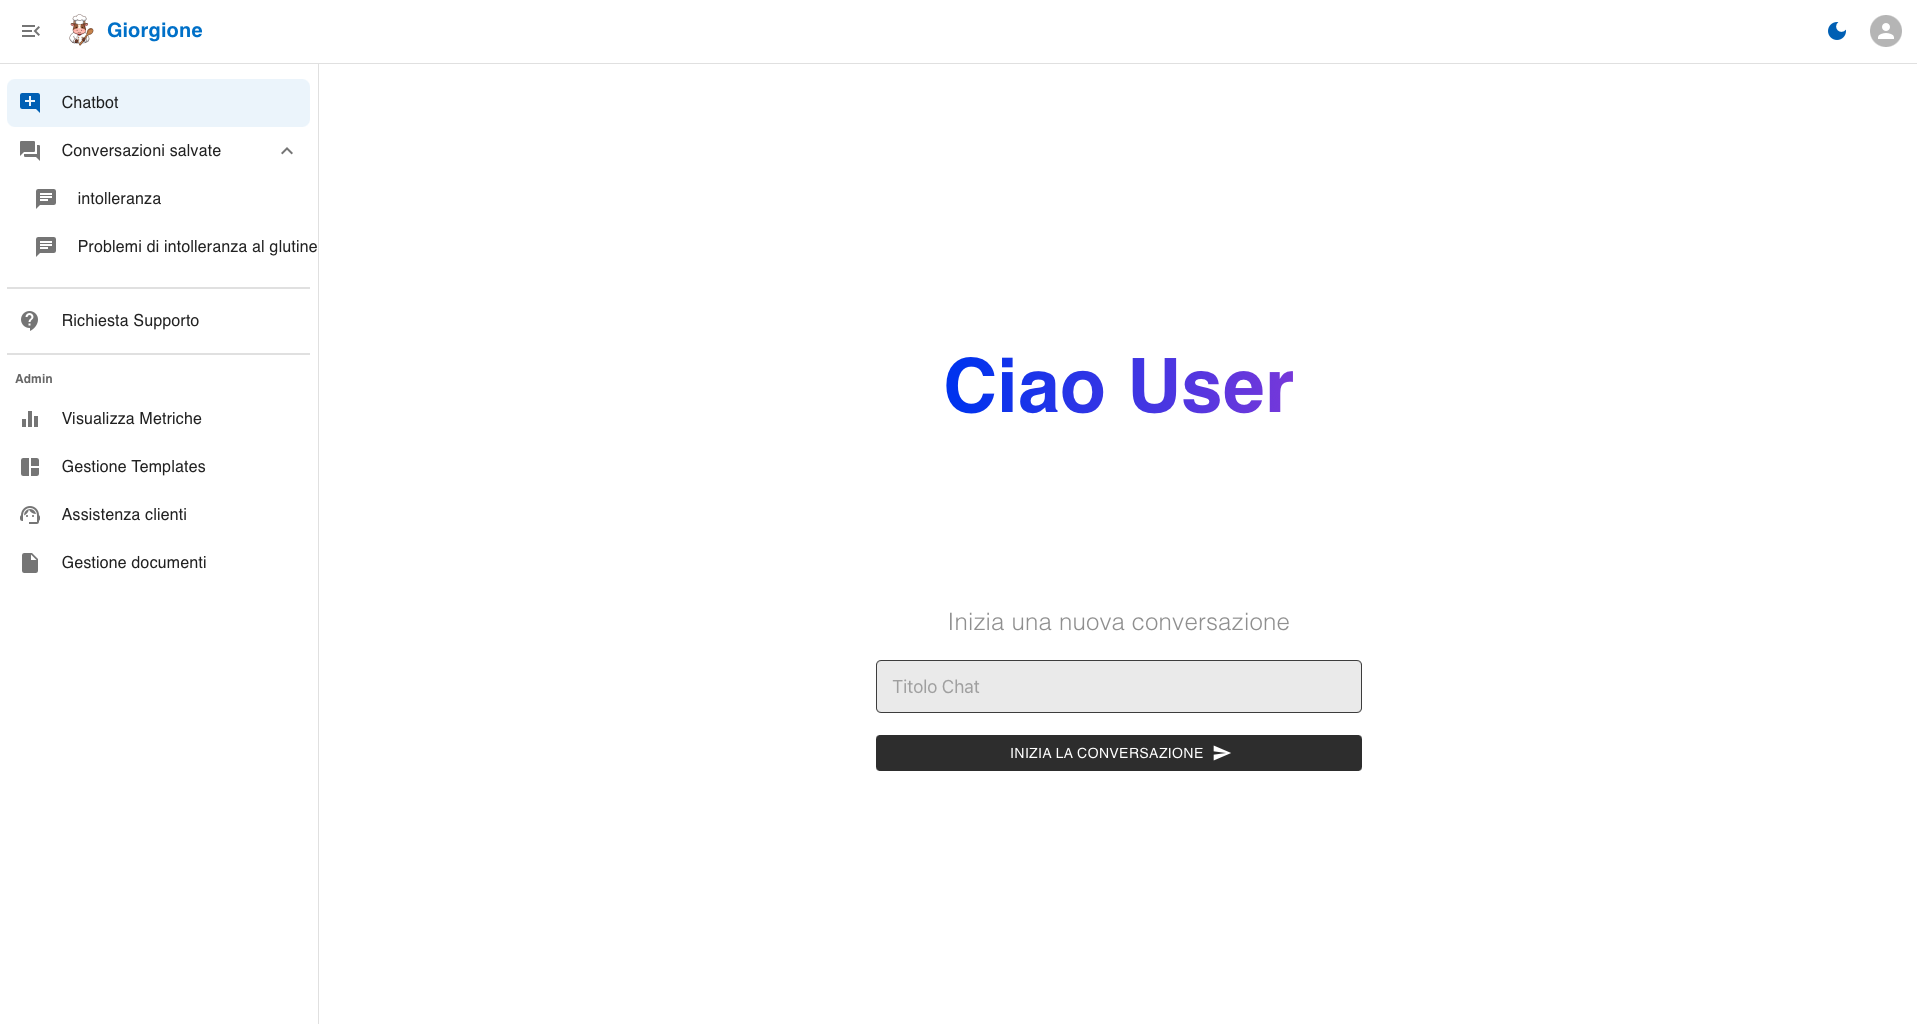
\includegraphics[width=0.8\textwidth]{./img/paginaIniziale.png}
%     \caption{Schermata della pagina di registrazione}
% \end{figure}

% \subsubsection{Schermata di conversazione}
% Una volta creata la conversazione dalla schermata iniziale l'utente può andare nel menù laterale (\textit{nel caso esso sia chiuso si può aprire tramite menù ad hamburger}) e selezionare la voce: "\textit{Conversazioni salvate}" che aprirà un menù a tendina dove l'utente potrà selezionare la conversazione desiderata.
% \begin{figure}[h!]
%     \centering
%     \begin{subfigure}{0.3\textwidth}
%         \centering
%         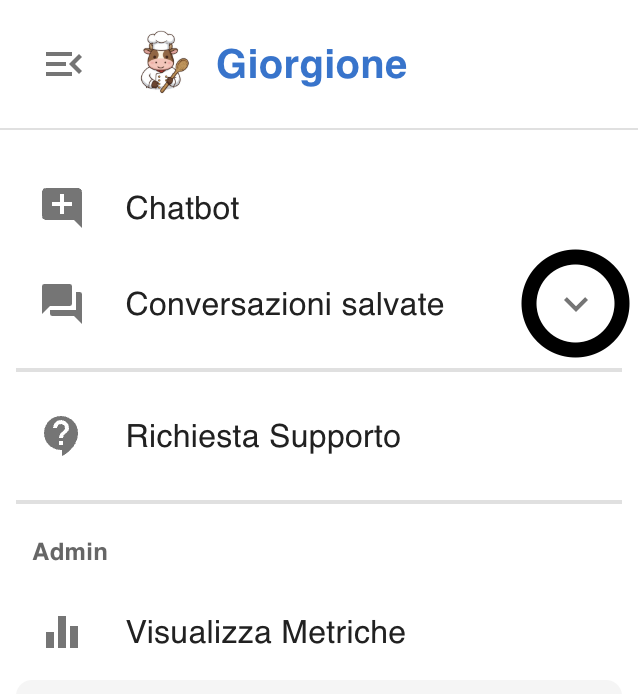
\includegraphics[width=\textwidth]{./img/laterale1.png}
%     \end{subfigure}
%     \hspace{0.05\textwidth}
%     \begin{subfigure}{0.3\textwidth}
%         \centering
%         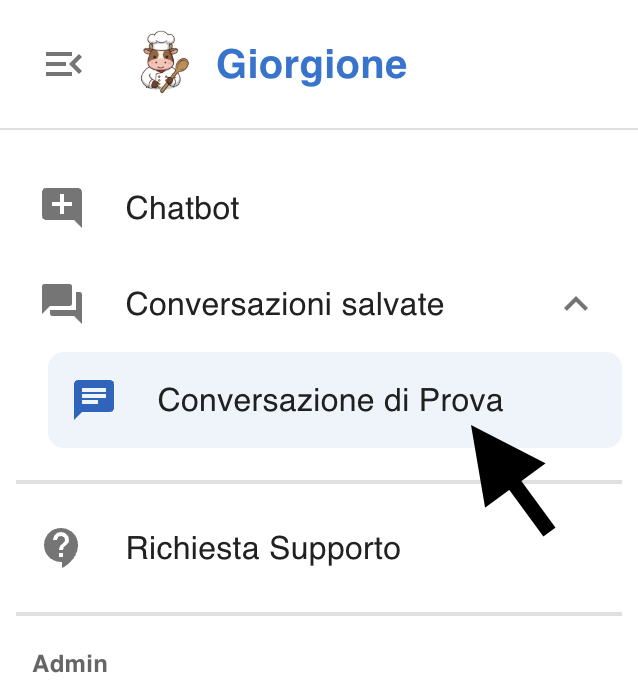
\includegraphics[width=\textwidth]{./img/laterale2.png}
%     \end{subfigure}
%     \caption{Menù laterale}
% \end{figure}
% L'utente si trovera quindi di fronte a una schermata composta da diversi elementi:
% \begin{figure}[h!]
%     \centering
%     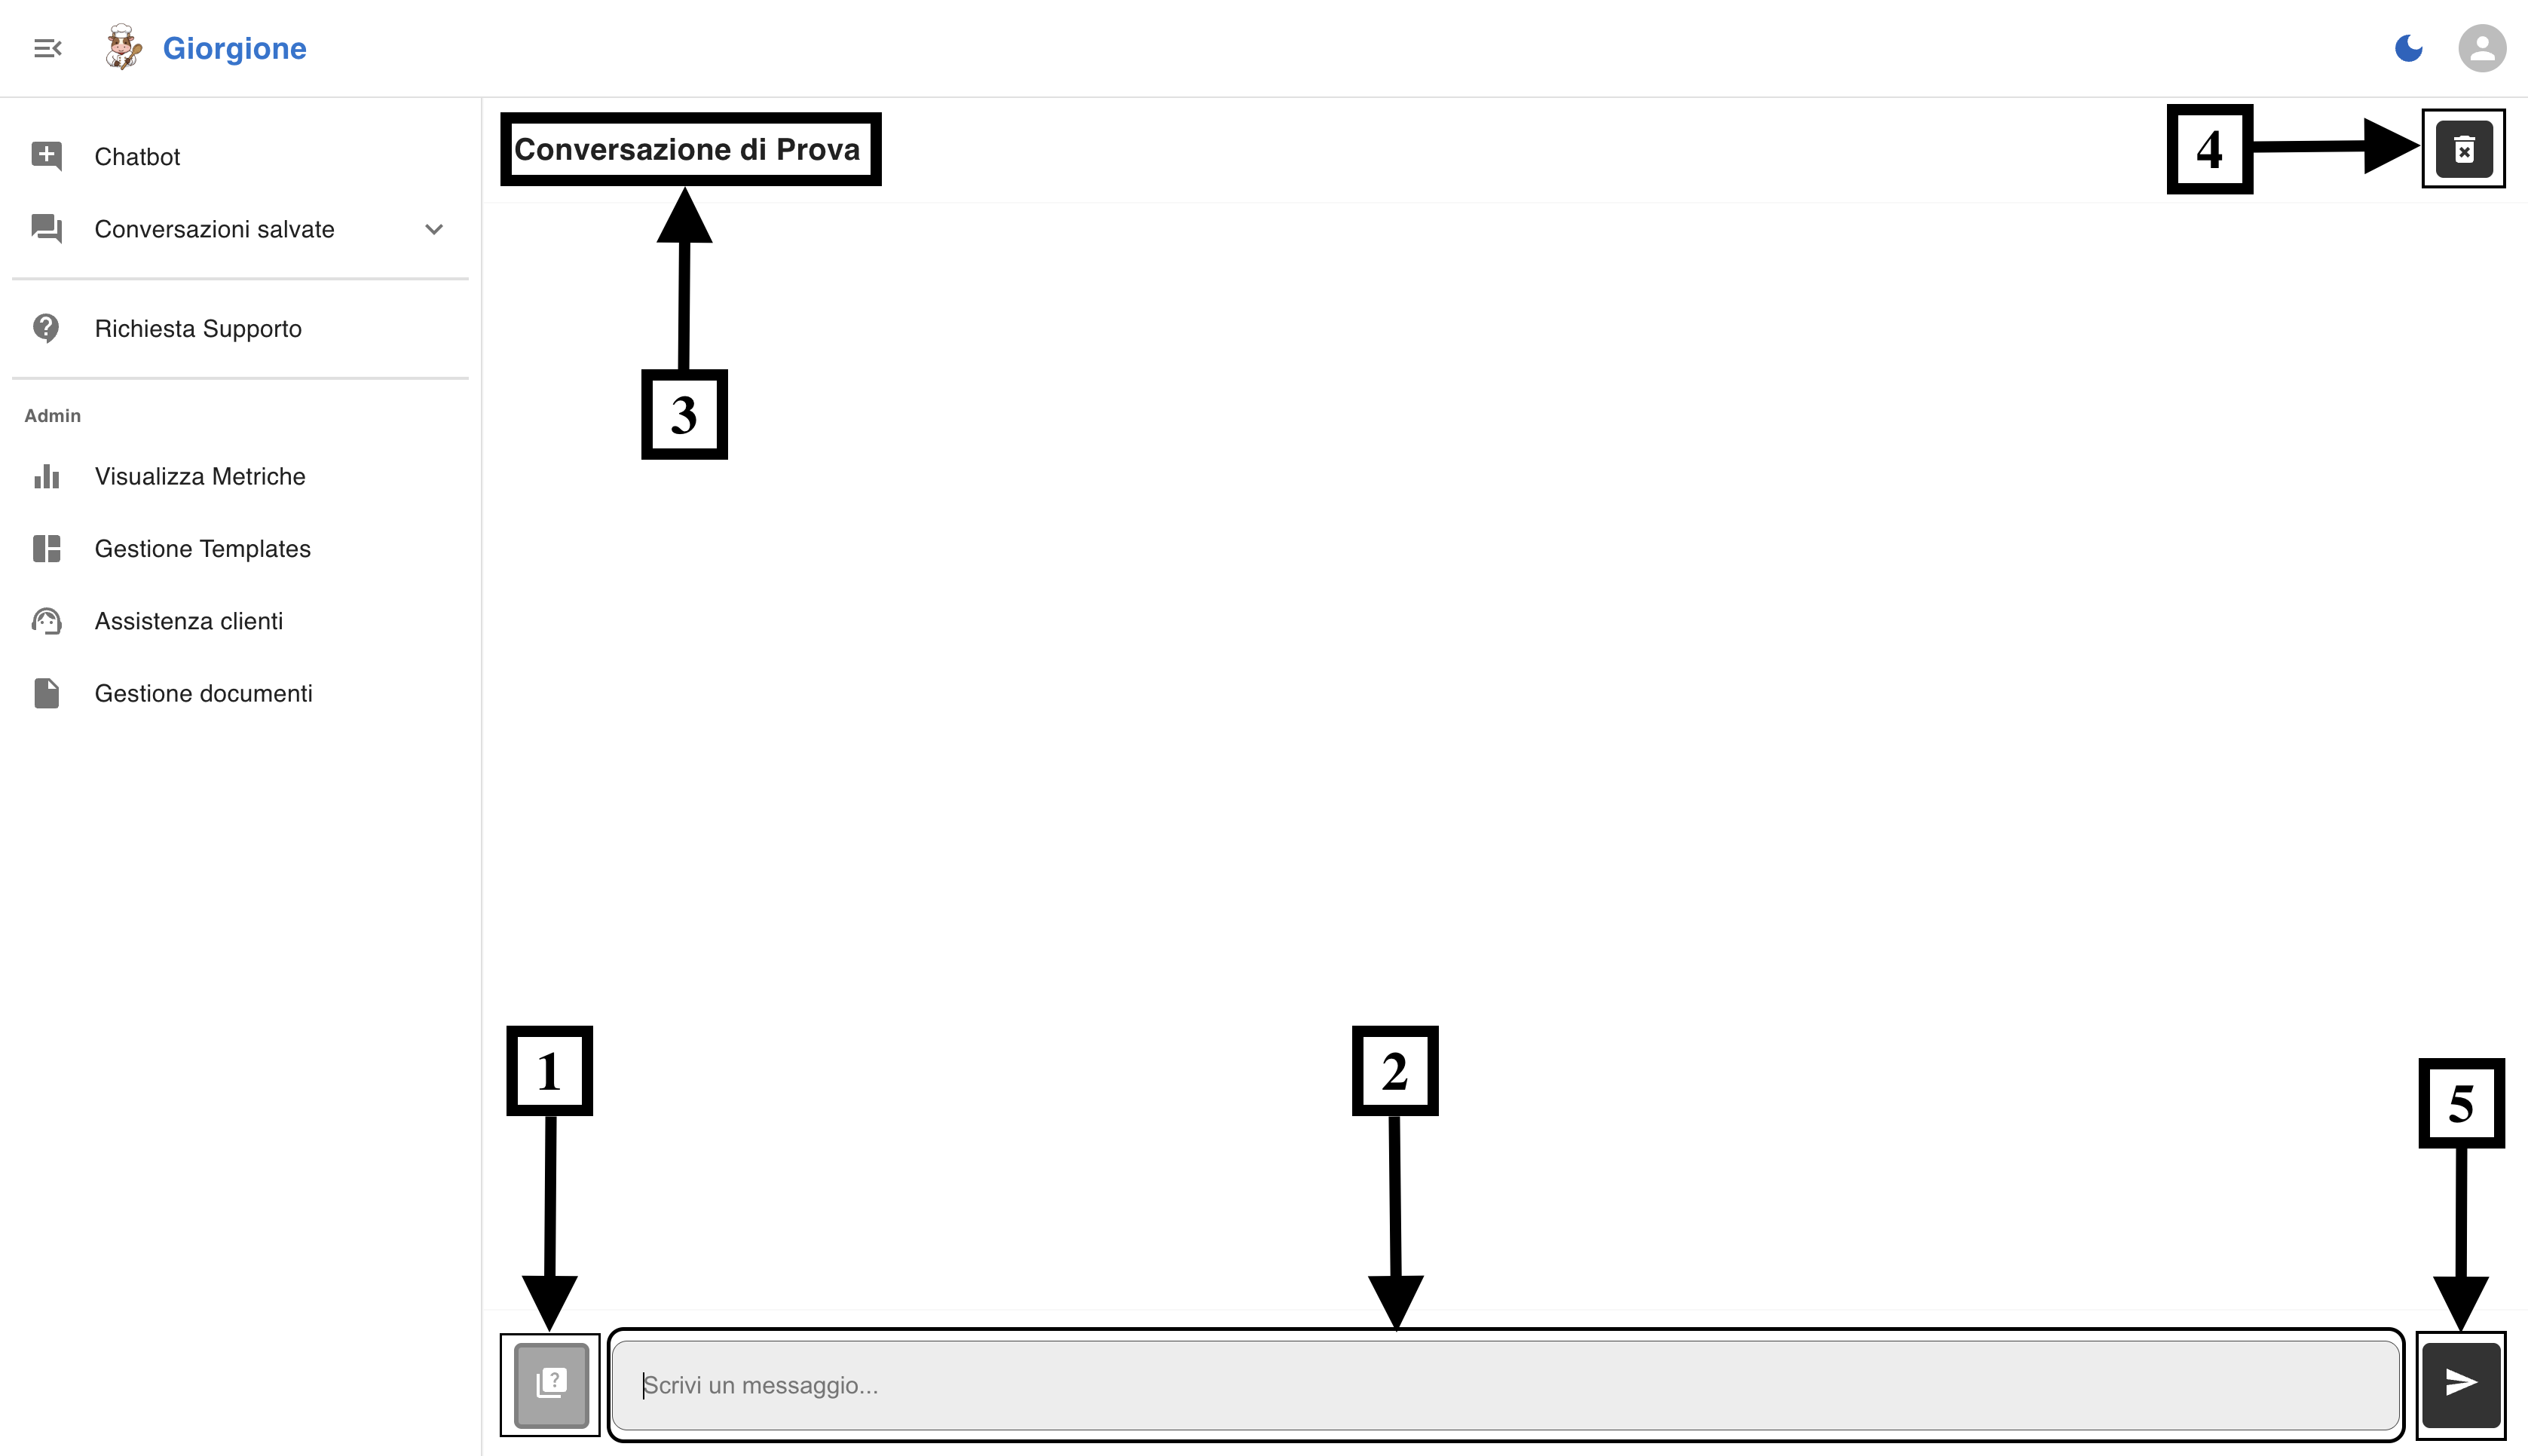
\includegraphics[width=\textwidth]{./img/SchermataChat1.png}
%     \caption{Schermata della chat}
%     \label{fig:schermata-chat}
% \end{figure}
% \newpage
% Facendo riferimento alla figura~\ref{fig:schermata-chat} infatti l'utente troverà un bottone per selezionare una domanda templetizzata (\textit{qui segnato con il numero 1}), cliccato il bottone sarà presente selezionare la domanda e inviarla all'assistente virtuale come mostrato in figura~\ref{fig:domanda templetizzata}.
% \begin{figure}[htbp]
%     \centering
%     \begin{tikzpicture}
%         % Inserisci le immagini
%         \node[anchor=east,inner sep=0] (img1) at (0,0) {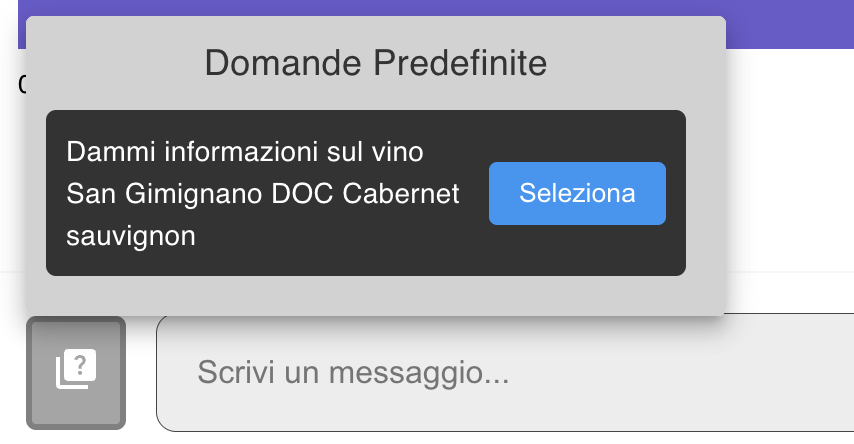
\includegraphics[width=0.4\textwidth]{img/SelettoreTemplate1.png}};
%         \node[anchor=west,inner sep=0] (img2) at (2,0) {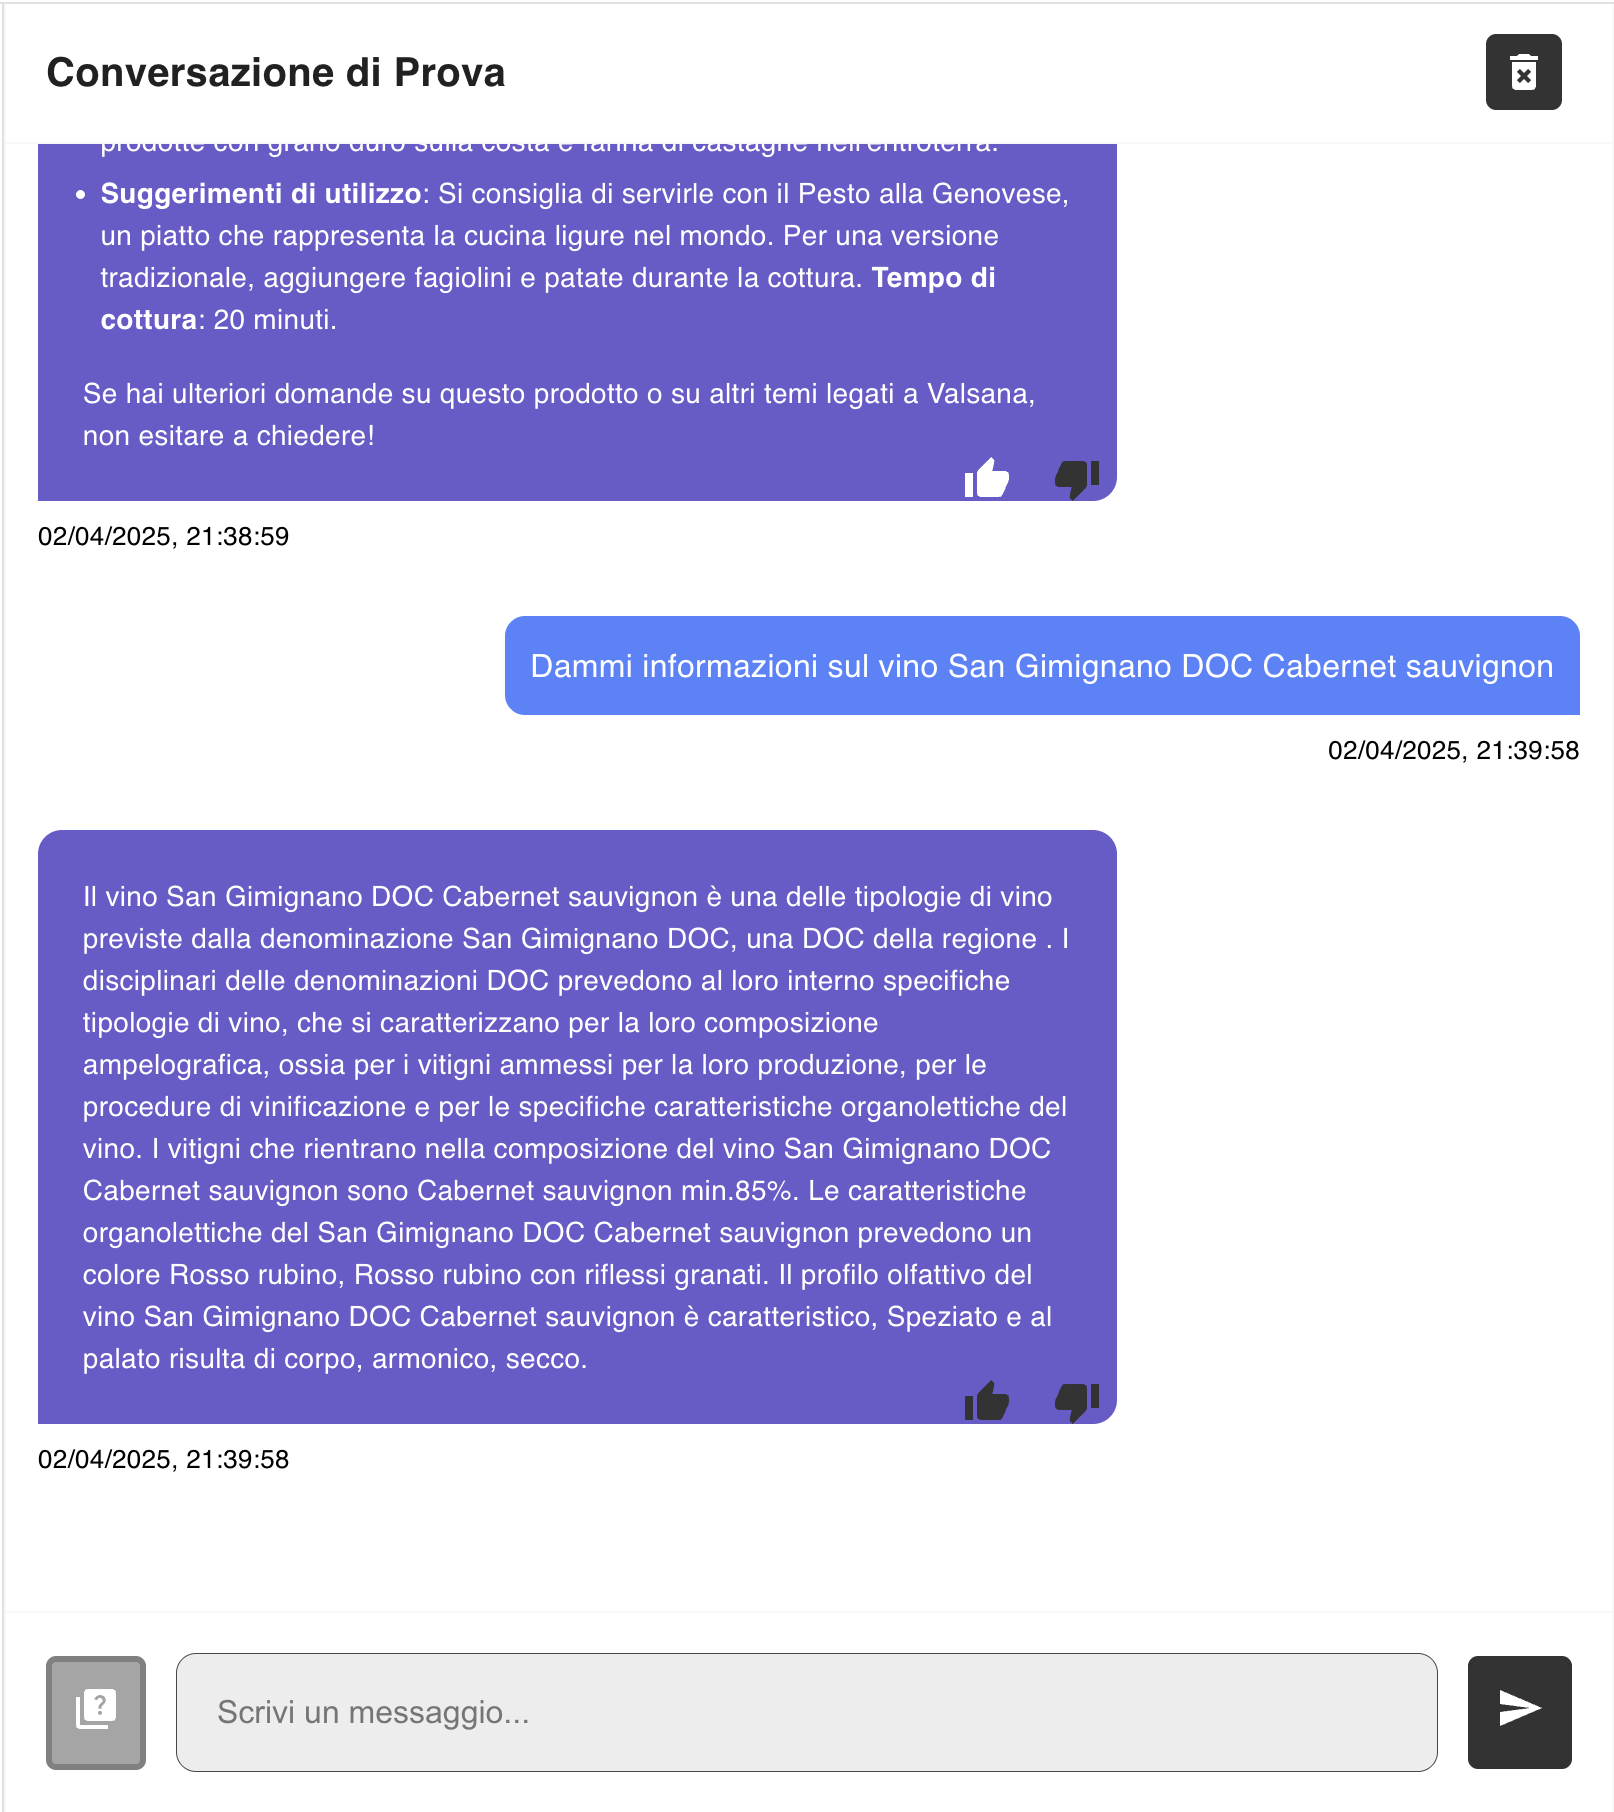
\includegraphics[width=0.4\textwidth]{img/SelettoreTemplate2.png}};
        
%         % Disegna una freccia
%         % Disegna una freccia dritta orizzontale
%         \draw[->, thick] (img1.east) -- (img2.west);
%         \end{tikzpicture}
%         \caption{Seleziona domanda templetizzata}
%         \label{fig:domanda templetizzata}
% \end{figure}
% \\
% Il punto numero 2 indica invece la casella di testo dove l'utente potrà scrivere il proprio messaggio da inviare al bot.
% Il punto numero 3 indica il nome della conversazione precedentemente scelto nella schermata iniziale. Il punto numero 4 indica un bottone che permette di eliminare la chat premendolo apparirà un pop-up che chiede cortesemente all'utente se è sicuro di voler eliminare la conversazione figura~\ref{fig:elimina-chat}:
% \begin{figure}[h!]
%     \centering
%     
\includegraphics[width=0.5\textwidth]{./img/eliminaChat.png}
%     \caption{Elimina chat}
%     \label{fig:elimina-chat}
% \end{figure}
% \\
% Il punto numero 5 in figura~\ref{fig:schermata-chat} è il pulsante invio che permette di mandare un messaggio al nostro assistente virtuale. Bisogna dire tuttavia che è possibile inviare un messaggio solo se del testo è presente nella casella di testo (\textit{punto 2 in figura~\ref{fig:schermata-chat}}) e che non è necessario cliccare sul pulsante in quanto è possibile premere direttamente invio sulla tastiera.
% \\
% Inviato un messaggio questo apparirà nella parte destra della schermata come avviene nelle più famose chat di messaggistica (fare riferimento a figura~\ref{fig:Elaborazione} punto 6), e verrà mostrato il messaggio e la data e l'ora dell'invio.
% Nella parte sinistra l'utente potrà osservare il nostro Assistente virtuale Giorgione elaborare il messaggio per soddisfare la richiesta dell'utente (punto 7 figura~\ref{fig:Elaborazione}).
% \begin{figure}[h!]
%     \centering
%     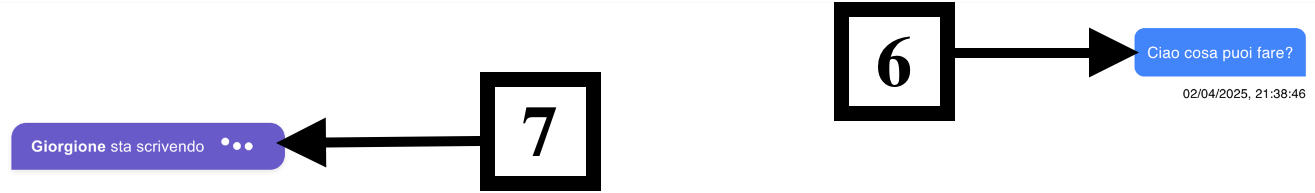
\includegraphics[width=\textwidth]{./img/SchermataChat2.png}
%     \caption{Elaborazione del messaggio}
%     \label{fig:Elaborazione}
% \end{figure}
% \\
% Una volta mandato il messaggio esso sarà visualizzabile come mostrato in figura~\ref{fig:Visualizzazione Risposta} punto 8, e l'utente potrà decidere opzionalmente se è soddisfatto della risposta data dal bot di fornire una valutazione booleana indicata da un pollice in su e pollice in giù (\textit{figura~\ref{fig:Visualizzazione Risposta} punto 9}):
% \begin{figure}[h!]
%     \centering
%     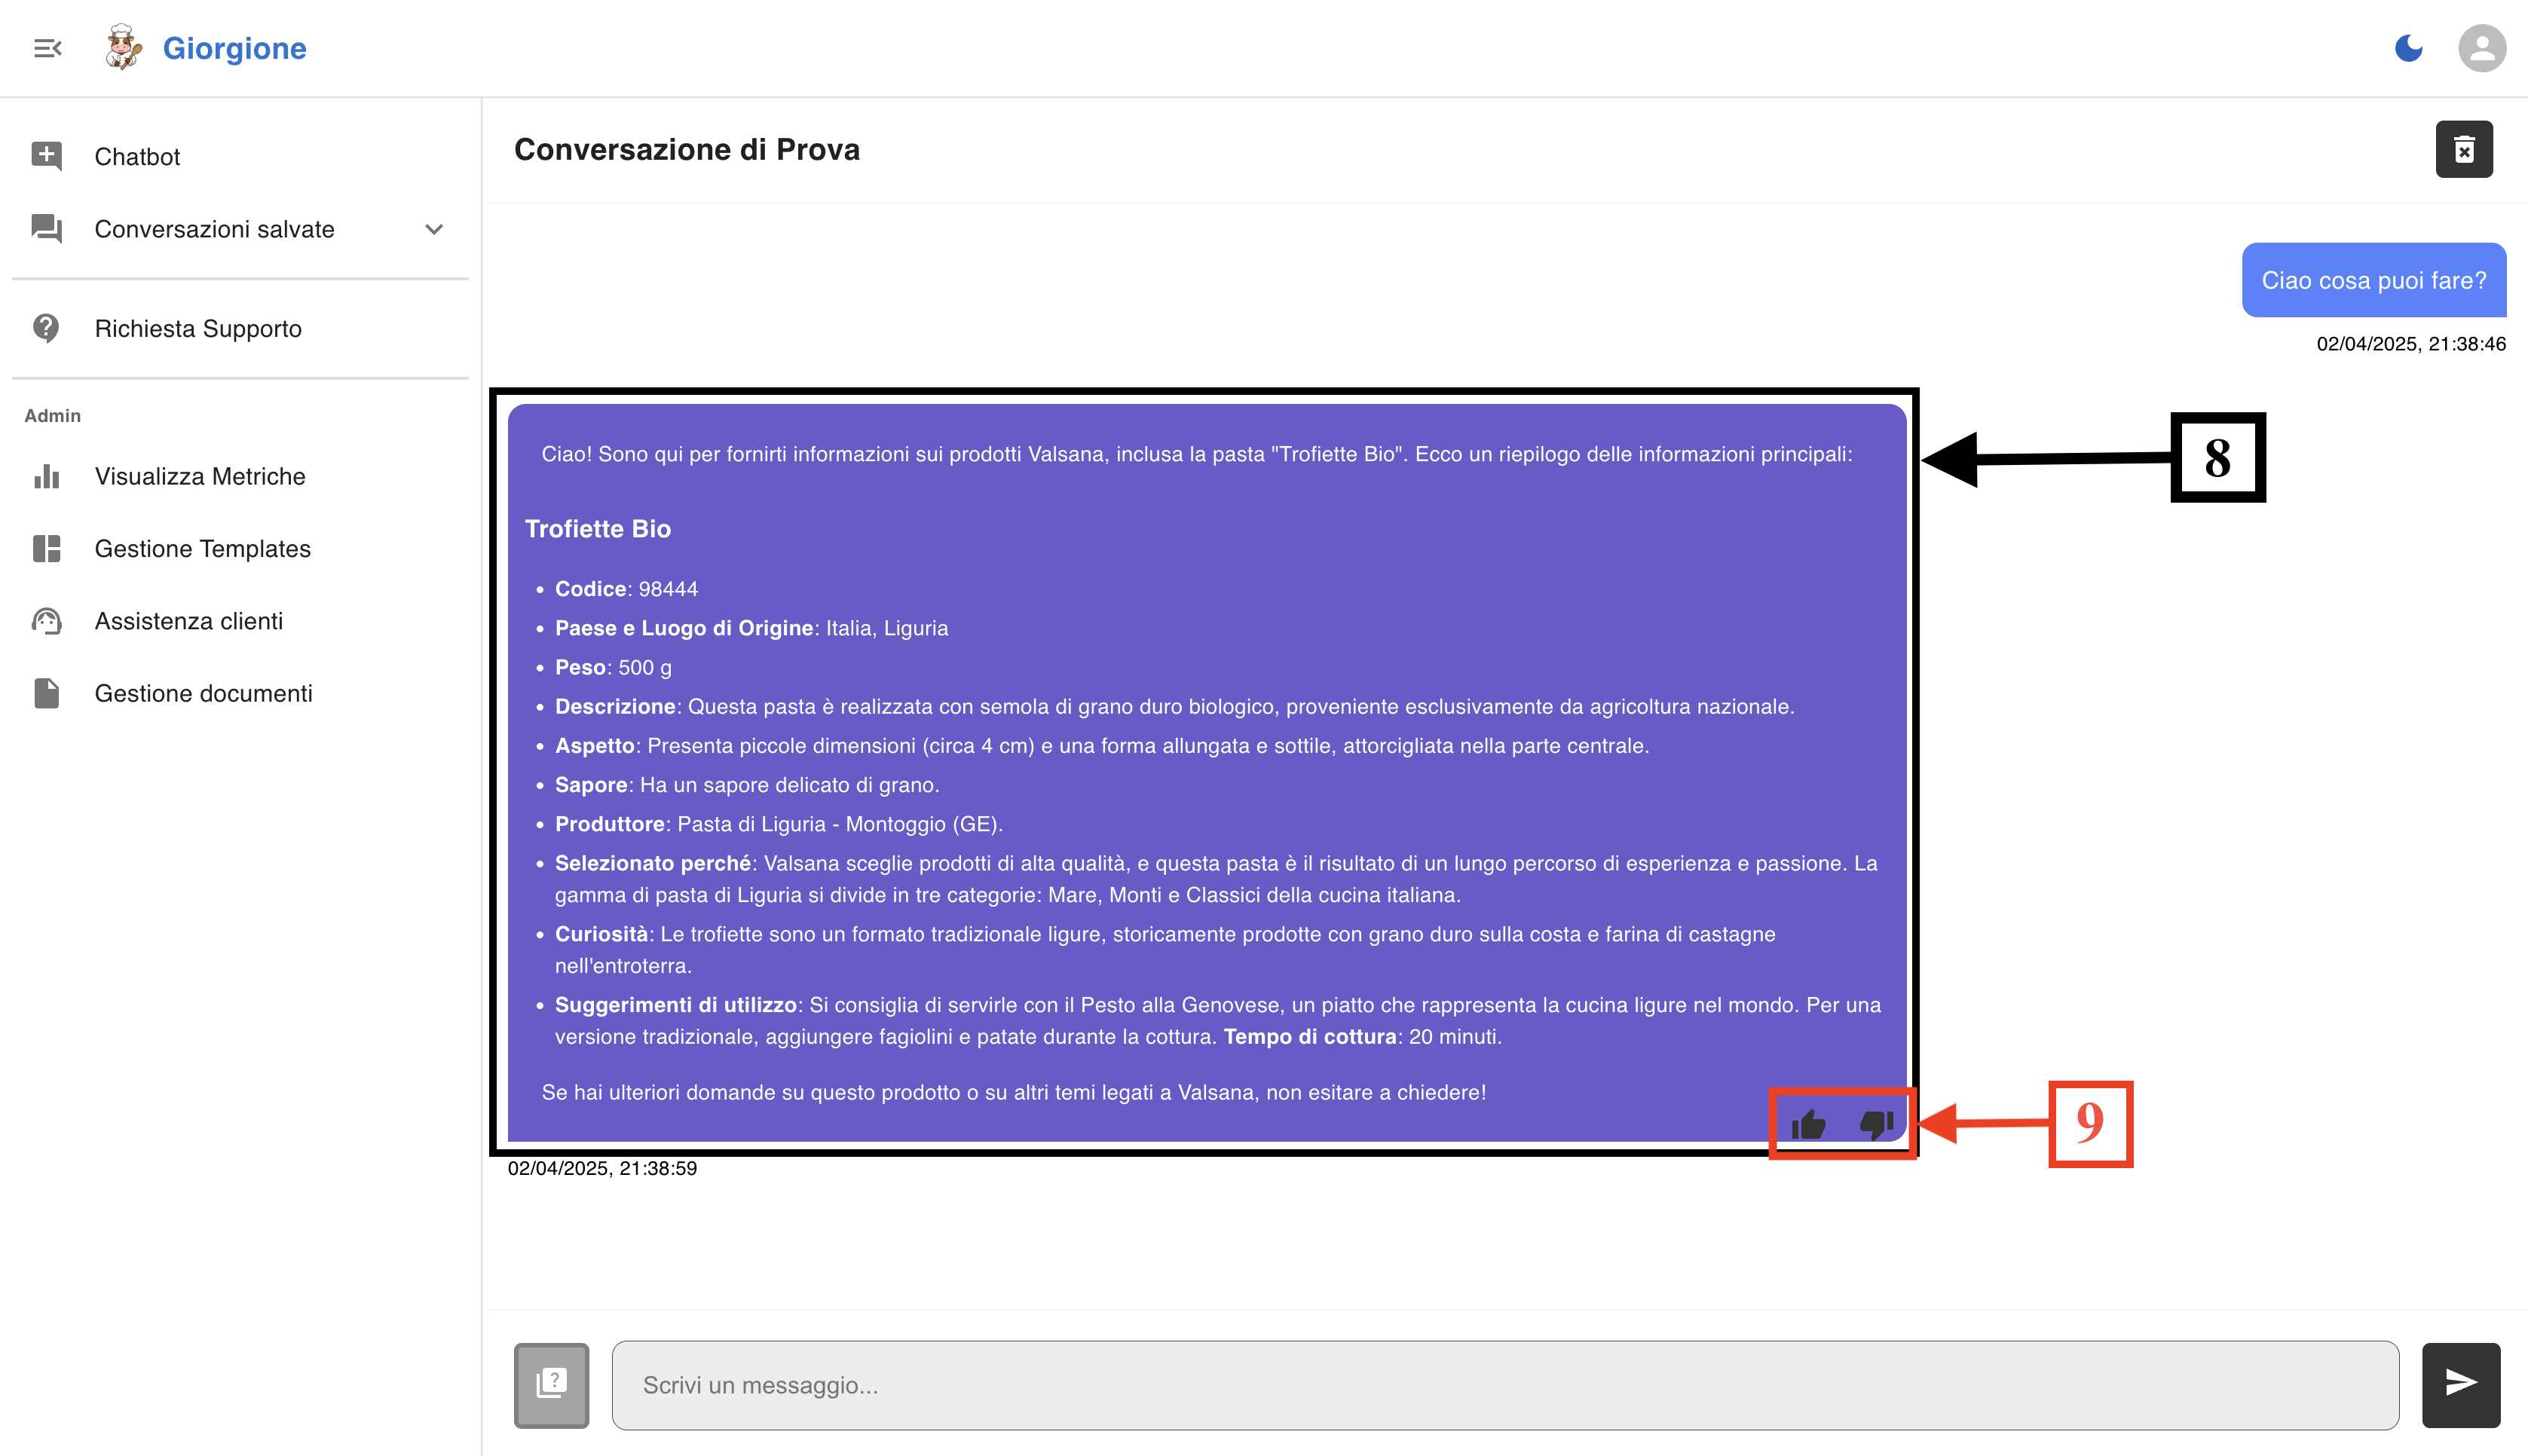
\includegraphics[width=\textwidth]{./img/SchermataChat3.png}
%     \caption{Visualizzazione Risposta}
%     \label{fig:Visualizzazione Risposta}
% \end{figure}
% L'utente è notificato dalla scelta dall'illuminazione di uno dei 2 bottoni come mostrato in figura~\ref{fig:likedislike}
% \begin{figure}[h!]
%     \centering
%     \begin{subfigure}{0.2\textwidth}
%         \centering
%         
\includegraphics[width=\textwidth]{./img/like.png}
%         \caption{Caso in cui l'utente scelga like}
%     \end{subfigure}
%     \hspace{0.05\textwidth}
%     \begin{subfigure}{0.2\textwidth}
%         \centering
%         
\includegraphics[width=\textwidth]{./img/dislike.png}
%         \caption{Caso in cui l'utente scelga dislike}
%     \end{subfigure}
%     \caption{Feedback Risposta}
%     \label{fig:likedislike}
% \end{figure}

% \newpage

% \subsubsection{Pagina di Richiesta di Supporto}
% Selezionando dal menù laterale la voce "Richiesta Supporto" (fig~\ref{fig:Pagina di Assistenza} pt.1). L'utente si troverà davanti ad una pagina dove potrà inviare un messaggio all'admin in caso di problemi.
% Una richiesta dovrà essere composta da un Oggetto inseribile nella casella di testo (fig~\ref{fig:Pagina di Assistenza} pt.2), una descrizione (fig~\ref{fig:Pagina di Assistenza} pt.3).\\
% Una volta compilati l'utente può inviare il messaggio cliccando sul bottone invia indicato in fig~\ref{fig:Pagina di Assistenza} pt.4, e successivamente verrà notificato dell'invio riuscito o non riuscito come mostrato in fig~\ref{fig:InvioRiuscito} (\textit{Ci riserviamo di mostrare solo l'invio riuscito}).
% \begin{figure}[h!]
%     \centering
%     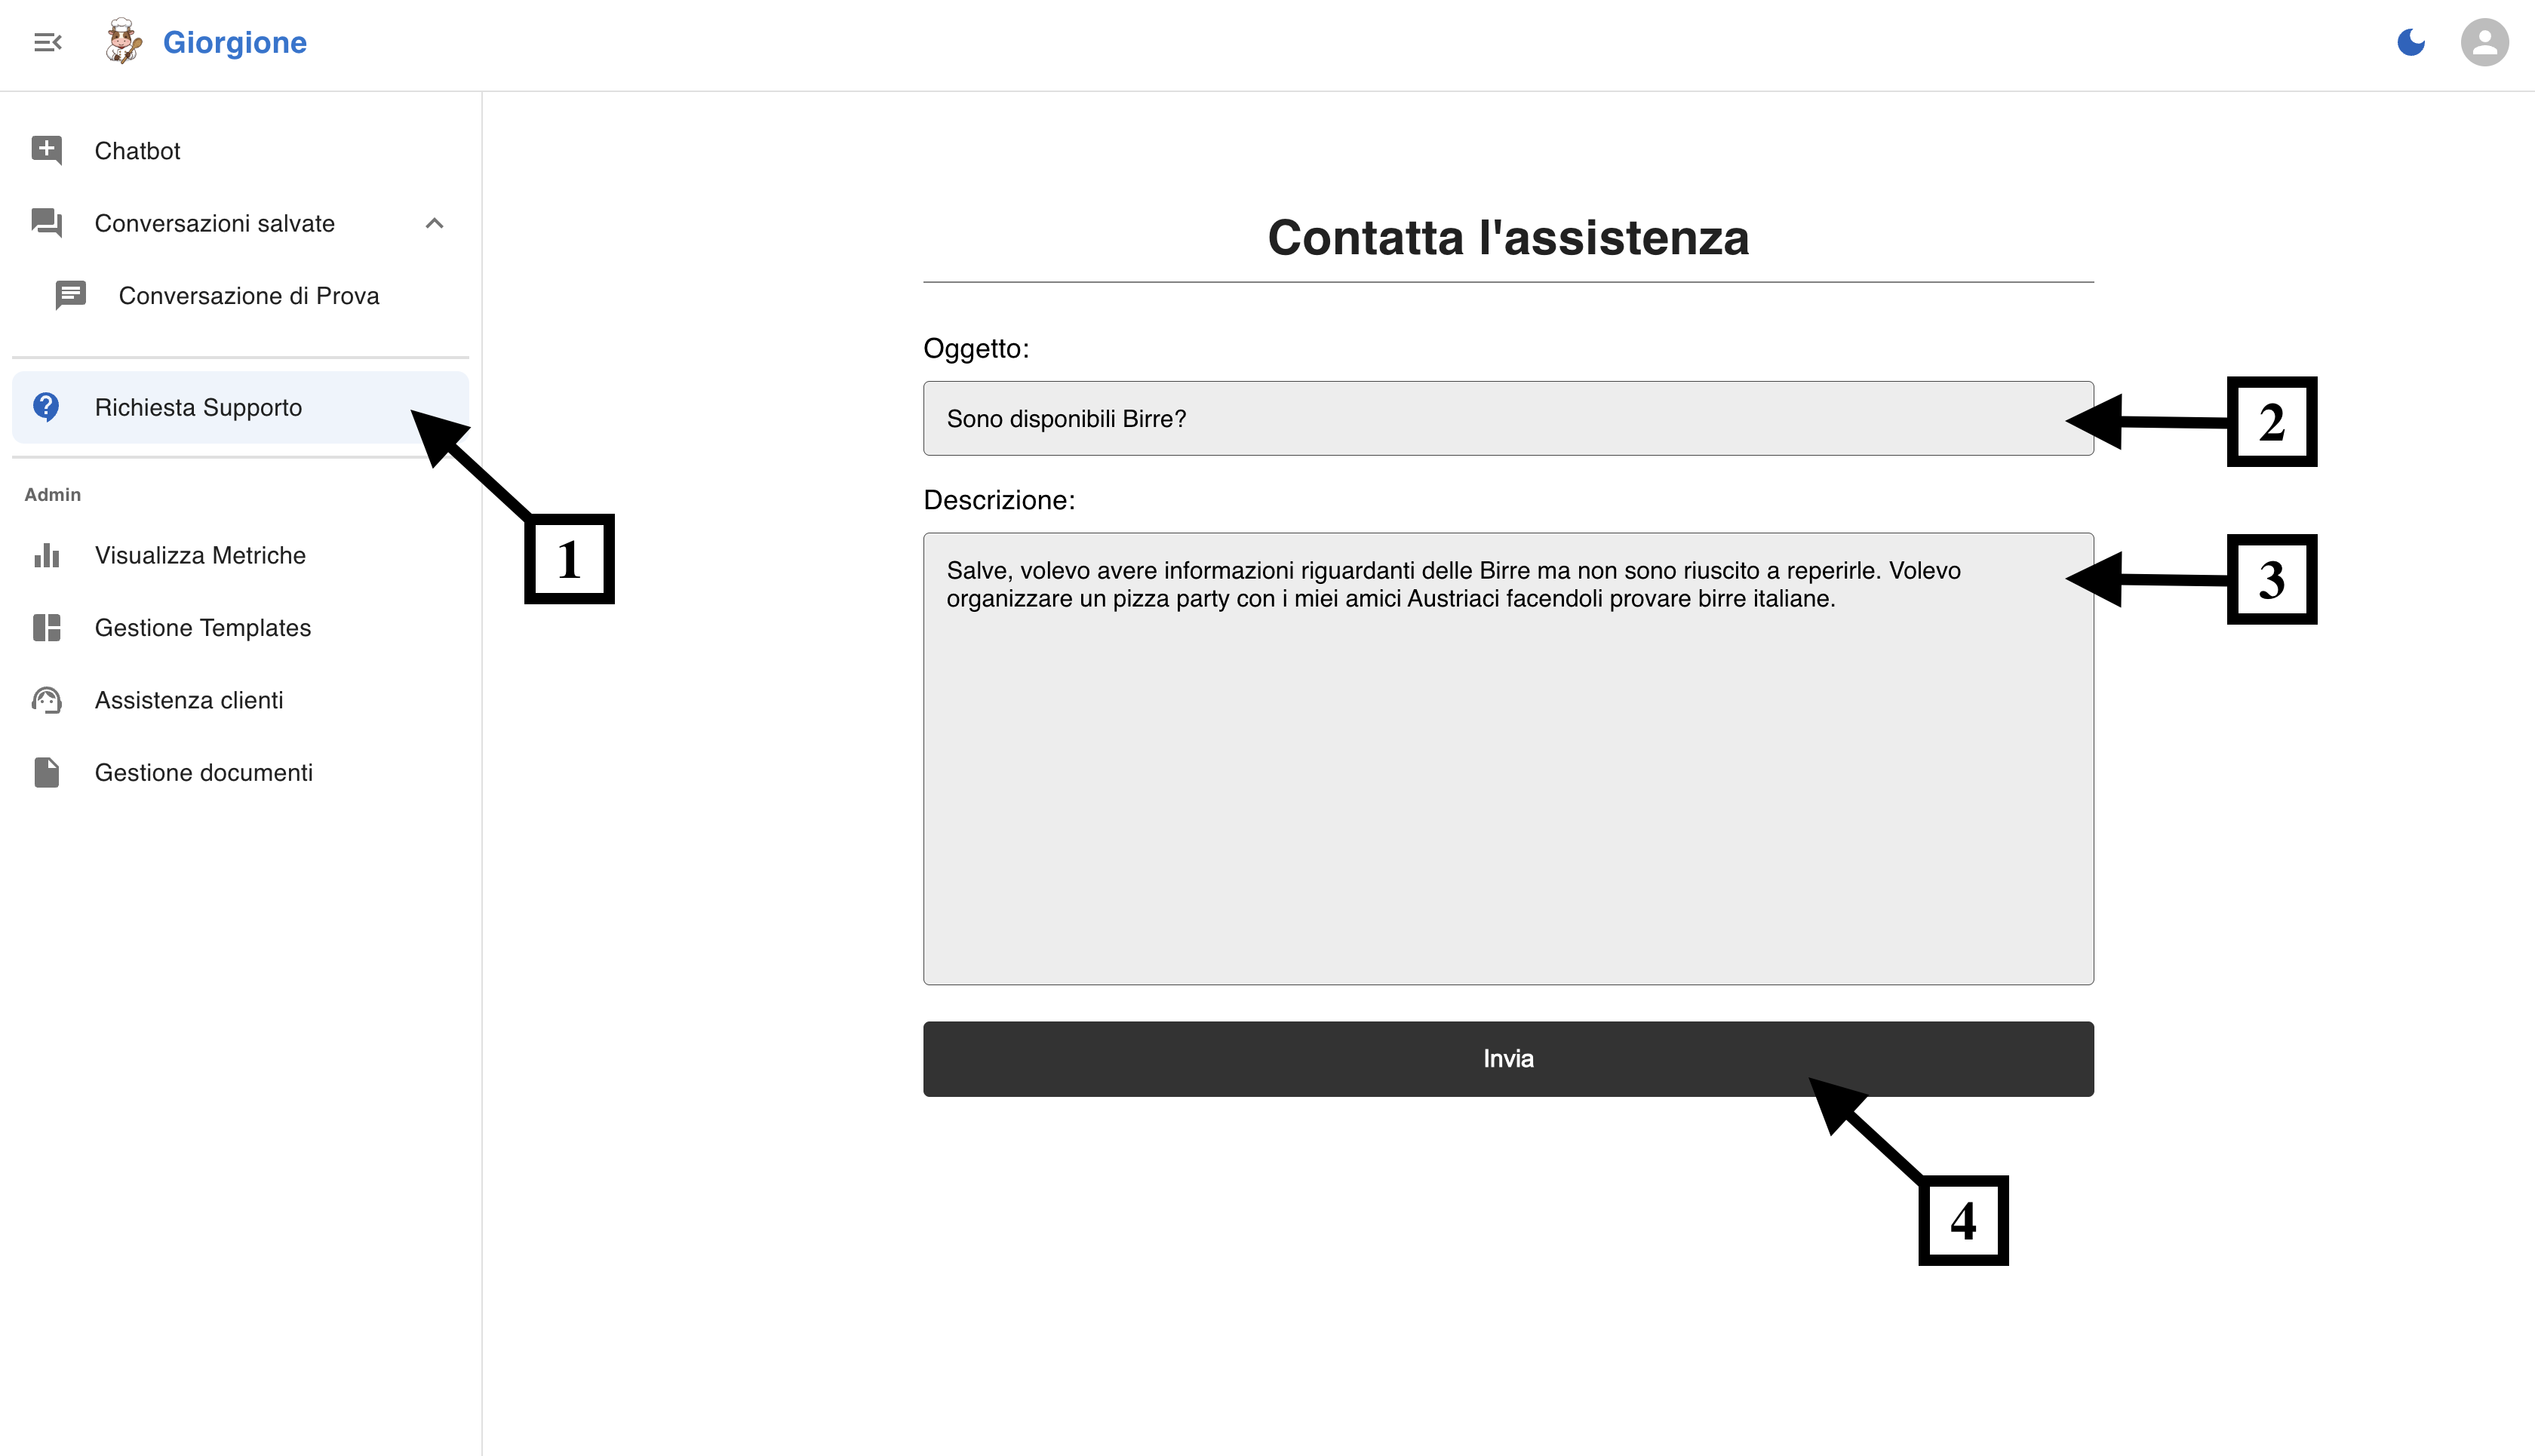
\includegraphics[width=\textwidth]{./img/RichiestaAssistenza1.png}
%     \caption{Pagina di Assistenza}
%     \label{fig:Pagina di Assistenza}
% \end{figure}
% \begin{figure}[h!]
%     \centering
%     
\includegraphics[width=0.8\textwidth]{./img/RichiestaAssistenza2.png}
%     \caption{Invio Richiesta Assistenza Riuscita}
%     \label{fig:InvioRiuscito}
% \end{figure}

% \subsubsection{Logout}
% Cliccando in alto a destra su qualsiasi schermata sarà possibile cliccare sull'icona utente e premere sul pulsante di sign out per tornare alla schermata di login.
% \begin{figure}[h!]
%     \centering
%     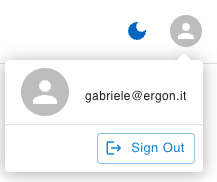
\includegraphics[width=0.3\textwidth]{./img/logout.png}
%     \caption{Logout}
% \end{figure}

% \subsection{Pagine riservate all'admin}
% In questa sezione mostriamo le pagine riservate all'admin.

% \subsubsection{Visualizza Metriche}
% L'admin cliccando dal menù laterale su Visualizza Metriche vedrà una Dashboard dove visualizzerà con valori numerici i like e i dislike delle conversazioni e il numero di messaggi totali gestiti dal Database.
% \begin{figure}[h!]
%     \centering
%     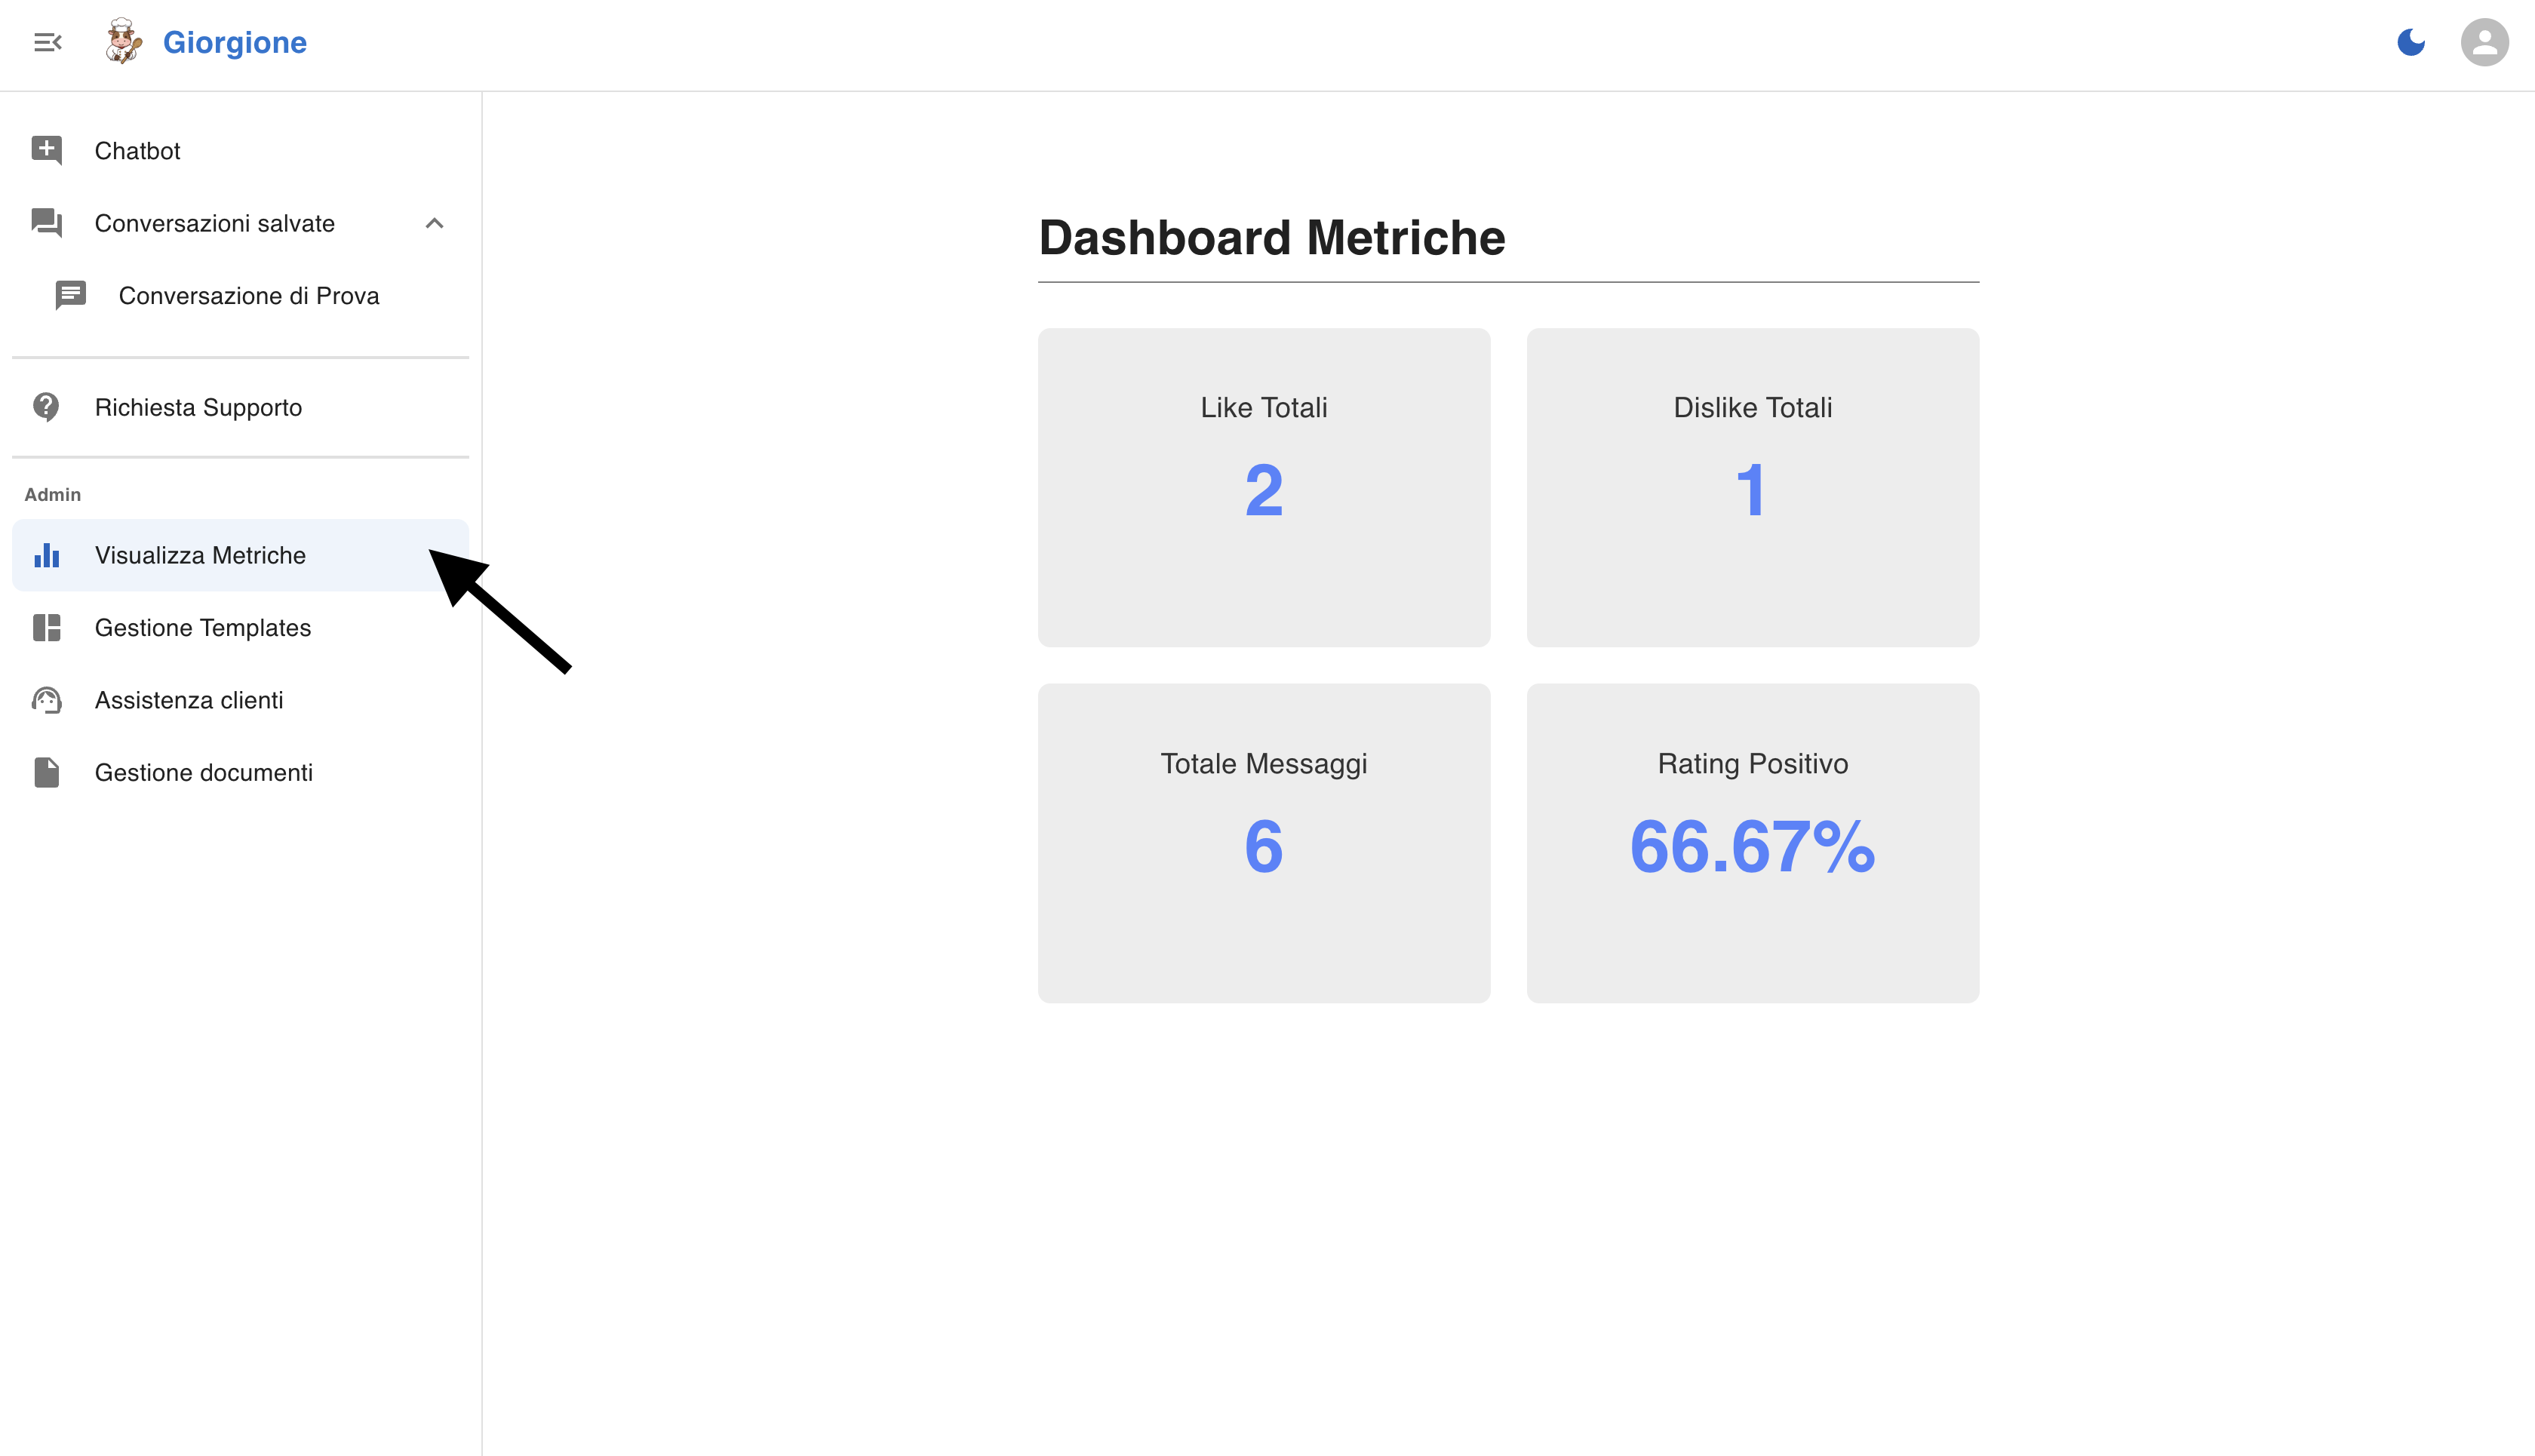
\includegraphics[width=\textwidth]{./img/visualizzaMetriche.png}
%     \caption{Dashboard Metriche}
%     \label{fig:Metriche}
% \end{figure}

% \subsubsection{Gestione Template}
% Selezionado dal menù laterale (fig~\ref{fig:Template} pt.1) accediamo alla pagina di gestione dei template. Qui è possibile visualizzare i template precedentemente inseriti dall'admin, aggiungerne di nuovi, modificarli ed eliminarli.
% \begin{figure}[h!]
%     \centering
%     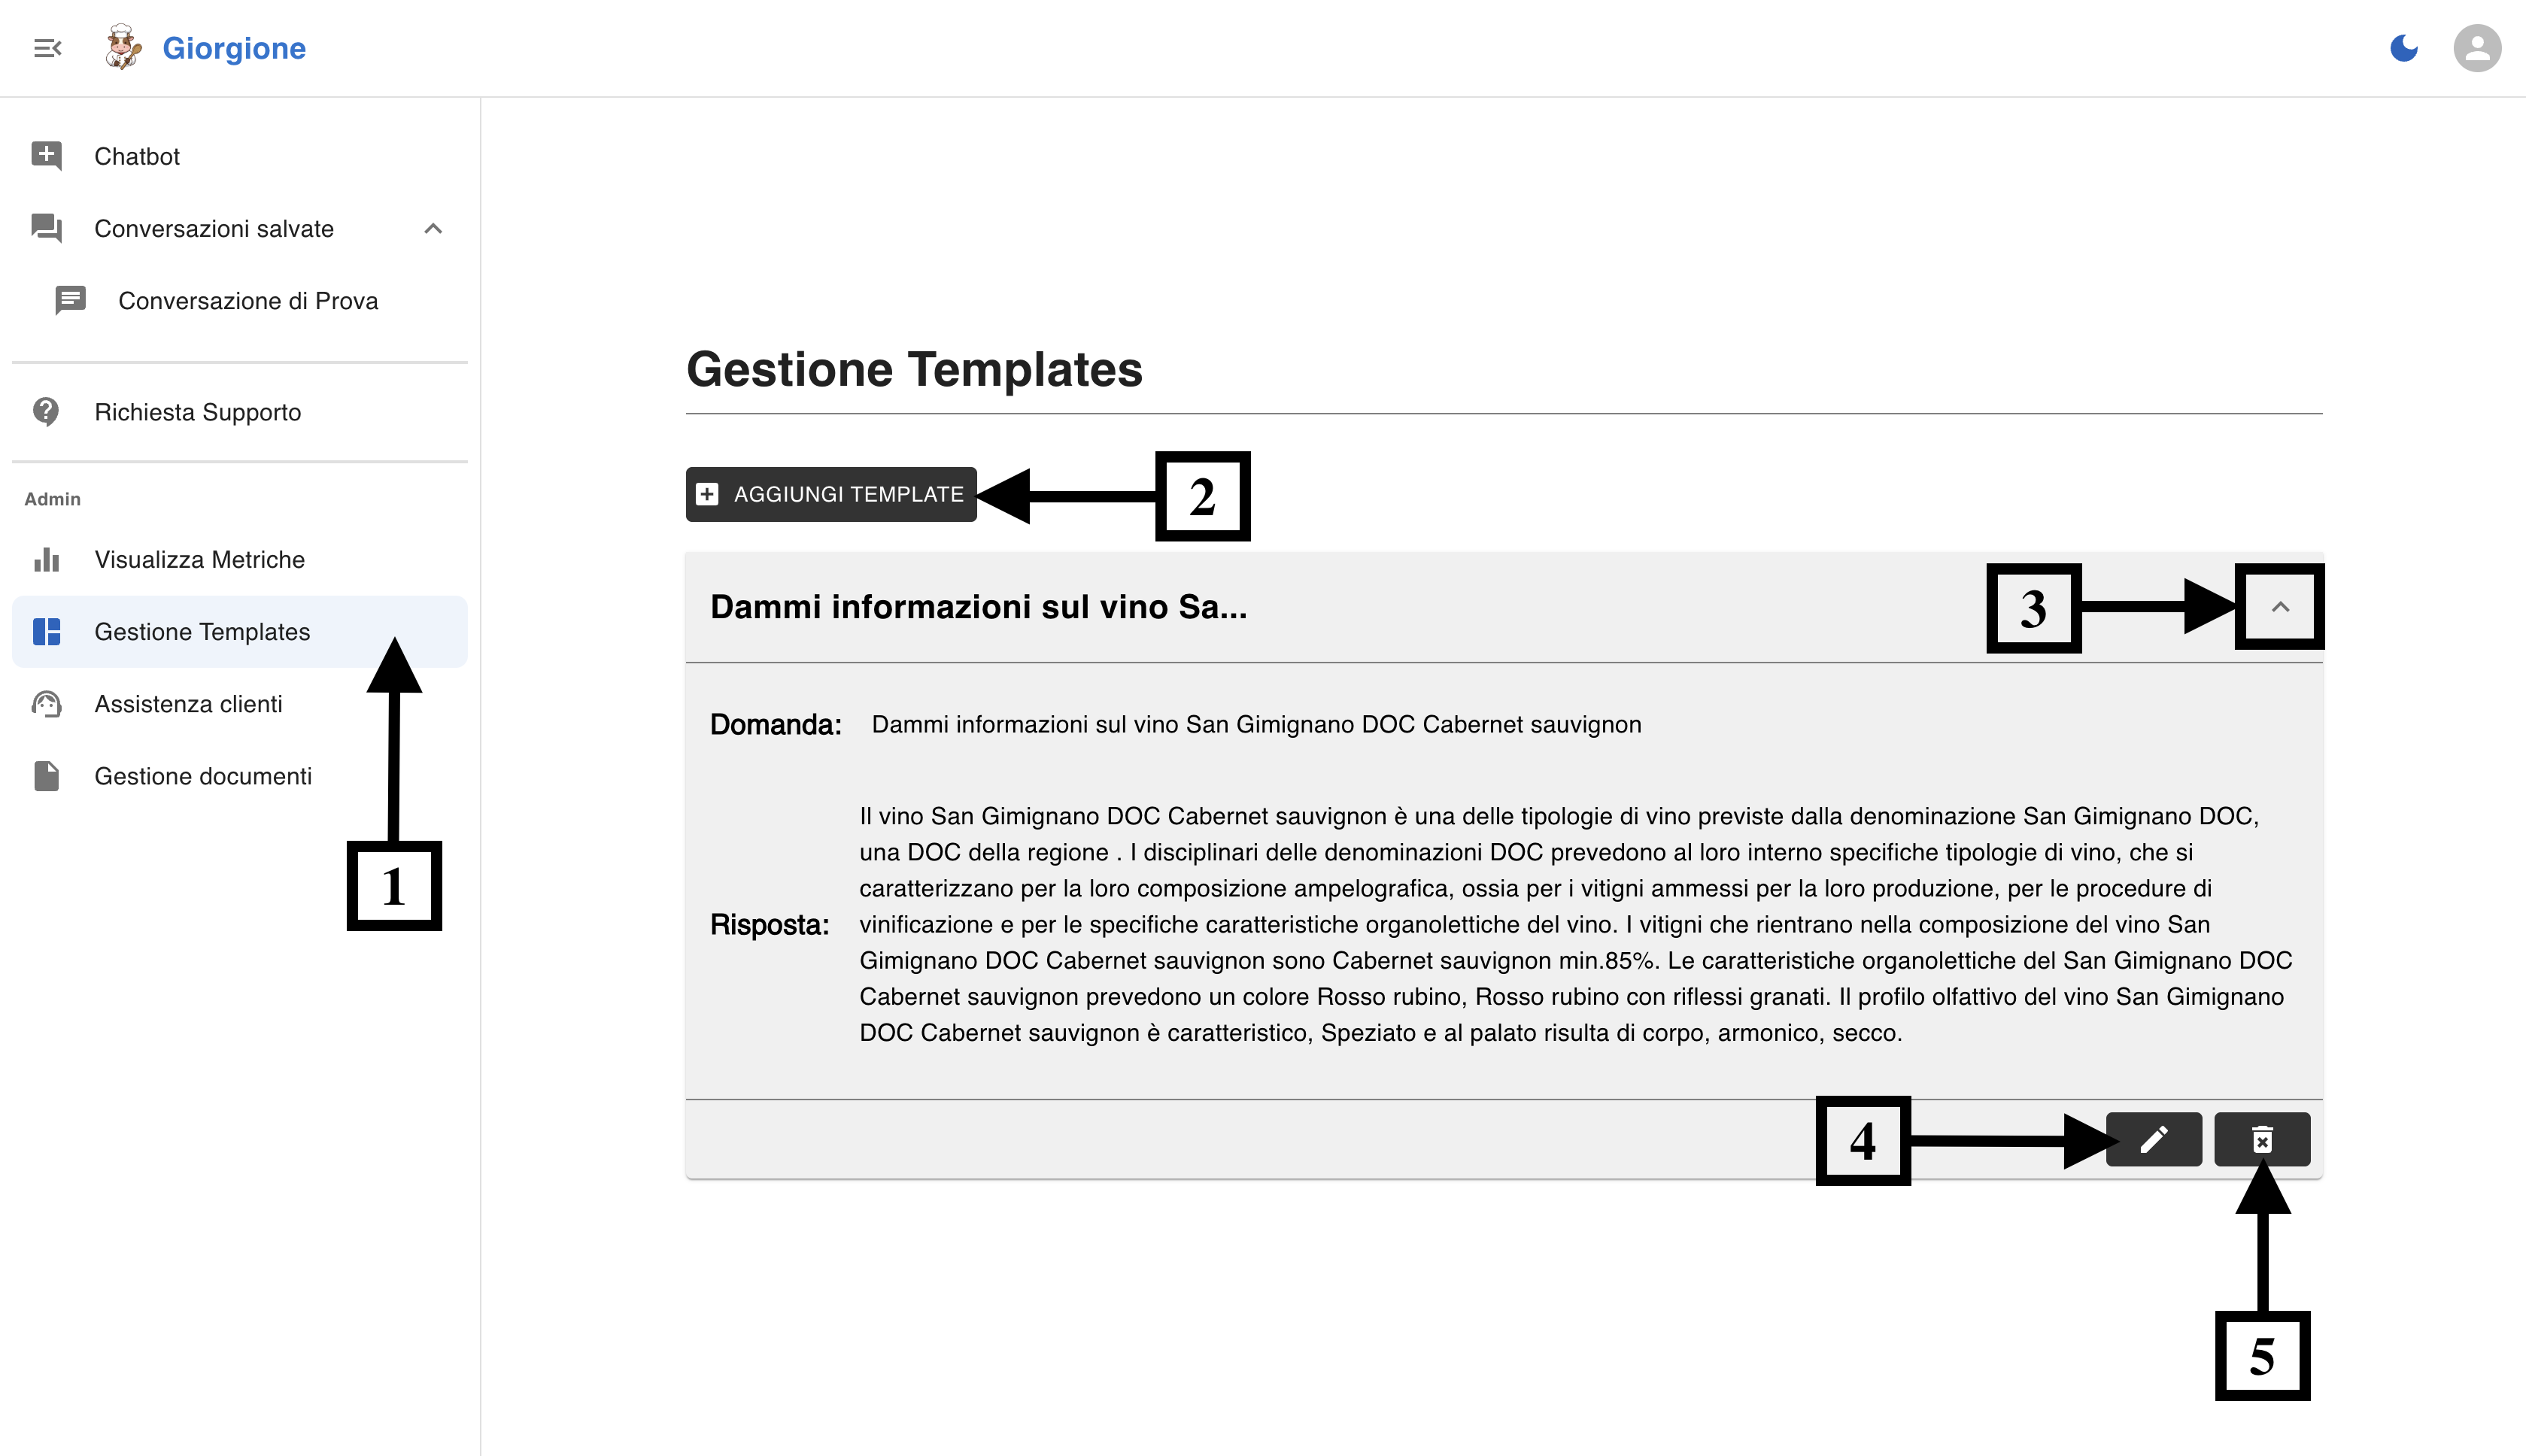
\includegraphics[width=\textwidth]{./img/GestioneTemplate.png}
%     \caption{Gestione Template}
%     \label{fig:Template}
% \end{figure}
% Per aggiungere un template basterà cliccare sul pulsante aggiungi template (fig~\ref{fig:Template} pt.2) che aprirà il pop-up mostrato in fig~\ref{fig:addTemplate} dove sarà possibile inserire la domanda e la risposta.
% \begin{figure}[h!]
%     \centering
%     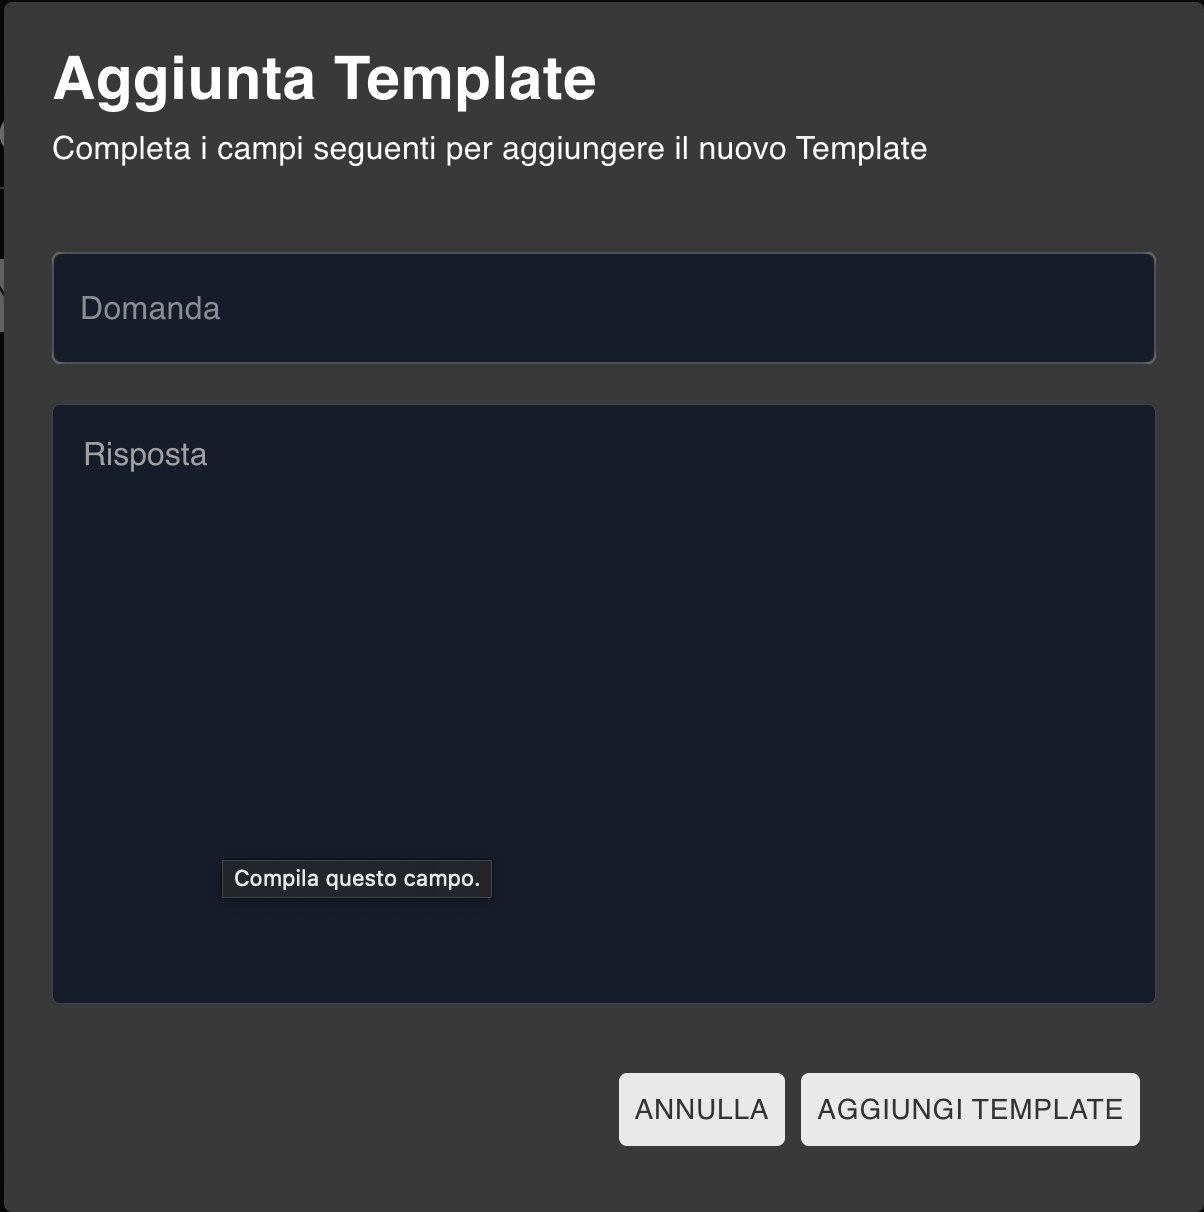
\includegraphics[width=0.4\textwidth]{./img/AggiungiTemplate.png}
%     \caption{Aggiungi Template}
%     \label{fig:addTemplate}
% \end{figure}
% Per visualizzare l'intero template e non solo il nome è possibile cliccare sul bottone mostrato in fig~\ref{fig:Template} pt.3 che aprirà una tendina dove verrà visualizzata l'intera domanda e l'intera risposta. Verranno inoltre mostrati il pulsanti di "modifica template" (fig~\ref{fig:Template} pt.4) ed "elimina template" (fig~\ref{fig:Template} pt.5). Se questi ultimi dovessero essere cliccati appariranno i pop-up mostrati in figura~\ref{fig:pop-up modifica ed elimina}.
% \begin{figure}[h!]
%     \centering
%     \begin{subfigure}{0.5\textwidth}
%         \centering
%         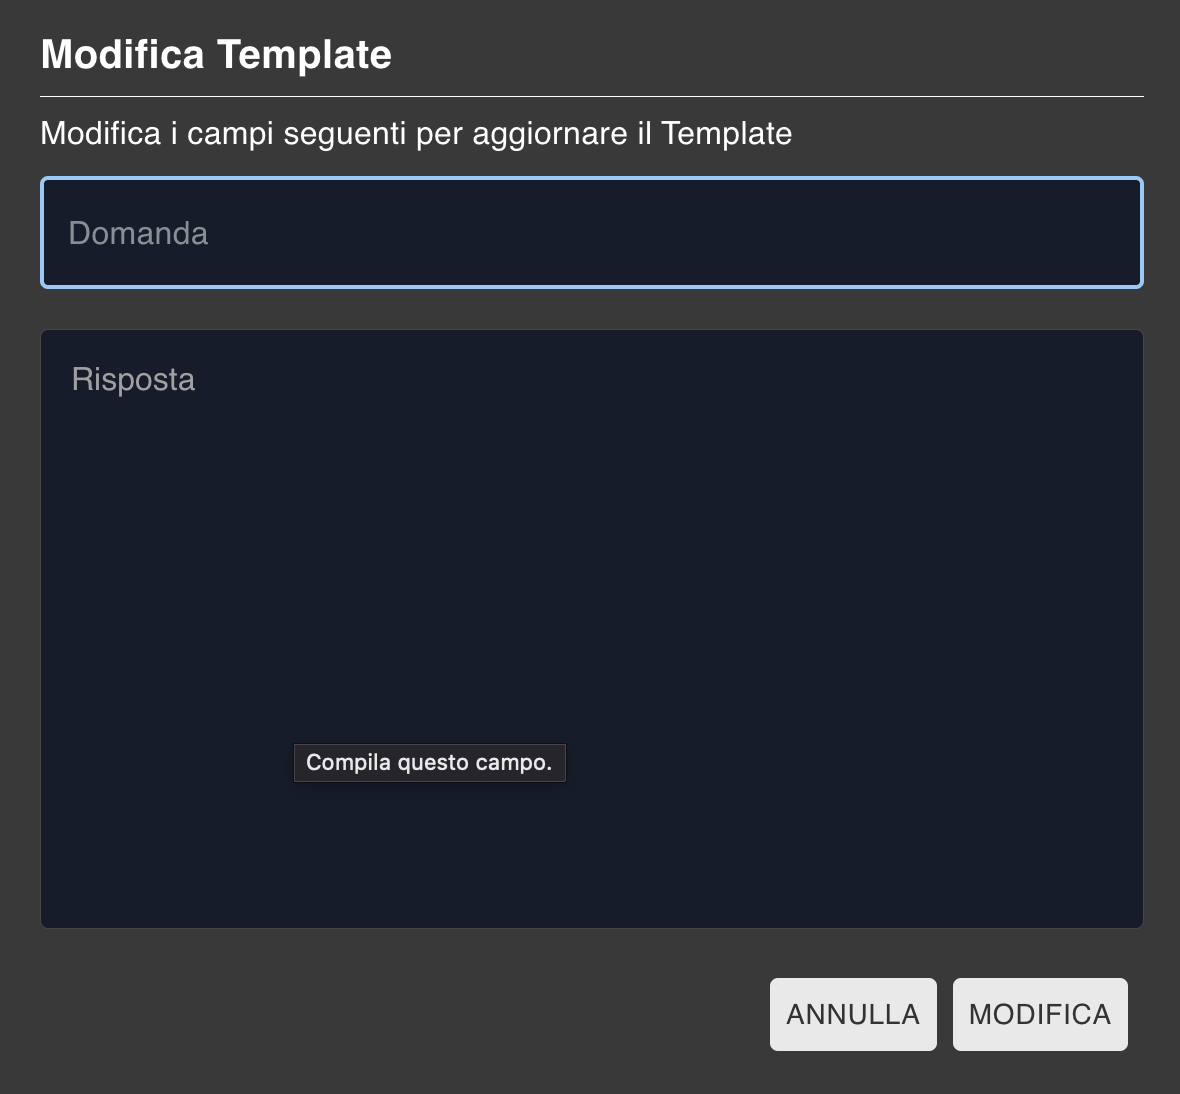
\includegraphics[width=0.7\textwidth]{./img/ModificaTemplate.png}
%         \caption{ModificaTemplate}
%     \end{subfigure}
%     \hspace{0.05\textwidth}
%     \begin{subfigure}{0.5\textwidth}
%         \centering
%         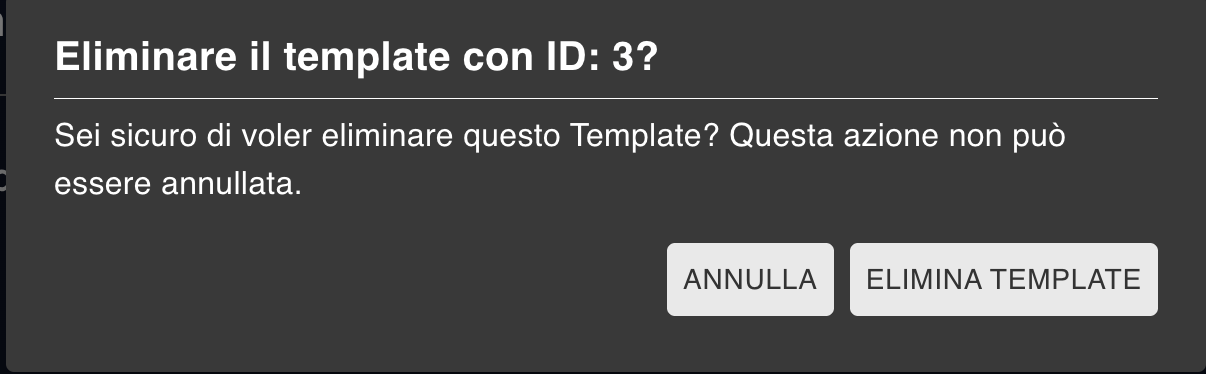
\includegraphics[width=\textwidth]{./img/EliminaTemplate.png}
%         \caption{Elimina Template}
%     \end{subfigure}
%     \caption{Modifica Template ed Elimina Template}
%     \label{fig:pop-up modifica ed elimina}
% \end{figure}

% \subsubsection{Assistenza Clienti}
% Cliccando dal menù laterale sulla voce "Assistenza clienti" (fig~\ref{fig:Assistenza1} pt.1) è possibile visualizzare tutte le richieste di assistenza che i vari utenti hanno inviato (fai riferimento alla sottosezione \textit{Pagina di Richiesta di Supporto} a pagina~\pageref{fig:Pagina di Assistenza}).
% Per ogni richiesta verranno visualizzate:
% \begin{itemize}
%     \item Lo stato della richiesta (fig~\ref{fig:Assistenza1} pt.2)
%     \begin{itemize}
%         \item \textbf{Rosso:} non gestita;
%         \item \textbf{Verde:} gestita;
%     \end{itemize}
%     \item email
%     \item data di invio da parte dell'utente %NOTA PER IL VERIFICATORE, forse qui vanno aggiunti dei punti nell'immagine come ho fatto io per le altre figure
%     \item oggetto della richiesta %Invito cortesemente a farlo basta modificare l'immagine, io ho usato gli strumenti presenti in antemprima su macOS quindi si può fare.
%     \item contenuto della richiesta %Perfavore Sto scrivendo il documento alle 2 di notte quindi verificatore lavora
%     \item pulsante di presa carico (fig~\ref{fig:Assistenza1} pt.3)
% \end{itemize}
% \begin{figure}[h!]
%     \centering
%     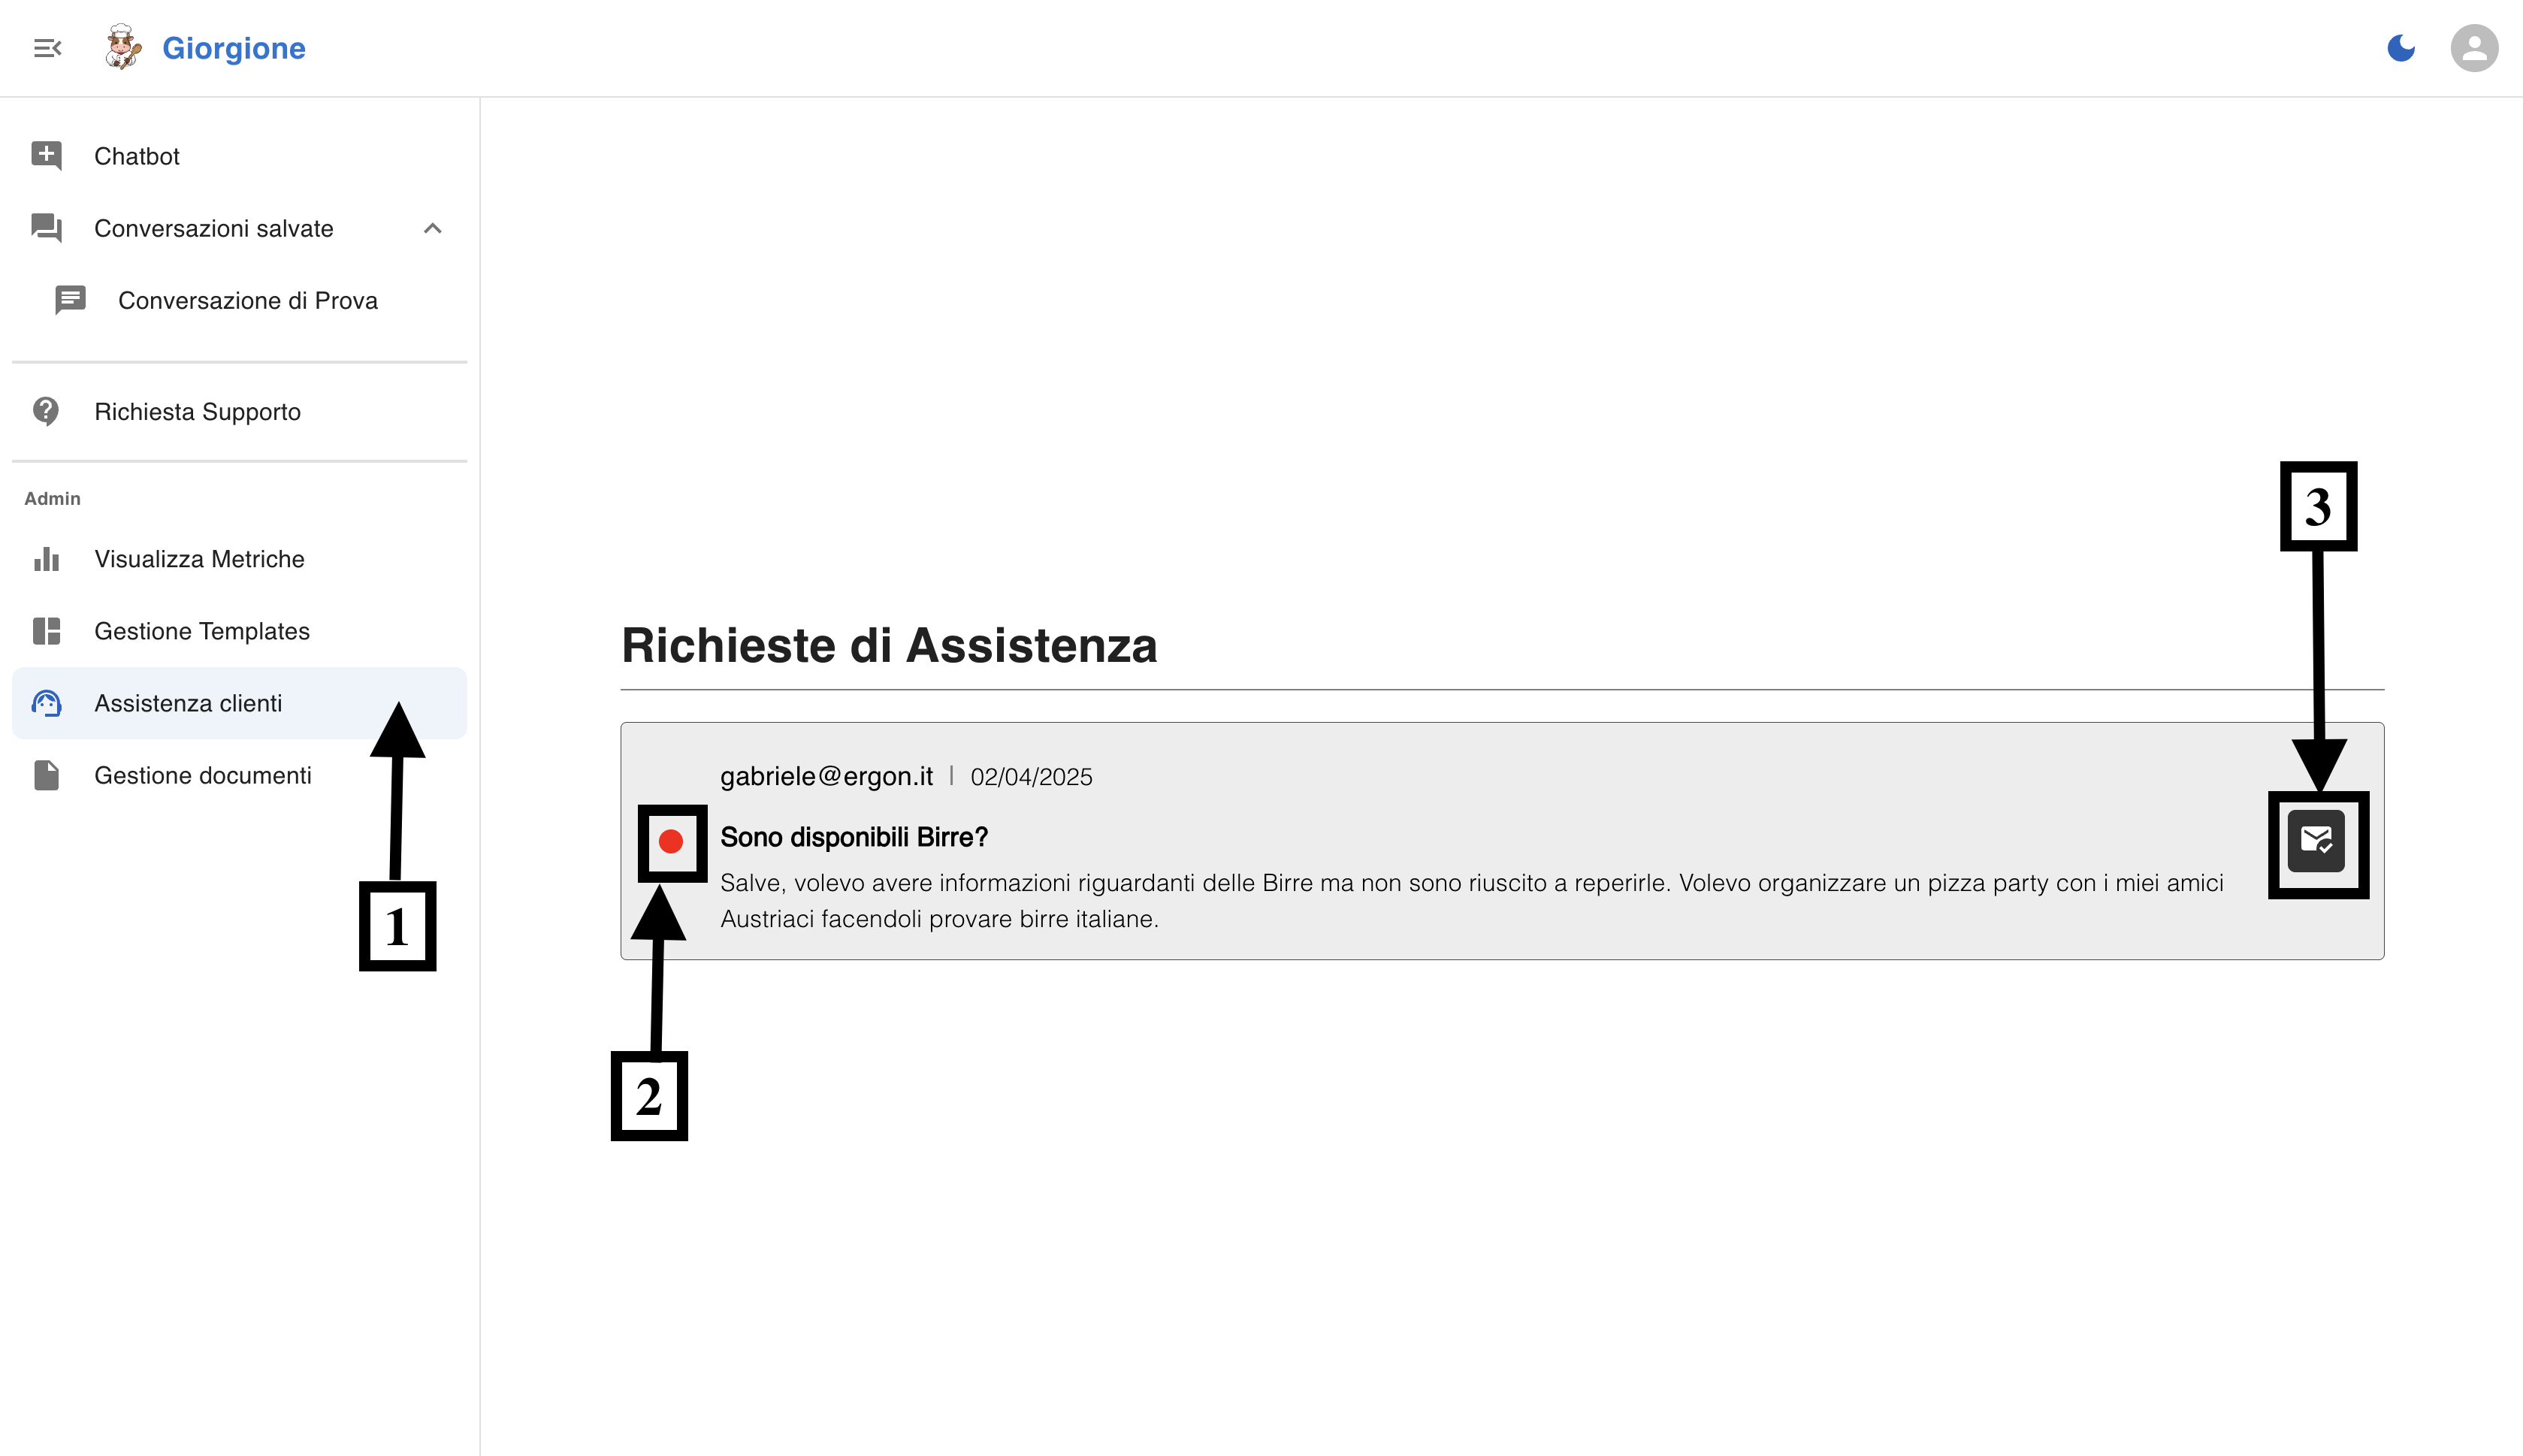
\includegraphics[width=\textwidth]{./img/Assistenza1.png}
%     \caption{Gestione Assistenza}
%     \label{fig:Assistenza1}
% \end{figure}
% Se la richiesta viene presa in carico cliccando il pulsante (fig~\ref{fig:Assistenza1} pt.3) il colore dello stato passerà da \textbf{Rosso} a \textbf{Verde}.
% \begin{figure}[h!]
%     \centering
%     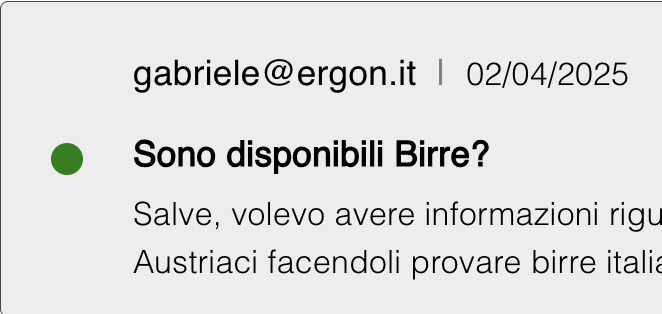
\includegraphics[width=0.5\textwidth]{./img/Assistenza2.png}
%     \caption{Colore Stato}
% \end{figure}

% \subsubsection{Gestione Documenti}
% Cliccando infine sulla pagina di gestione documenti ci troveremo davanti alla schermata mostrata in figura~\ref{fig:gestione1}, che permetterà di inserire file per addestrare il nostro assistente virtuale a rispondere a determinate domande.
% \begin{figure}[h!]
%     \centering
%     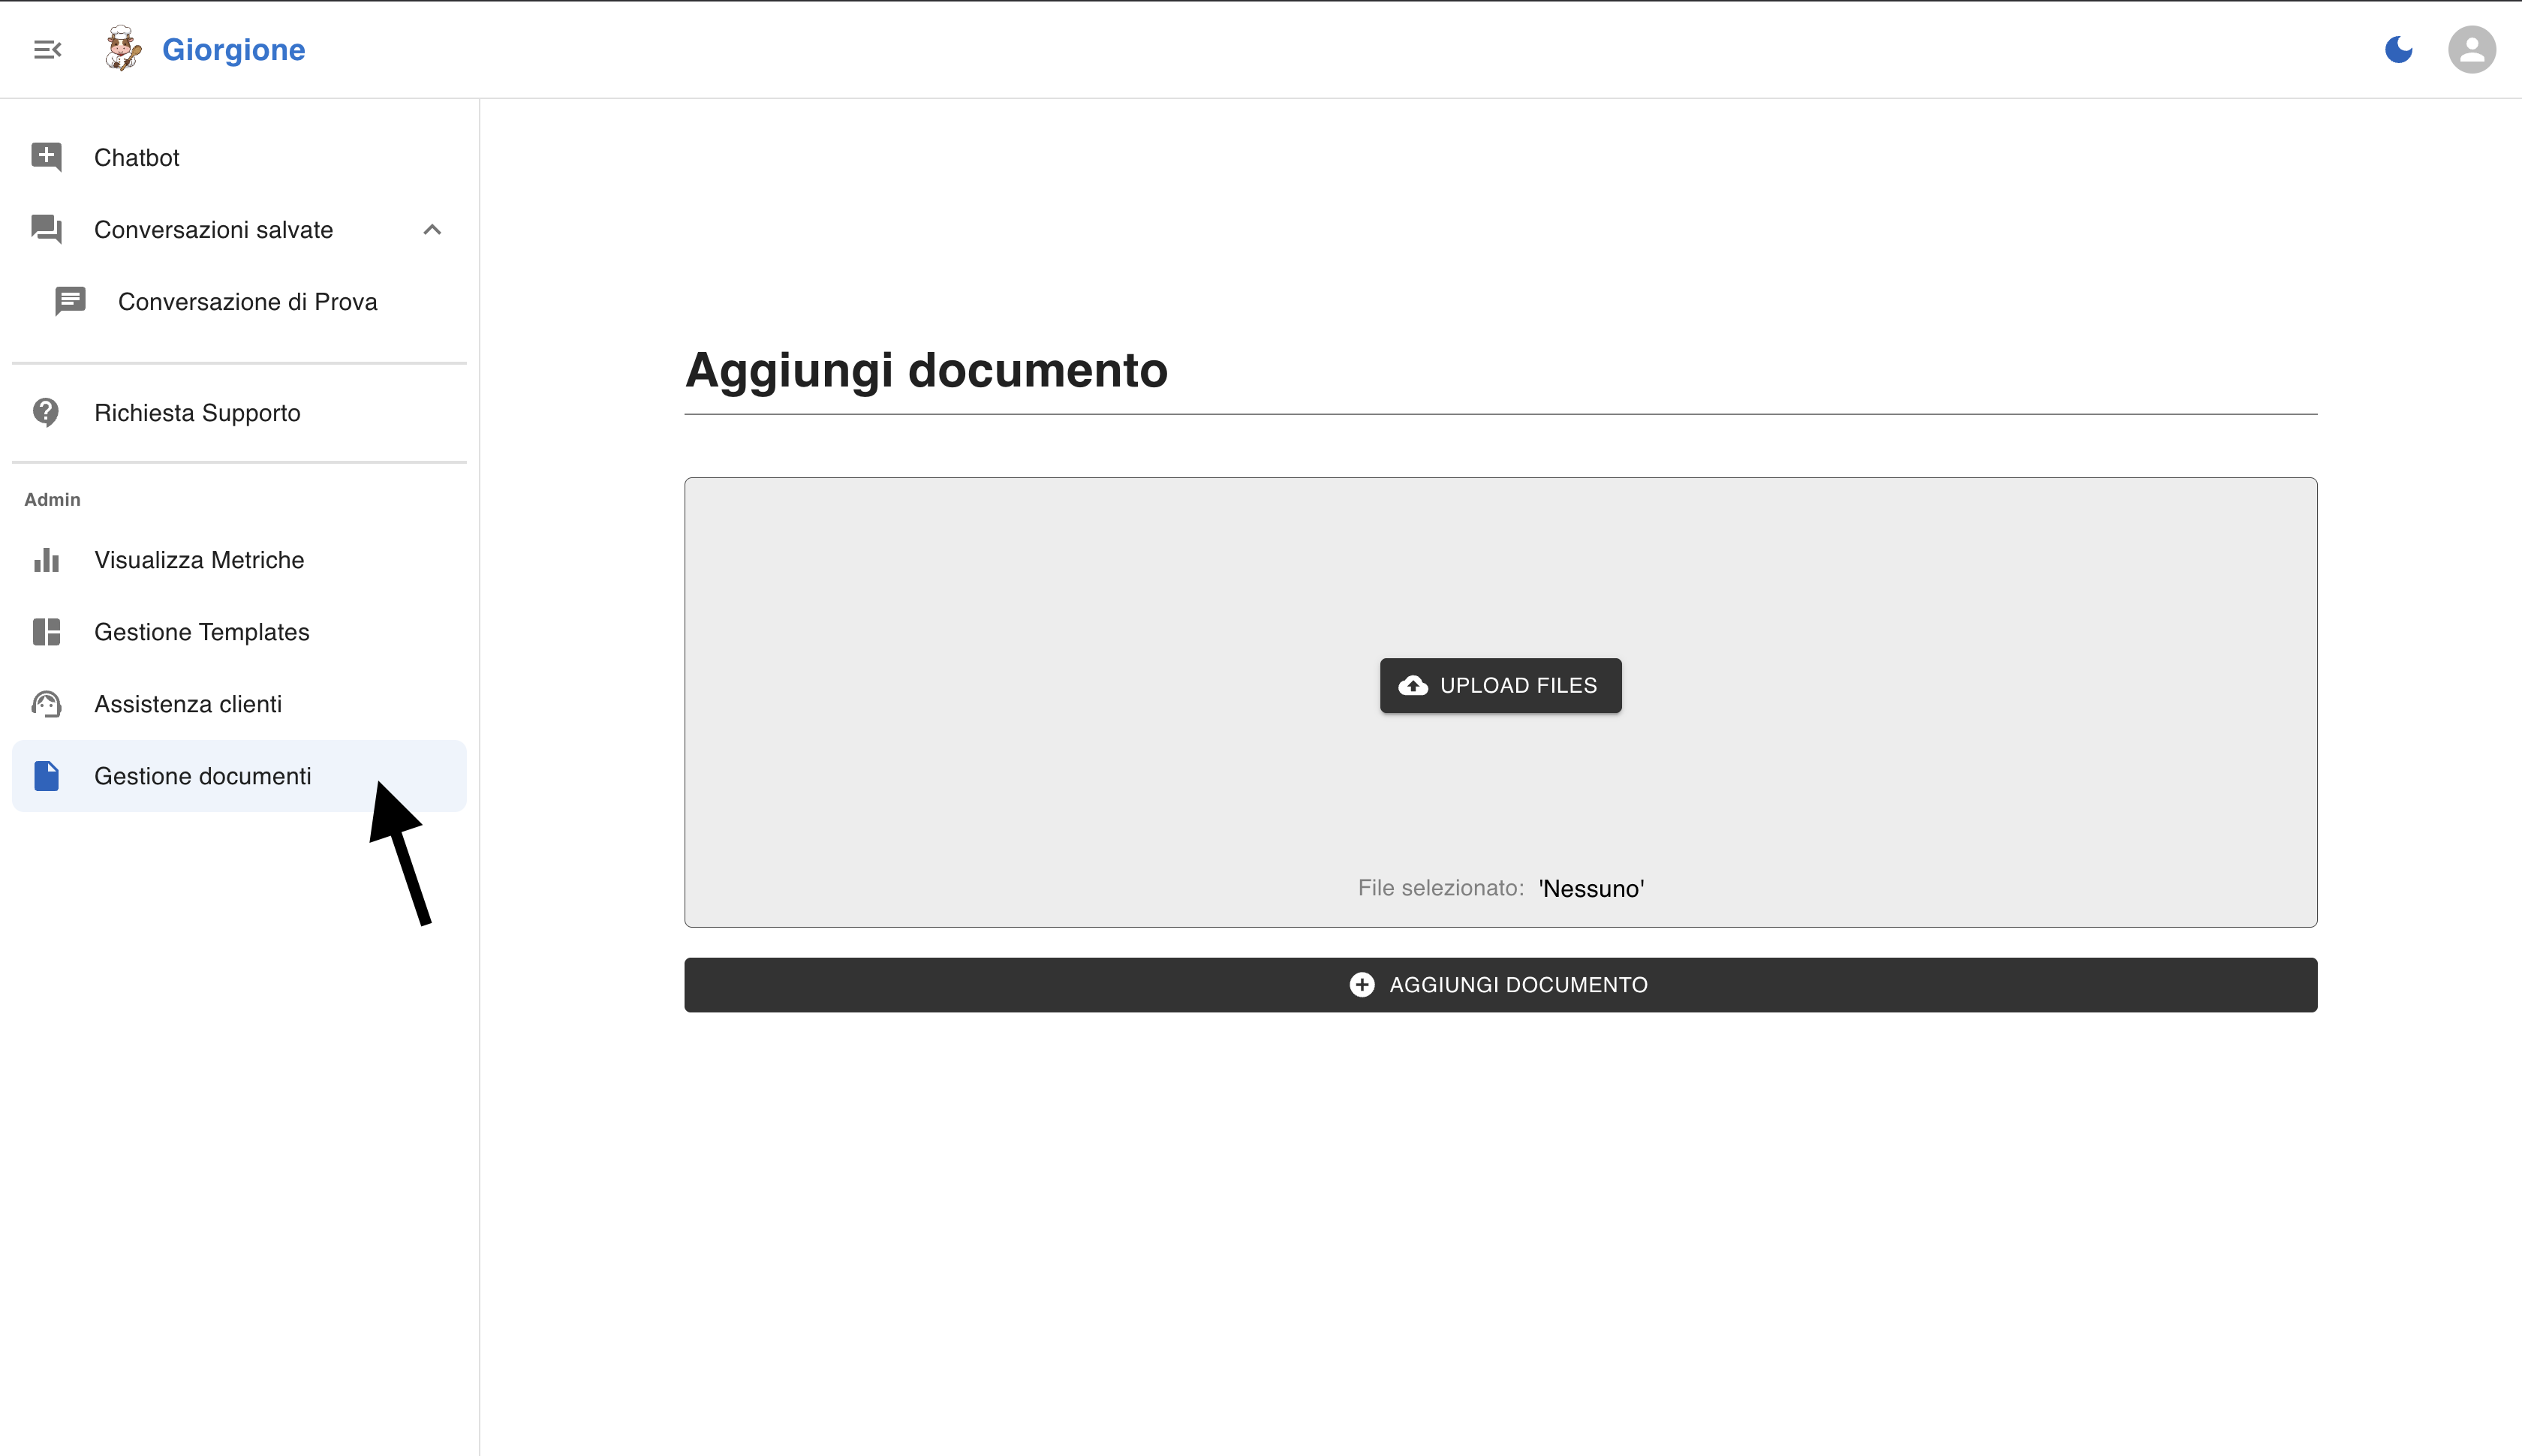
\includegraphics[width=0.8\textwidth]{./img/PaginaGestioneDocumenti1.png}
%     \caption{Pagina Gestione Documenti}
%     \label{fig:gestione1}
% \end{figure}

% Procediamo quindi ad illustrare come caricare i dati. Cominciamo quindi cliccando sul bottone "upload files" come indicato dalla freccia in figura~\ref{fig:gestione2}
% \begin{figure}[h!]
%     \centering
%     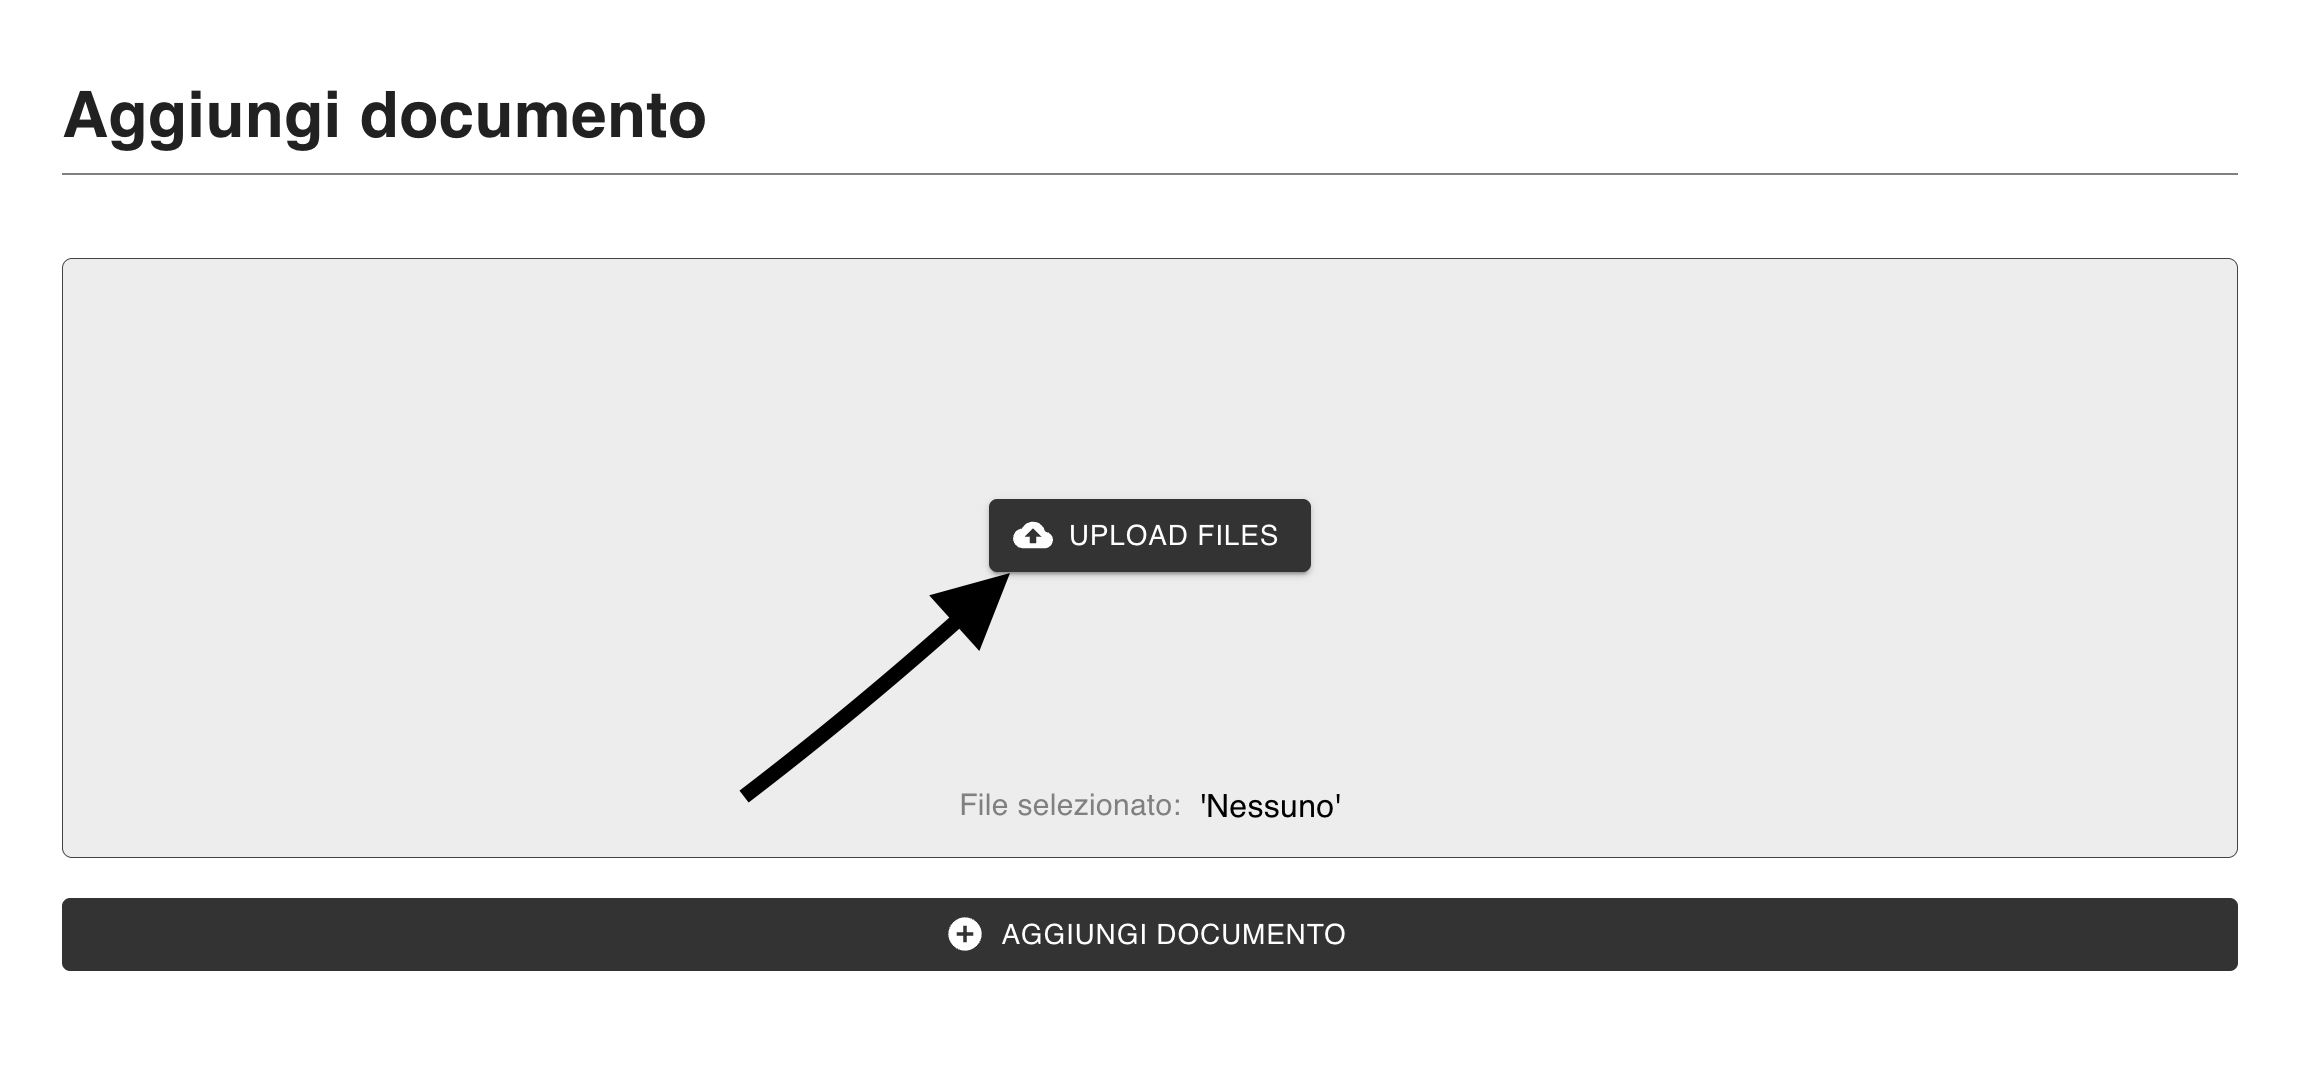
\includegraphics[width=0.6\textwidth]{./img/PaginaGestioneDocumenti2.png}
%     \caption{Upload Documenti}
%     \label{fig:gestione2}
% \end{figure}
% Questo aprirà una finestra di selezione file, il sistema accetta file di tipo \texttt{.pdf} o \texttt{.txt} .
 
% \begin{figure}[h!]
%     \centering
%     \begin{subfigure}{0.4\textwidth}
%         \centering
%         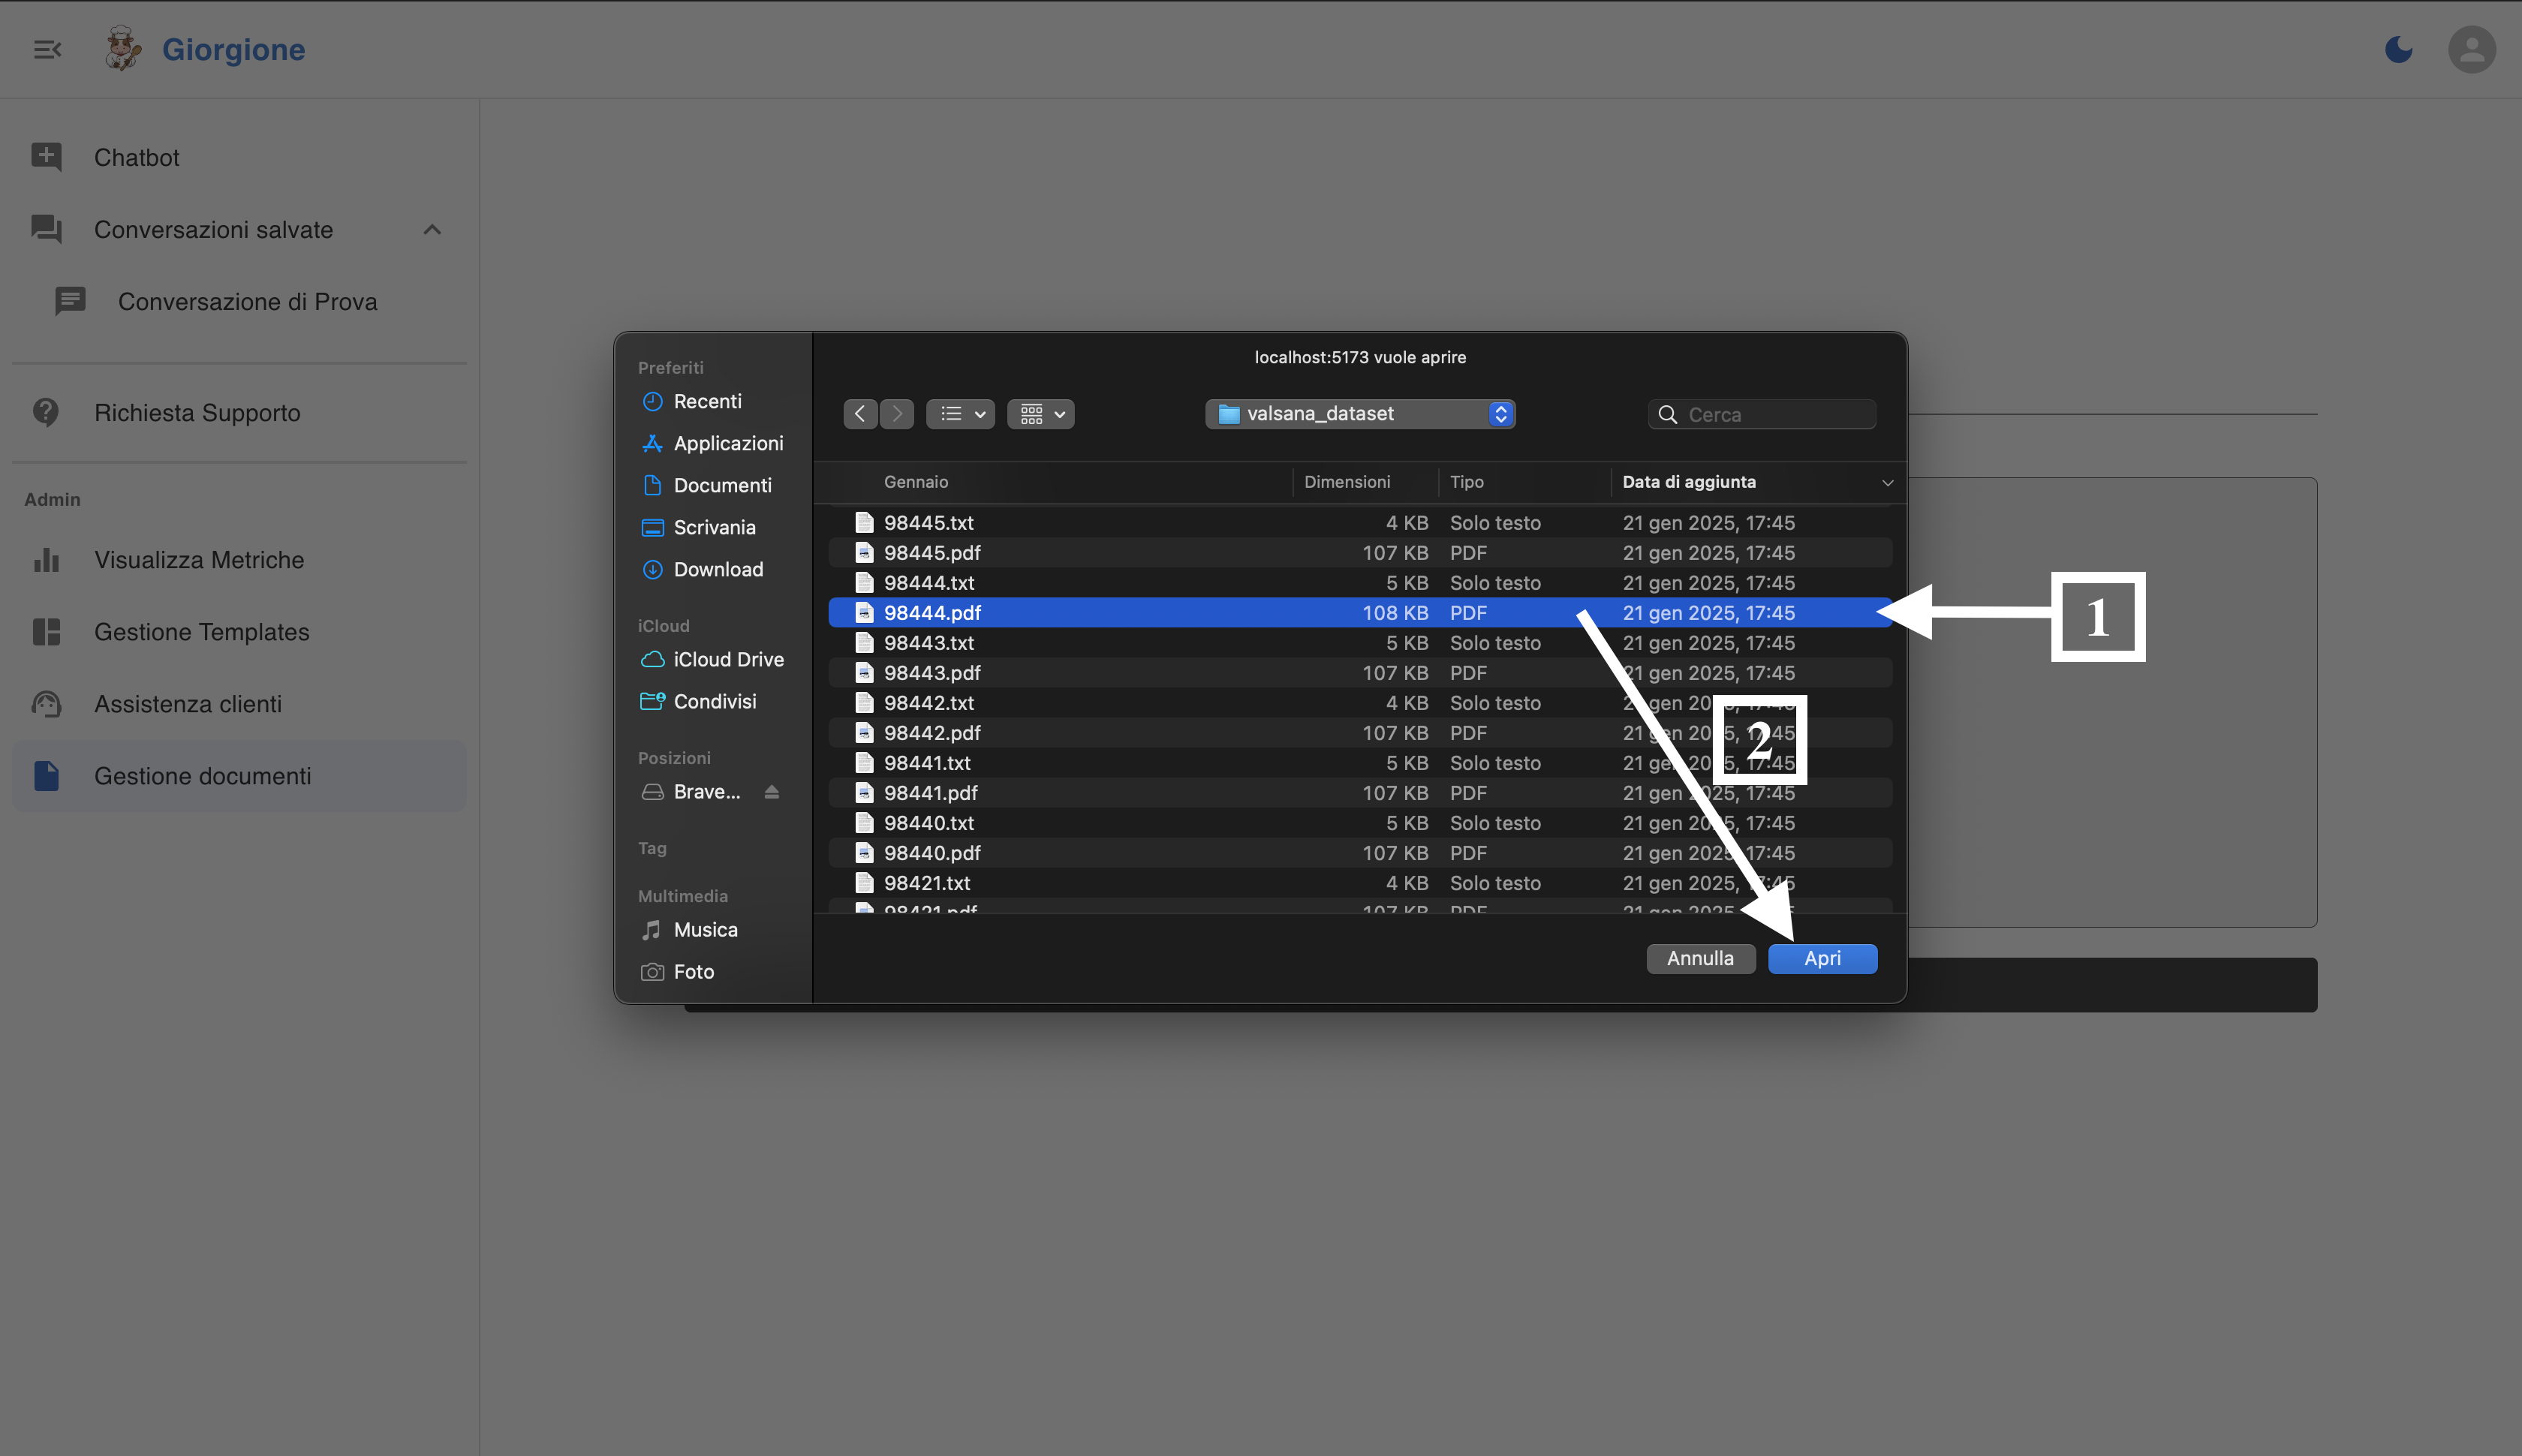
\includegraphics[width=\textwidth]{./img/PaginaGestioneDocumenti3.png}
%     \end{subfigure}
%     \hspace{0.05\textwidth}
%     \begin{subfigure}{0.4\textwidth}
%         \centering
%         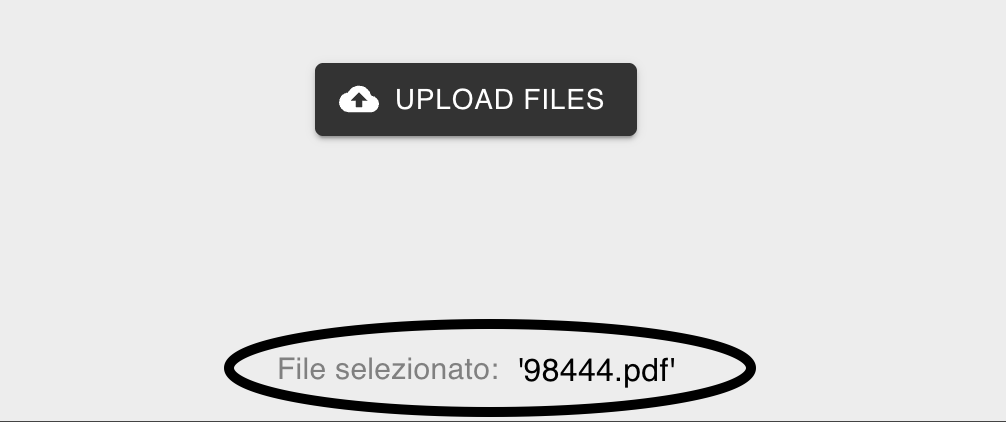
\includegraphics[width=\textwidth]{./img/GestioneDocumenti4.png}
%     \end{subfigure}
%     \caption{Inserimento file}
%     \label{fig:gestione3}
% \end{figure}
% Cliccando sul bottone aggiungi documento (fig~\ref{fig:gestione4} pt.1) l'admin verrà notificato dell'avvenuta riuscita (fig~\ref{fig:gestione4} pt.2) dell'operazione o del suo fallimento.
% \begin{figure}[h!]
%     \centering
%     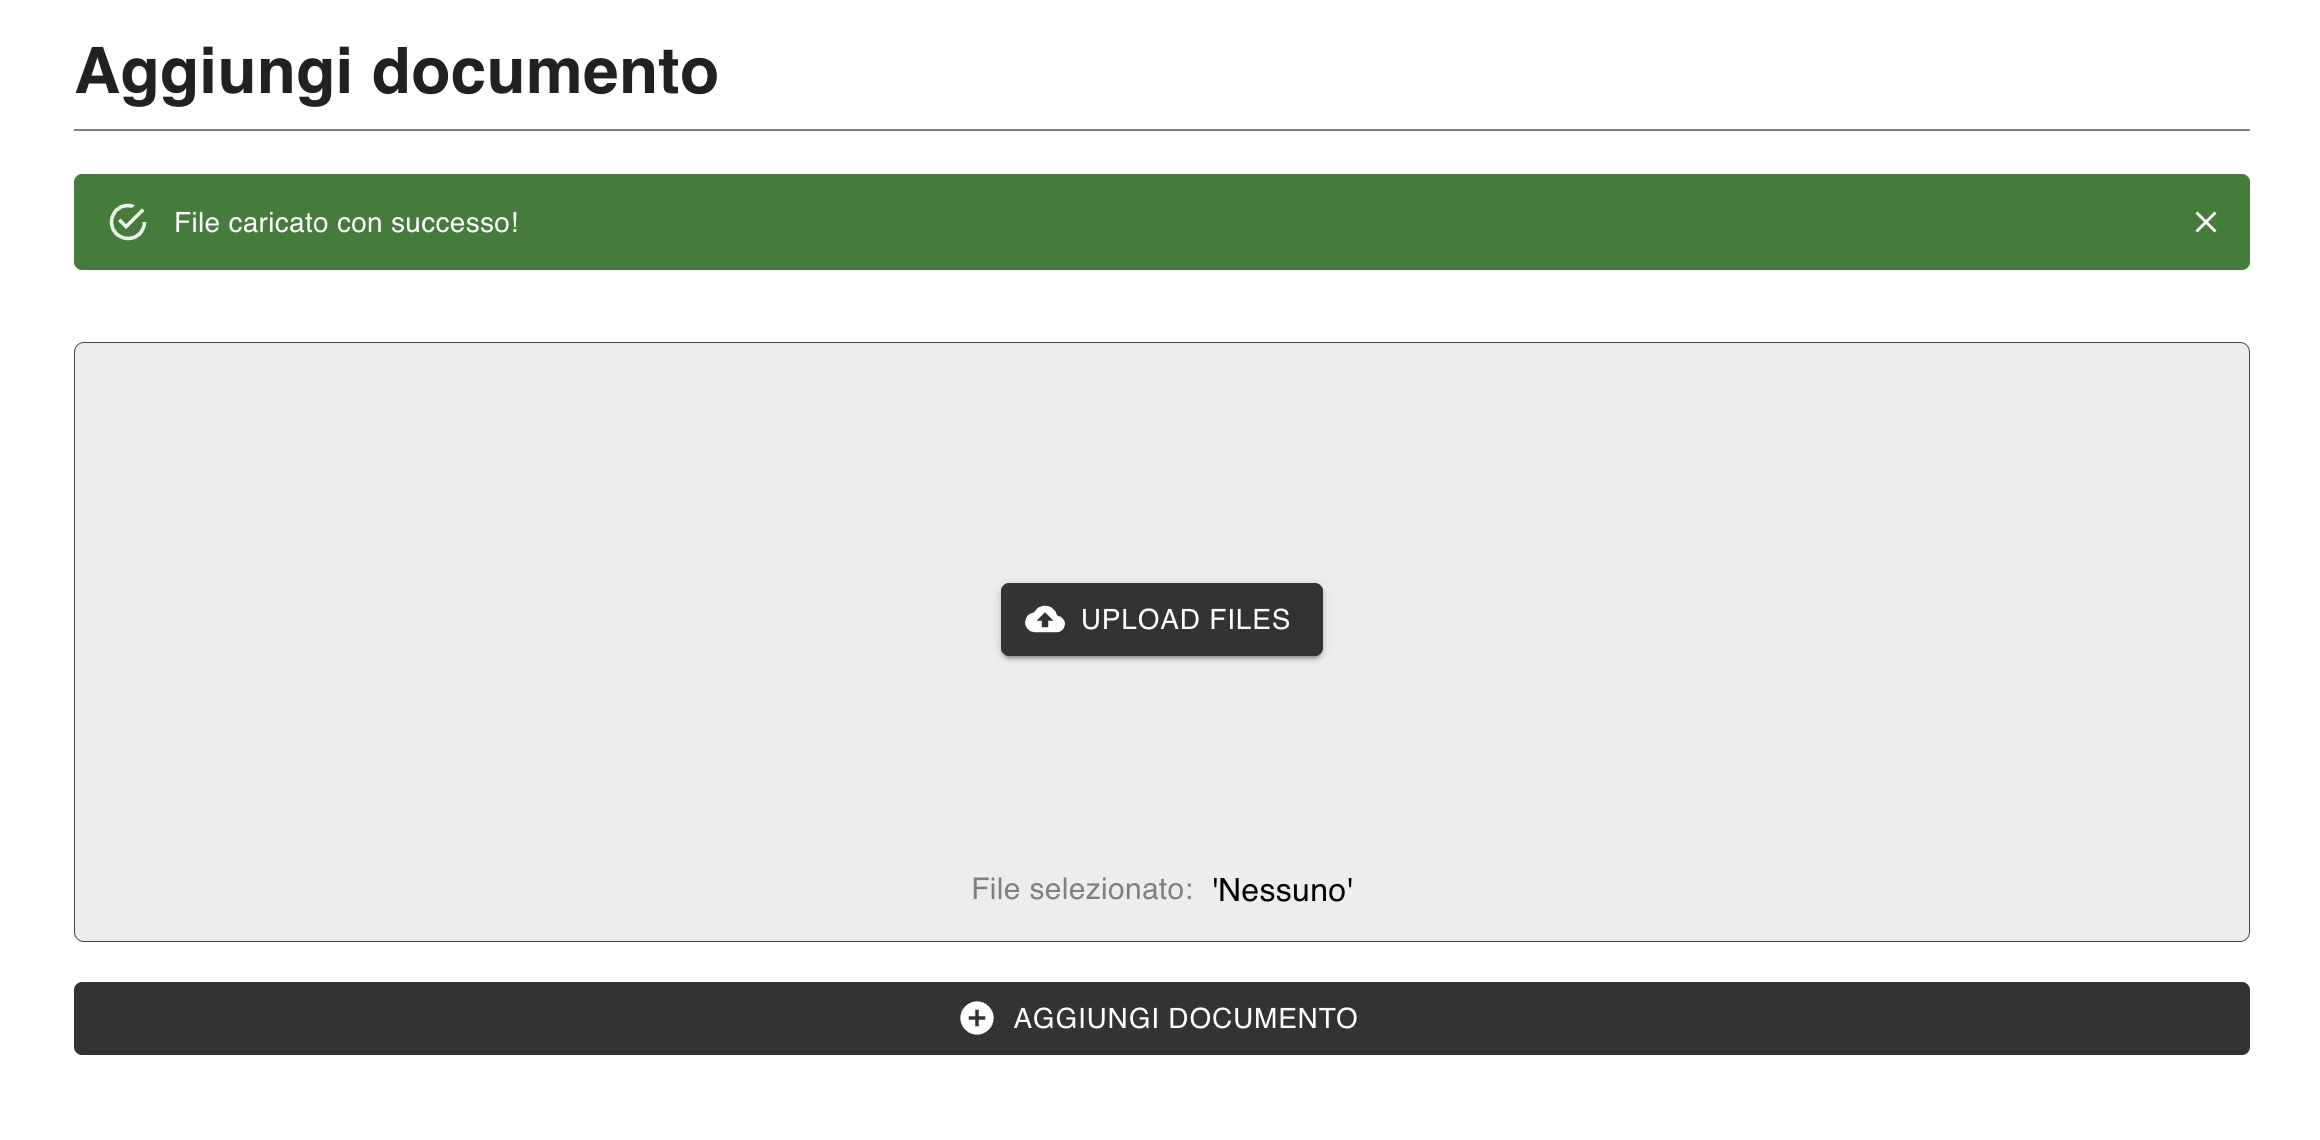
\includegraphics[width=0.8\textwidth]{./img/GestioneDocumenti5.png}
%     \caption{Upload Documenti con successo}
%     \label{fig:gestione4}
% \end{figure}

\section{Istruzioni all'uso}

\subsection{Pagine User}

\subsubsection{Landing page}
All'avvio del prodotto verrà visualizzata la landing page, che presenta il logo dell'assistente virtuale e un messaggio di benvenuto. In questa fase, l'utente può scegliere di accedere al sistema.
\begin{center}
    \includegraphics[width=\textwidth]{./img/landingPage.png}
    \captionof{figure}{Schermata della landing page}
\end{center}

\subsubsection{Pagina di Accesso}
Cliccando sul bottone blu si passerà alla pagina di accesso, dove l'utente dovrà inserire le proprie credenziali (\textit{username} e \textit{password}) per autenticarsi.
\begin{center}
    \includegraphics[width=\textwidth]{./img/paginaAccesso.png}
    \captionof{figure}{Schermata della pagina di accesso}
\end{center}

\subsubsection{Pagina di Registrazione}
Nel caso in cui non si possieda un account, è possibile registrarsi dalla pagina di registrazione cliccando sul link presente nella pagina di autenticazione. L'utente dovrà inserire i campi obbligatori \{\textit{username; password; email; nome; cognome}\} e, facoltativamente, il numero di telefono.
\begin{center}
    \includegraphics[width=\textwidth]{./img/paginaRegistrazione.png}
    \captionof{figure}{Schermata della pagina di registrazione}
\end{center}

\subsubsection{Schermata iniziale}
Una volta effettuato l'accesso, l'utente viene accolto da una schermata composta da una navbar superiore, una laterale e il contenuto principale. È possibile iniziare una conversazione inserendo il titolo e cliccando su "Inizia la conversazione".
\begin{center}
    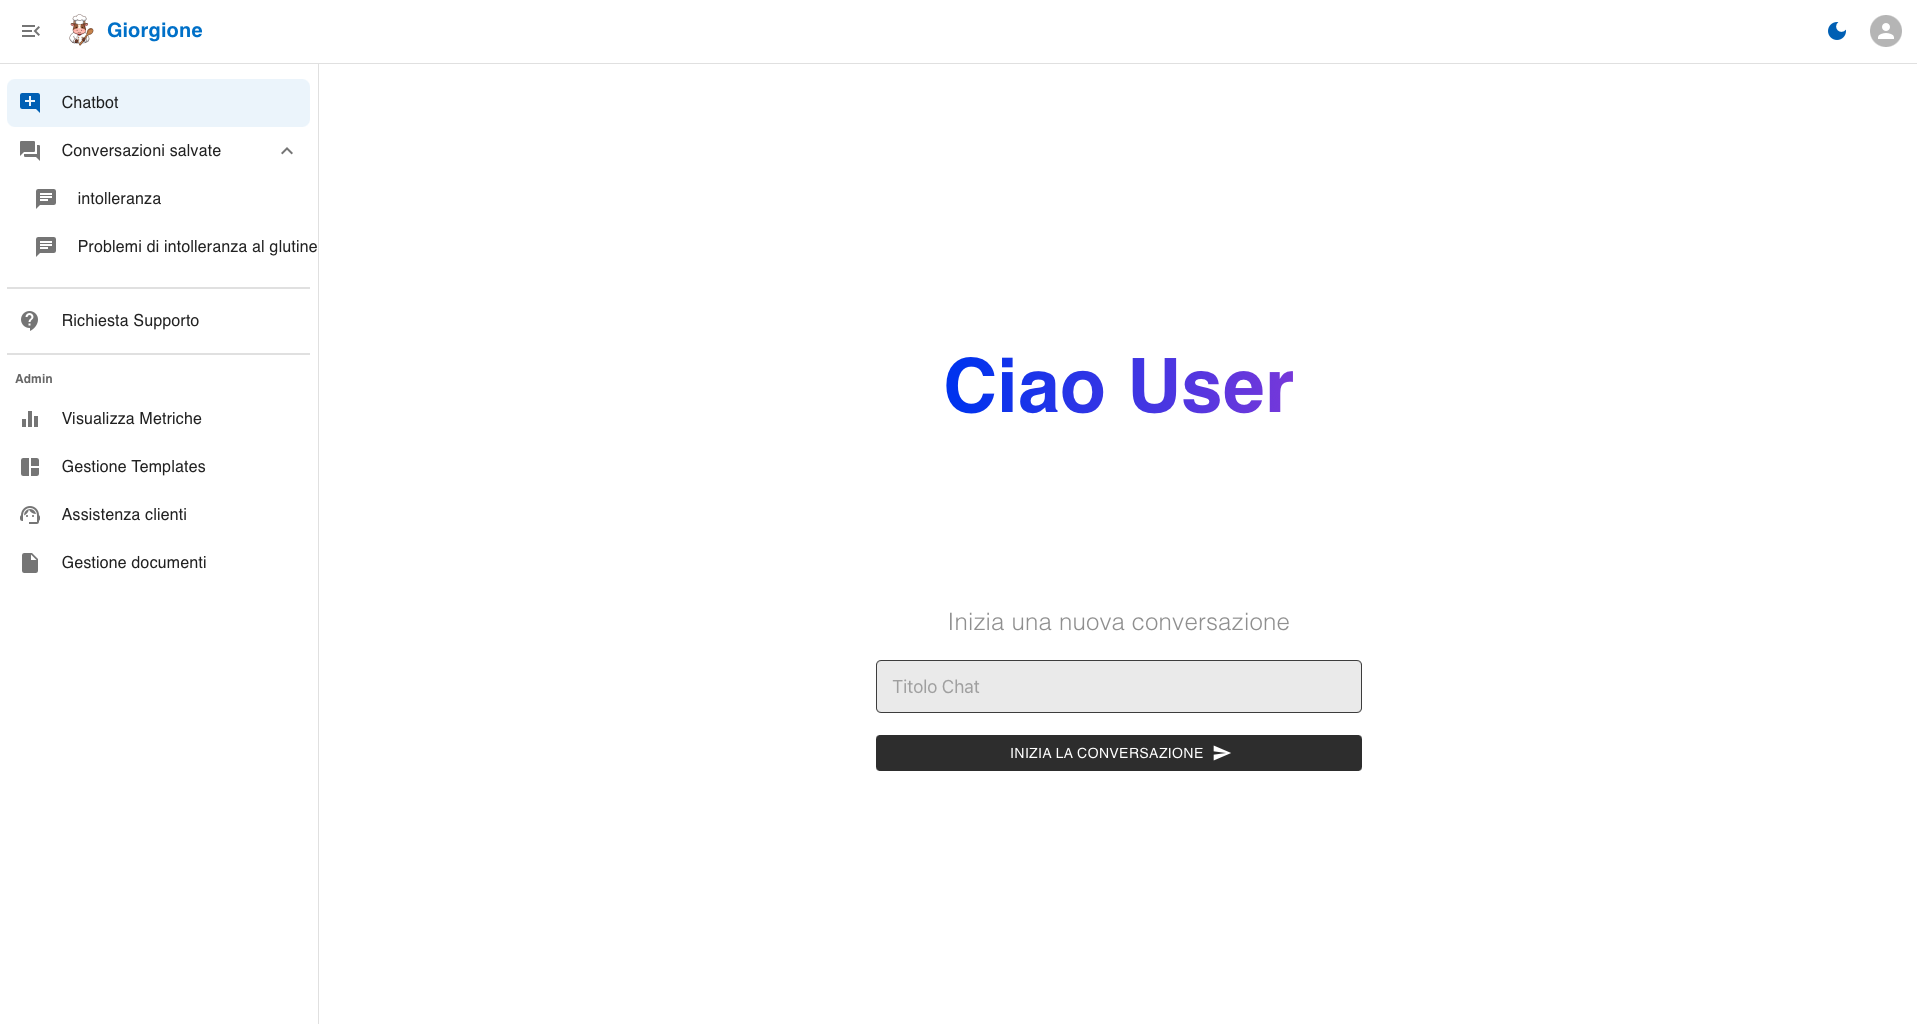
\includegraphics[width=\textwidth]{./img/paginaIniziale.png}
    \captionof{figure}{Schermata iniziale}
\end{center}

\subsubsection{Schermata di conversazione}
Dalla schermata iniziale è possibile accedere alle conversazioni salvate tramite il menù laterale (aperto tramite menù hamburger, se chiuso).
\begin{center}
    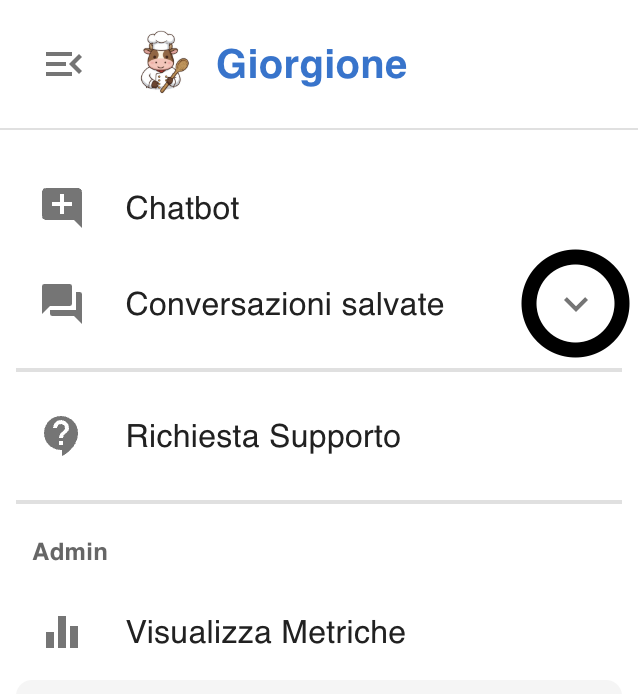
\includegraphics[width=0.3\textwidth]{./img/laterale1.png}
    \hspace{0.05\textwidth}
    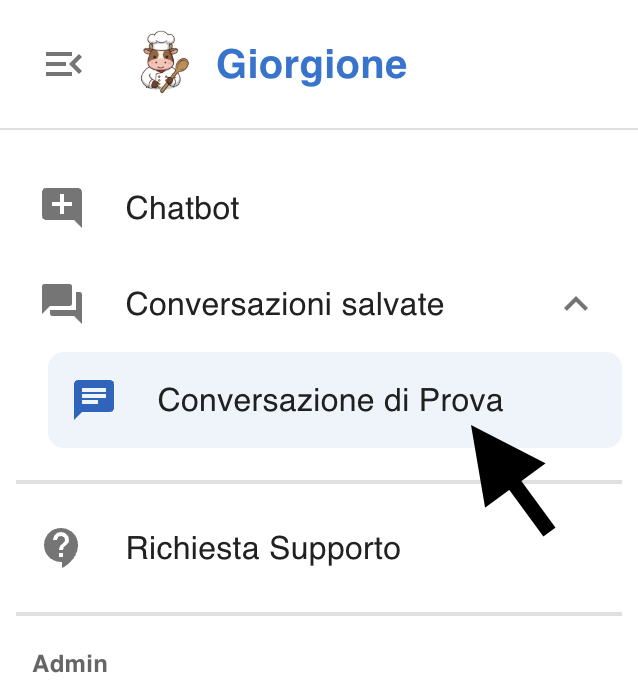
\includegraphics[width=0.3\textwidth]{./img/laterale2.png}
    \captionof{figure}{Menù laterale}
\end{center}

\begin{center}
    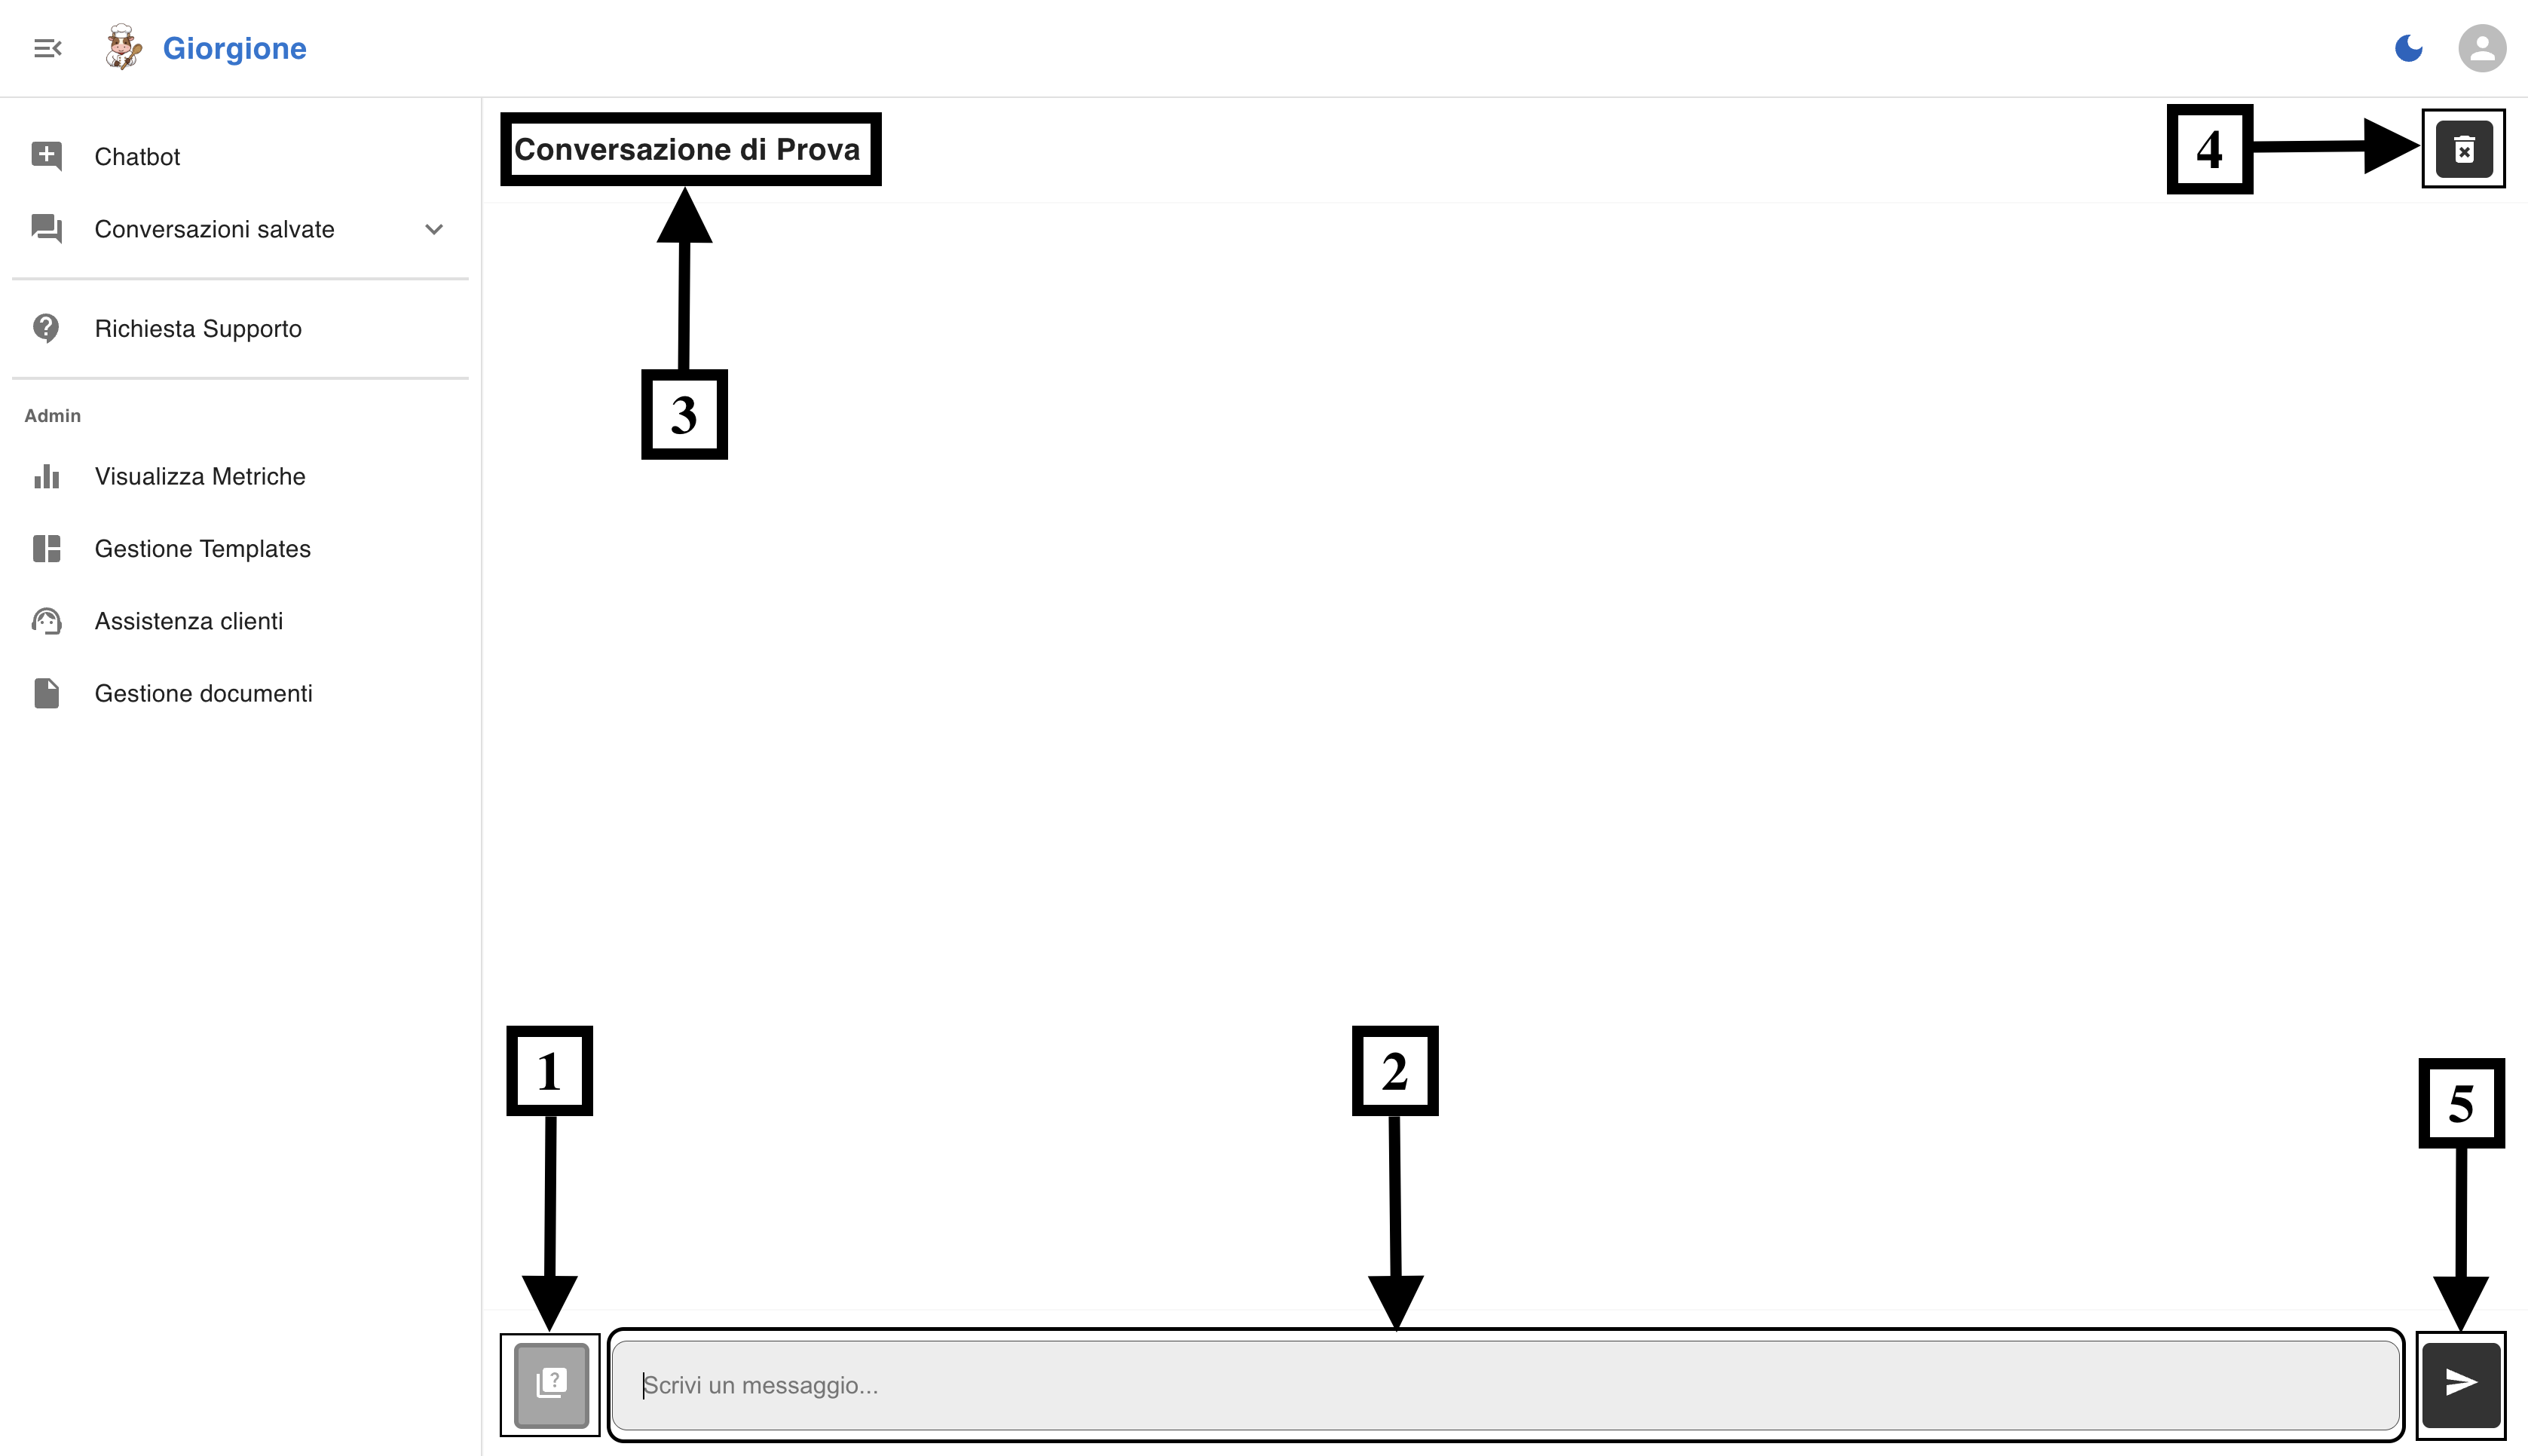
\includegraphics[width=\textwidth]{./img/SchermataChat1.png}
    \captionof{figure}{Schermata della chat}
    \label{fig:schermata-chat}
\end{center}

Facendo riferimento alla figura~\ref{fig:schermata-chat}:

\begin{itemize}
    \item (1) Bottone per selezionare domande templetizzate.
    \item (2) Casella di testo per scrivere il messaggio.
    \item (3) Nome della conversazione.
    \item (4) Bottone per eliminare la chat, mostra un pop-up di conferma.
    \item (5) Pulsante invio, attivo solo se la casella contiene testo. Si può usare anche il tasto "invio" della tastiera.
\end{itemize}

\begin{center}
    \begin{tikzpicture}
        \node[anchor=east,inner sep=0] (img1) at (0,0) {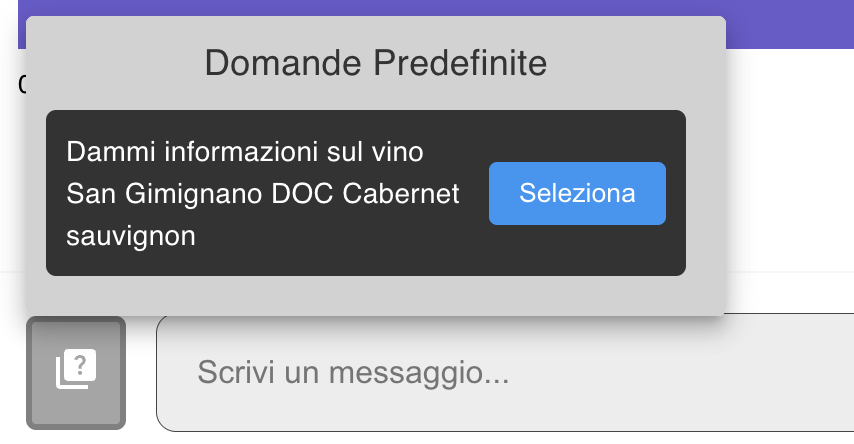
\includegraphics[width=0.4\textwidth]{img/SelettoreTemplate1.png}};
        \node[anchor=west,inner sep=0] (img2) at (2,0) {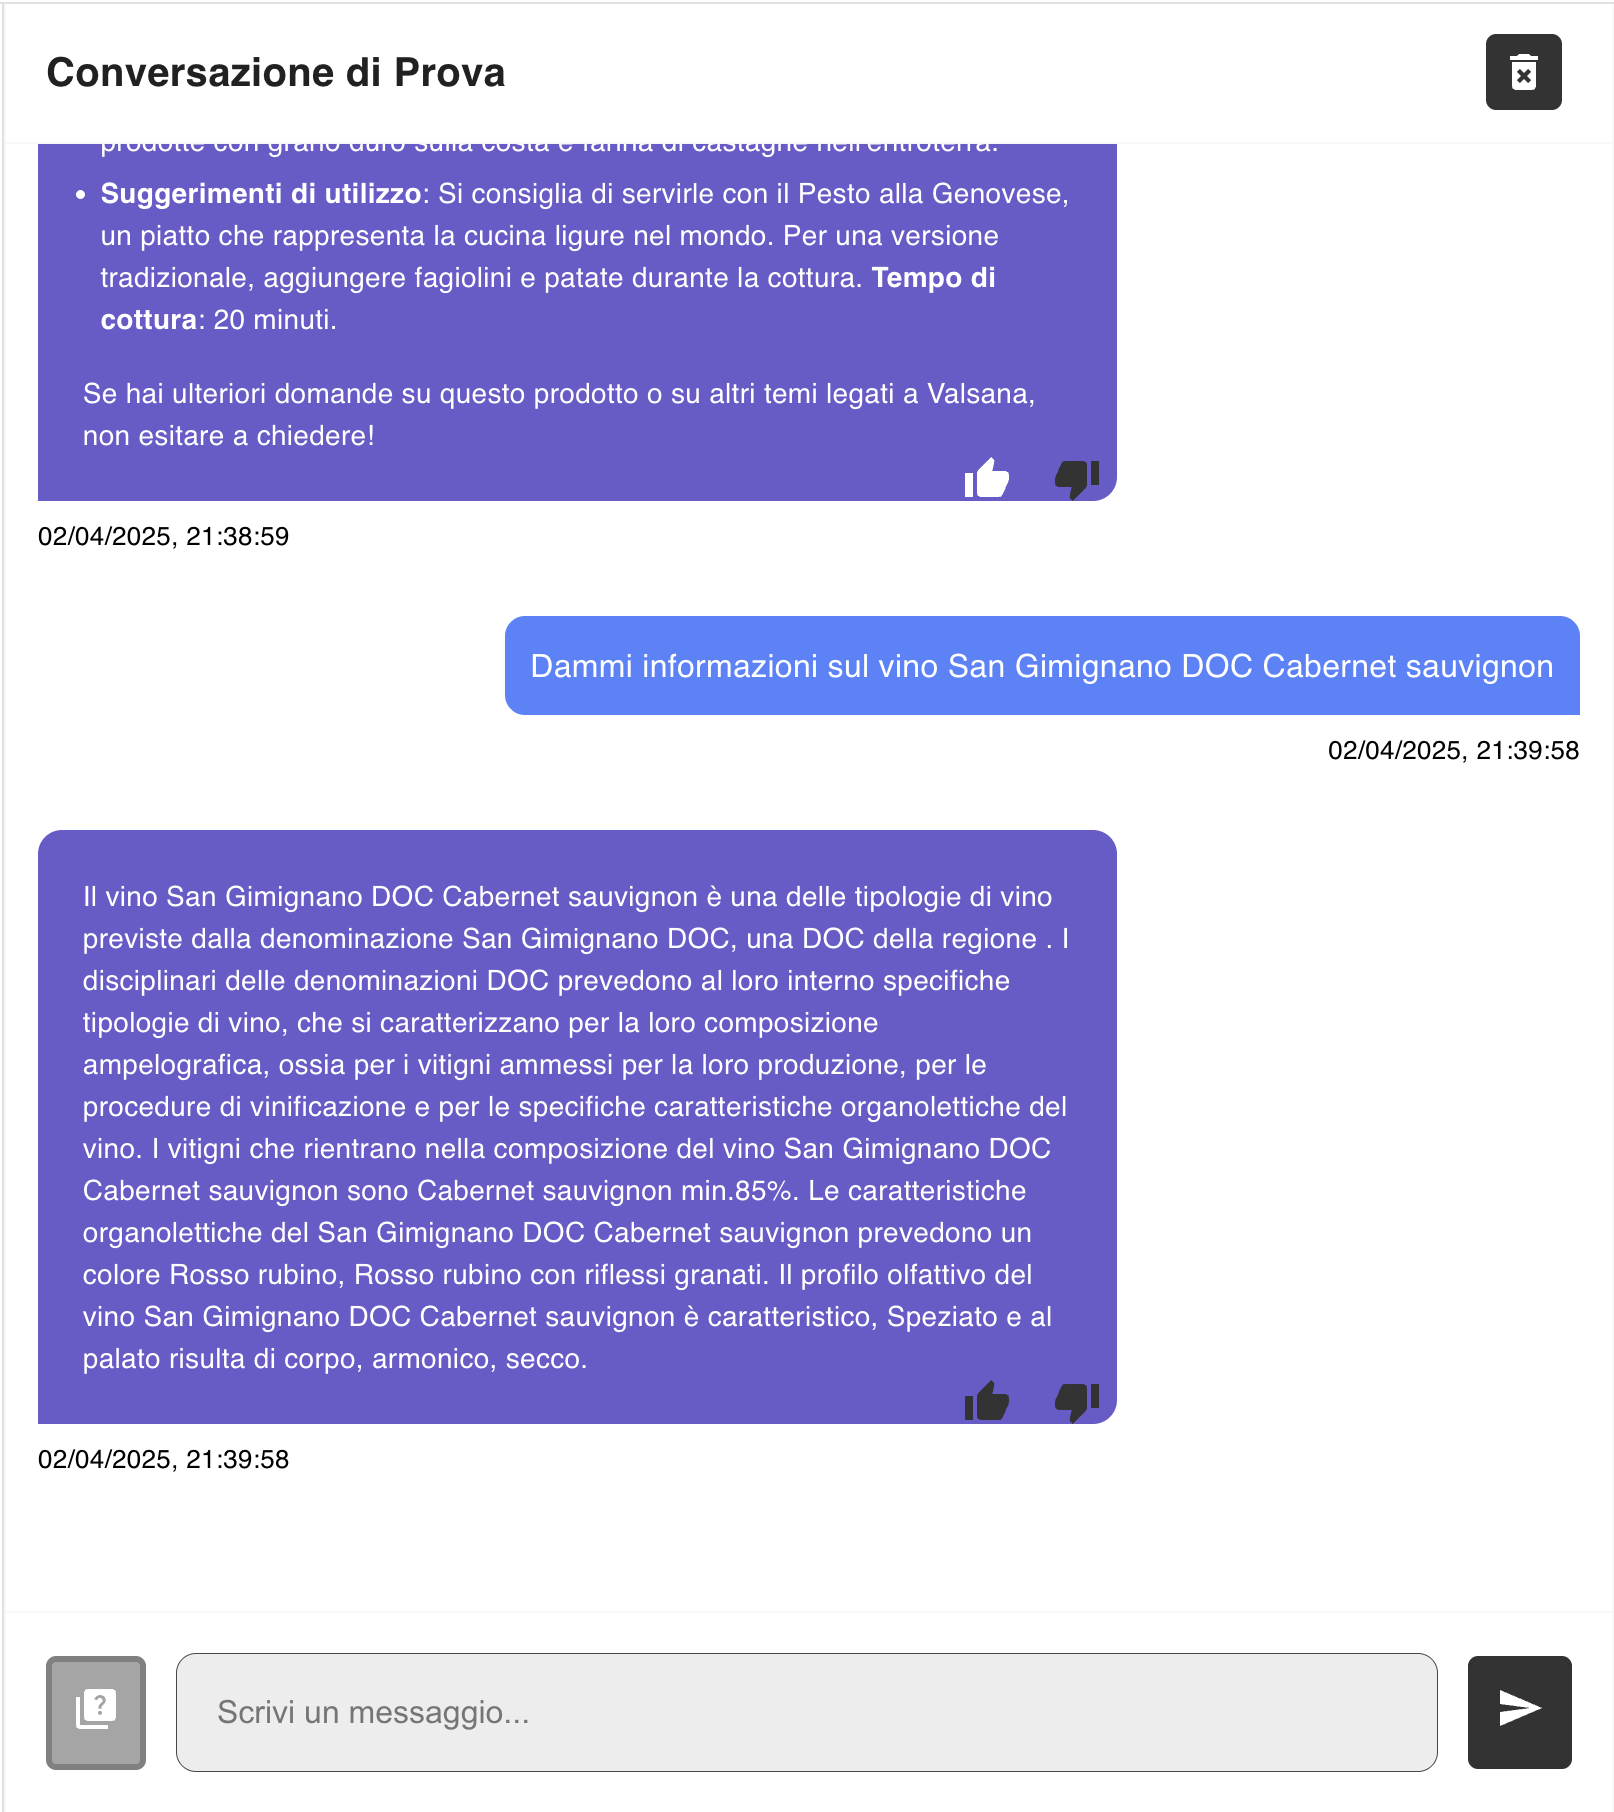
\includegraphics[width=0.4\textwidth]{img/SelettoreTemplate2.png}};
        \draw[->, thick] (img1.east) -- (img2.west);
    \end{tikzpicture}
    \captionof{figure}{Selezione domanda templetizzata}
    \label{fig:domanda templetizzata}
\end{center}

\begin{center}
    
\includegraphics[width=0.5\textwidth]{./img/eliminaChat.png}
    \captionof{figure}{Conferma eliminazione chat}
    \label{fig:elimina-chat}
\end{center}

\begin{center}
    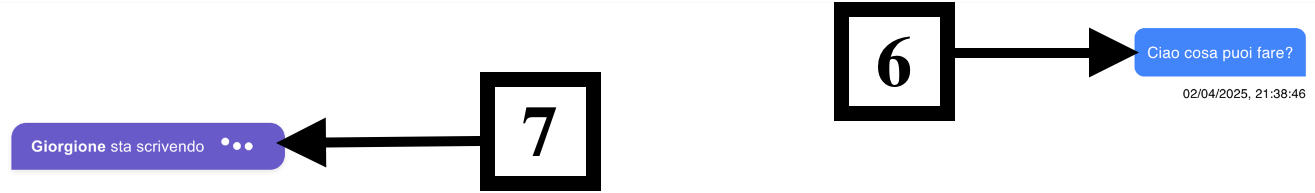
\includegraphics[width=\textwidth]{./img/SchermataChat2.png}
    \captionof{figure}{Elaborazione del messaggio}
    \label{fig:Elaborazione}
\end{center}

\begin{center}
    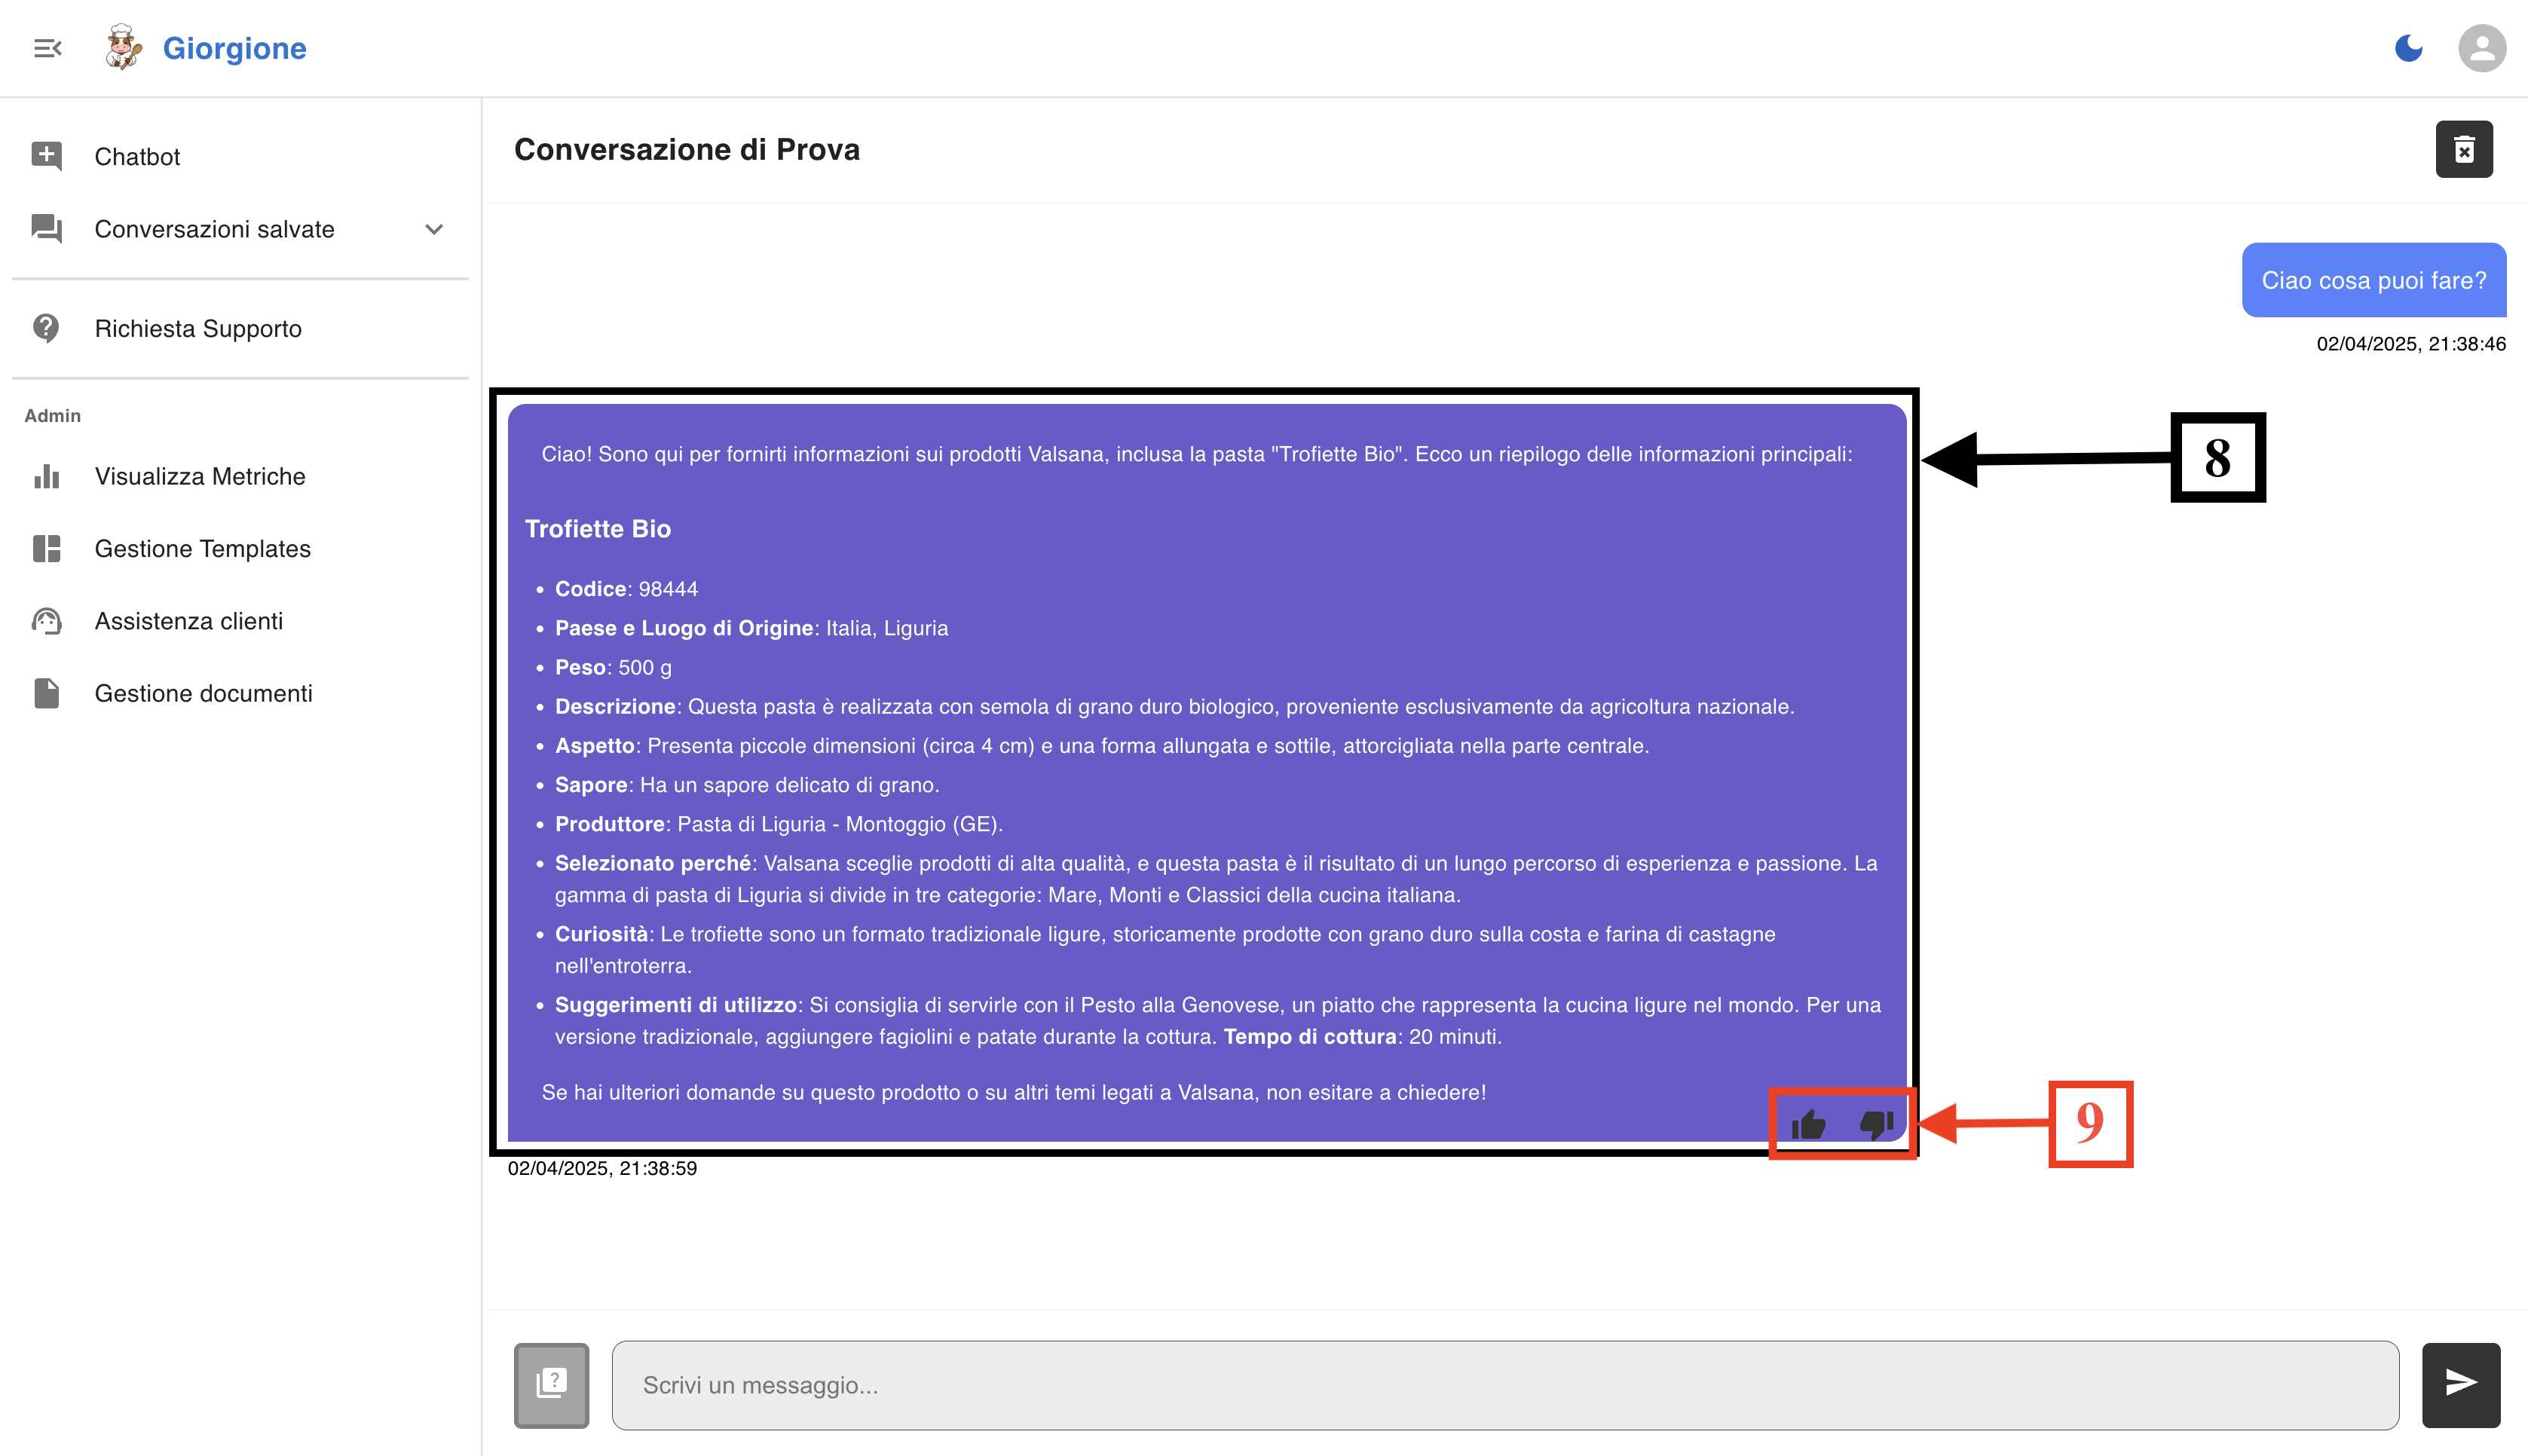
\includegraphics[width=\textwidth]{./img/SchermataChat3.png}
    \captionof{figure}{Visualizzazione risposta e feedback}
    \label{fig:Visualizzazione Risposta}
\end{center}

\begin{center}
    
\includegraphics[width=0.2\textwidth]{./img/like.png}
    \hspace{0.05\textwidth}
    
\includegraphics[width=0.2\textwidth]{./img/dislike.png}
    \captionof{figure}{Feedback utente: like o dislike}
    \label{fig:likedislike}
\end{center}

\subsubsection{Pagina di Richiesta di Supporto}
Dal menù laterale si accede alla pagina "Richiesta Supporto". L’utente può inviare una segnalazione inserendo oggetto, descrizione e inviando tramite l’apposito bottone.
\begin{center}
    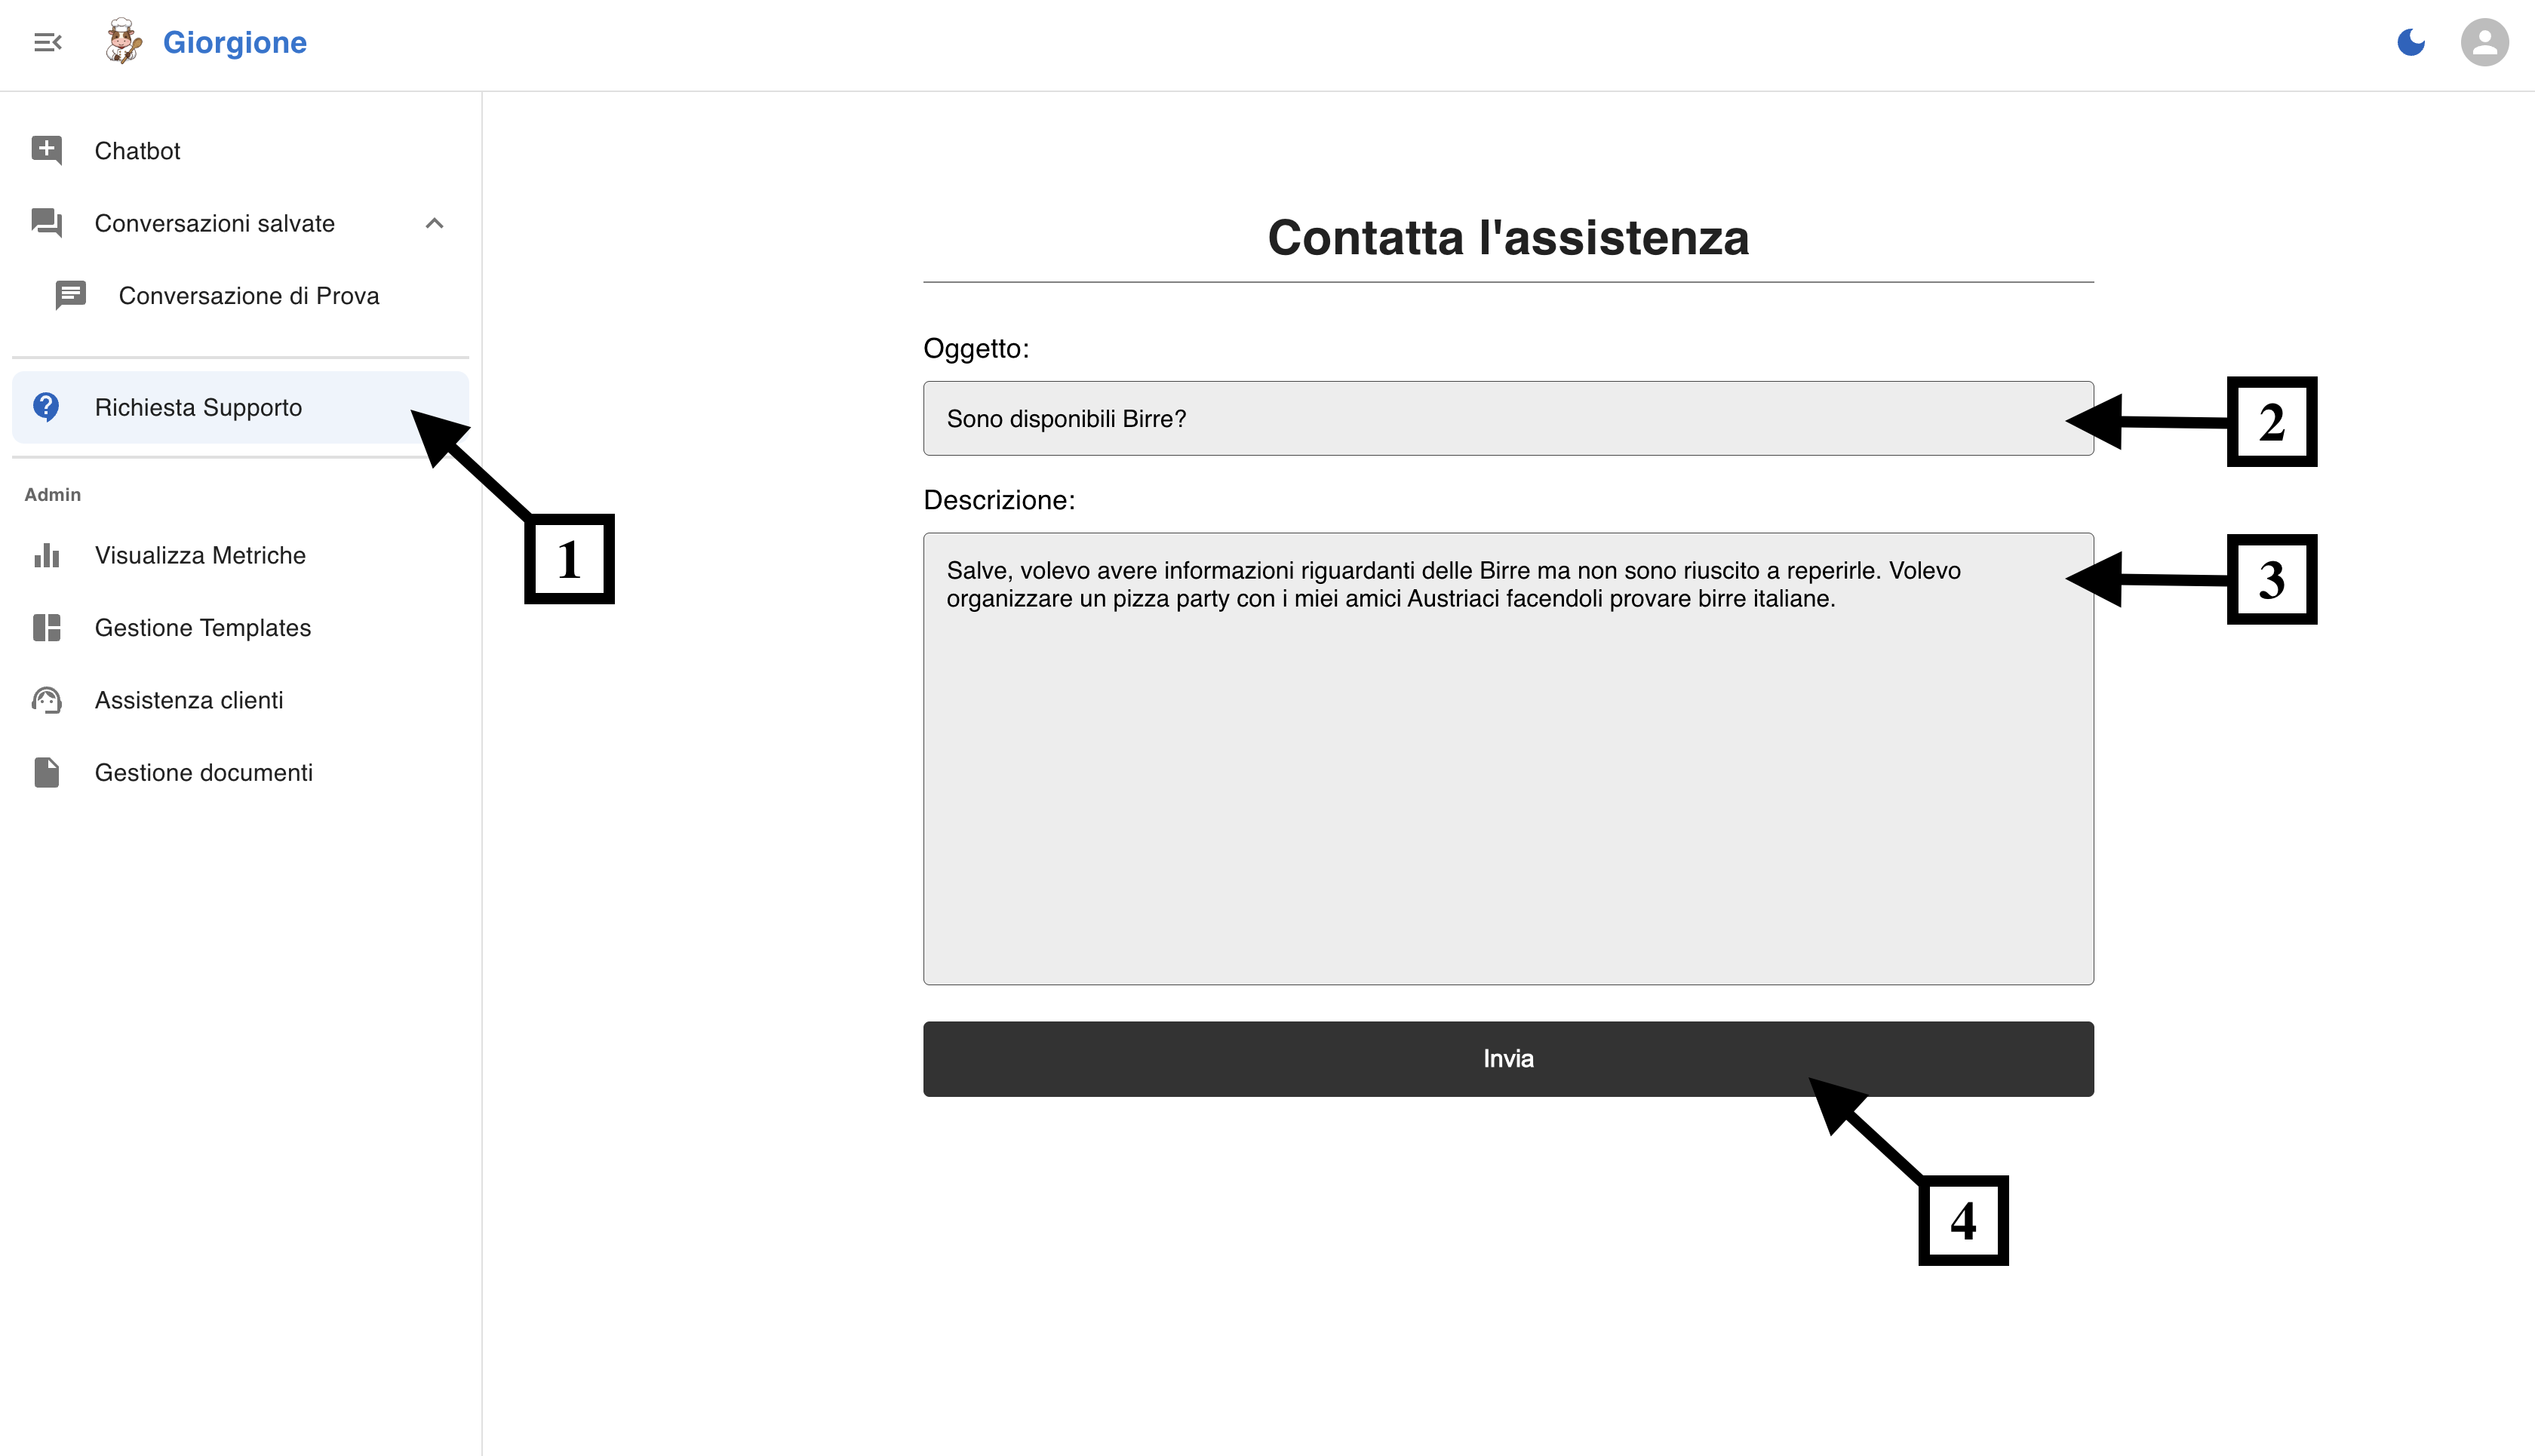
\includegraphics[width=\textwidth]{./img/RichiestaAssistenza1.png}
    \captionof{figure}{Pagina di Assistenza}
    \label{fig:Pagina di Assistenza}
\end{center}

\begin{center}
    
\includegraphics[width=0.8\textwidth]{./img/RichiestaAssistenza2.png}
    \captionof{figure}{Invio Richiesta Assistenza Riuscita}
    \label{fig:InvioRiuscito}
\end{center}

\subsubsection{Logout}
Cliccando sull’icona utente in alto a destra è possibile effettuare il logout e tornare alla pagina di login.
\begin{center}
    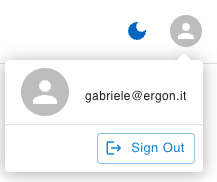
\includegraphics[width=0.3\textwidth]{./img/logout.png}
    \captionof{figure}{Logout}
\end{center}

\newpage
\subsection{Pagine riservate all'admin}

\subsubsection{Visualizza Metriche}
La dashboard delle metriche mostra like, dislike e numero totale di messaggi gestiti.
\begin{center}
    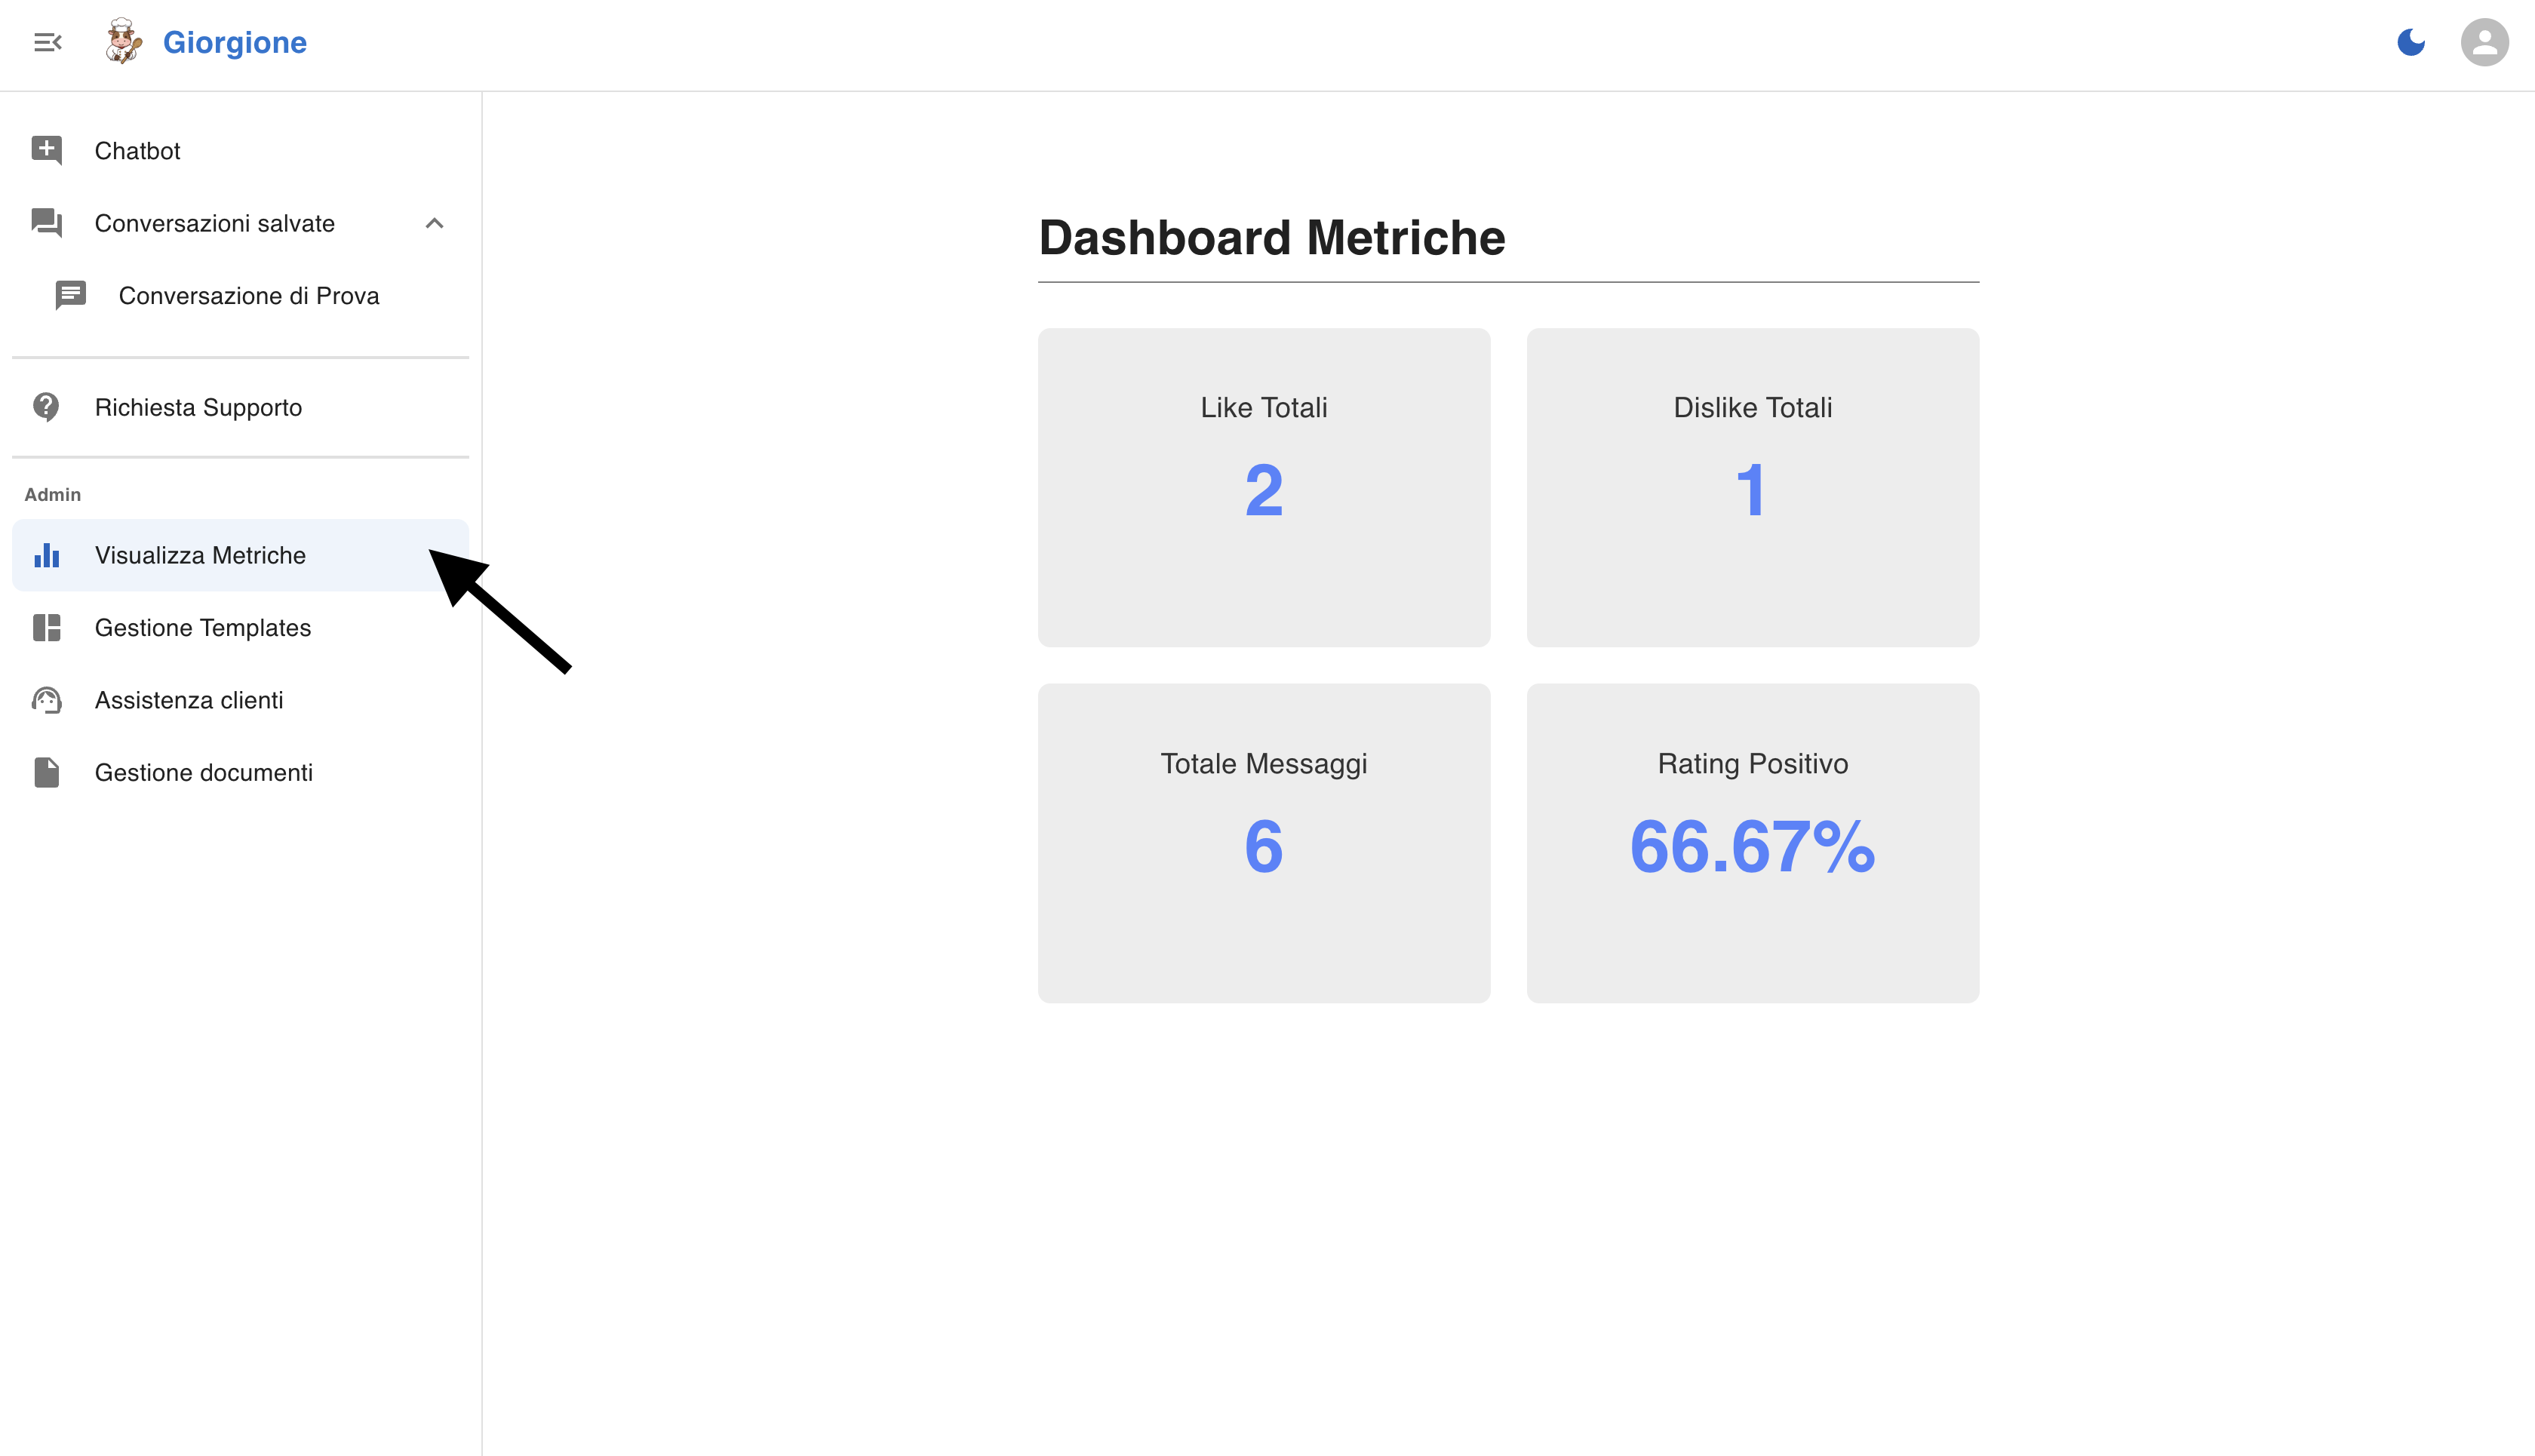
\includegraphics[width=\textwidth]{./img/visualizzaMetriche.png}
    \captionof{figure}{Dashboard Metriche}
    \label{fig:Metriche}
\end{center}

\subsubsection{Gestione Template}
Dalla voce "Gestione Template" si accede all’elenco dei template creati. È possibile aggiungerne, modificarli o eliminarli.
\begin{center}
    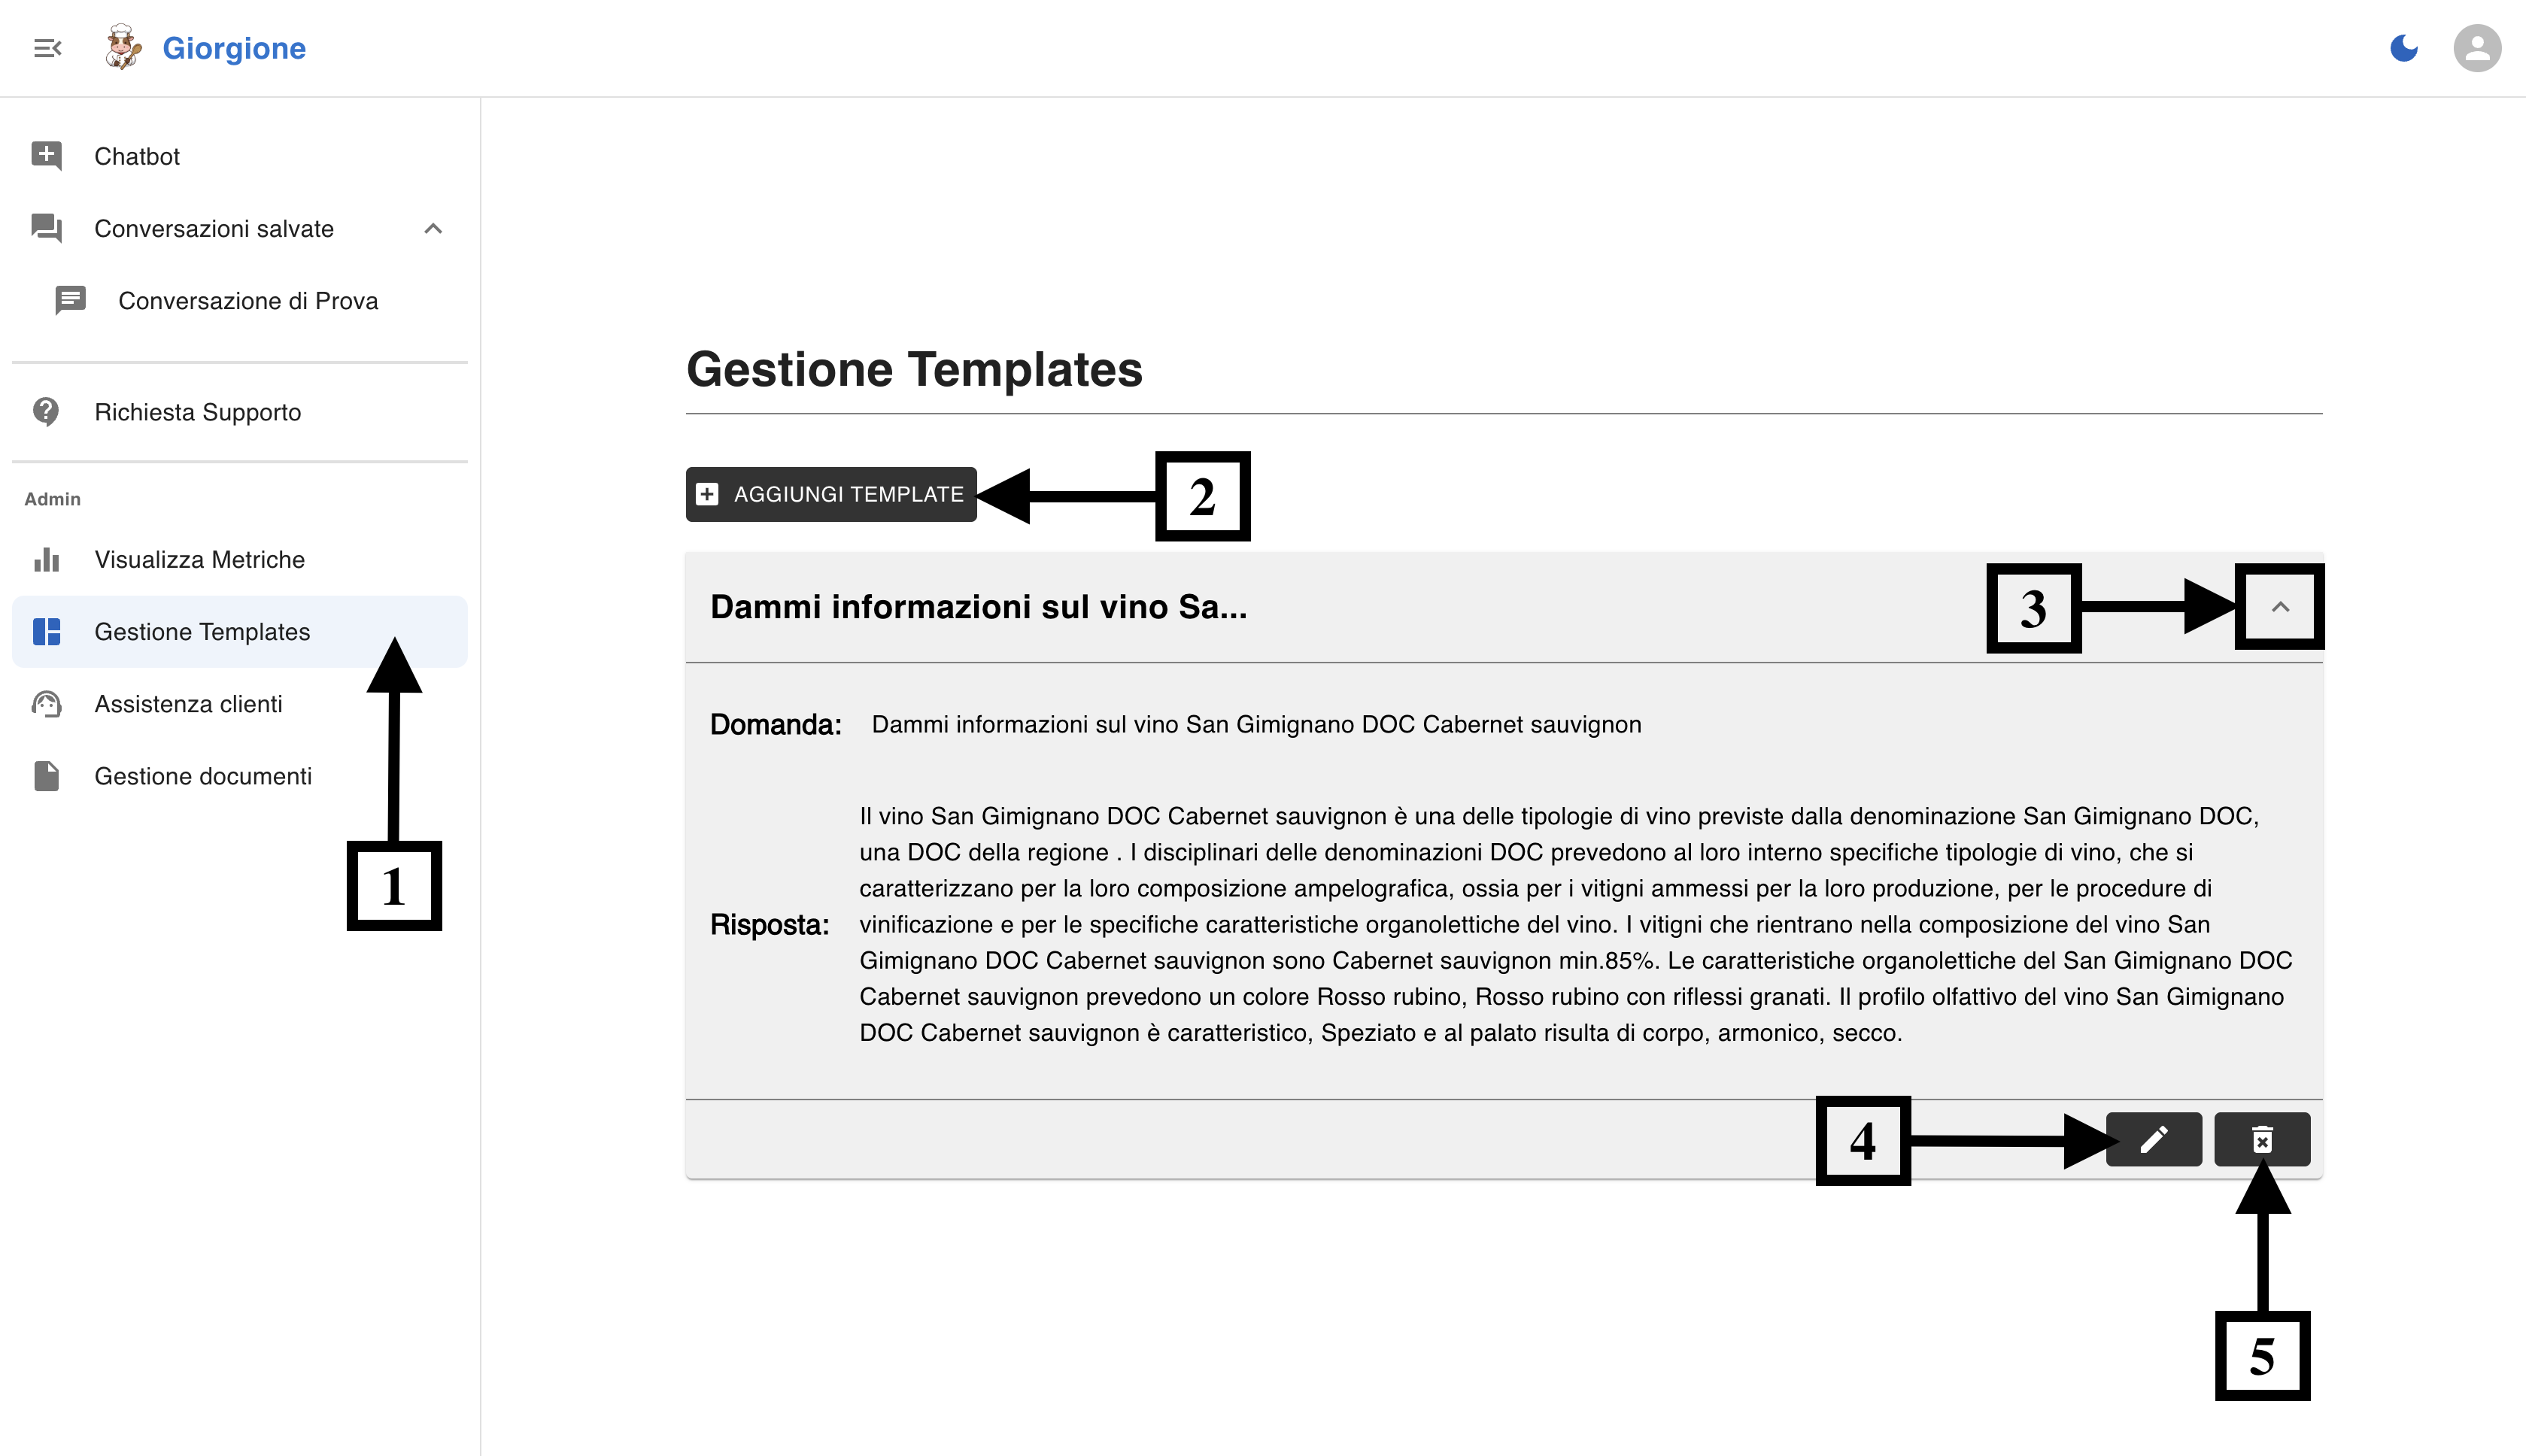
\includegraphics[width=\textwidth]{./img/GestioneTemplate.png}
    \captionof{figure}{Gestione Template}
    \label{fig:Template}
\end{center}

\begin{center}
    \includegraphics[width=0.4\textwidth]{./img/AggiungiTemplate.png}
    \captionof{figure}{Aggiunta nuovo template}
    \label{fig:addTemplate}
\end{center}

\begin{center}
    \includegraphics[width=0.5\textwidth]{./img/ModificaTemplate.png}
    \hspace{0.05\textwidth}
    \includegraphics[width=\textwidth]{./img/EliminaTemplate.png}
    \captionof{figure}{Modifica ed Eliminazione template}
    \label{fig:pop-up modifica ed elimina}
\end{center}

\subsubsection{Assistenza Clienti}
In questa sezione l’admin può visualizzare tutte le richieste degli utenti, verificarne lo stato e prenderle in carico.
\begin{center}
    \includegraphics[width=\textwidth]{./img/Assistenza1.png}
    \captionof{figure}{Gestione Assistenza}
    \label{fig:Assistenza1}
\end{center}

\begin{center}
    \includegraphics[width=0.5\textwidth]{./img/Assistenza2.png}
    \captionof{figure}{Cambio colore stato richiesta}
\end{center}

\subsubsection{Gestione Documenti}
L'admin può caricare documenti \texttt{.pdf} e \texttt{.txt} per addestrare l’assistente.
\begin{center}
    \includegraphics[width=0.8\textwidth]{./img/PaginaGestioneDocumenti1.png}
    \captionof{figure}{Pagina Gestione Documenti}
    \label{fig:gestione1}
\end{center}

\begin{center}
    \includegraphics[width=0.6\textwidth]{./img/PaginaGestioneDocumenti2.png}
    \captionof{figure}{Upload Documenti}
    \label{fig:gestione2}
\end{center}

\begin{center}
    \includegraphics[width=0.4\textwidth]{./img/PaginaGestioneDocumenti3.png}
    \hspace{0.05\textwidth}
    \includegraphics[width=0.4\textwidth]{./img/GestioneDocumenti4.png}
    \captionof{figure}{Inserimento file}
    \label{fig:gestione3}
\end{center}

\begin{center}
    \includegraphics[width=0.8\textwidth]{./img/GestioneDocumenti5.png}
    \captionof{figure}{Conferma upload documenti}
    \label{fig:gestione4}
\end{center}


\newpage

\section{Funzioni aggiuntive}

\newpage

\section{Supporto}

\end{document}
